% ============================================================
% Descrição das figuras geradas para o trabalho de mestrado
% Arquivo: descricao_figuras.tex
%
% Inclua este arquivo no preamble do Overleaf com:
%   % ============================================================
% Descrição das figuras geradas para o trabalho de mestrado
% Arquivo: descricao_figuras.tex
%
% Inclua este arquivo no preamble do Overleaf com:
%   % ============================================================
% Descrição das figuras geradas para o trabalho de mestrado
% Arquivo: descricao_figuras.tex
%
% Inclua este arquivo no preamble do Overleaf com:
%   % ============================================================
% Descrição das figuras geradas para o trabalho de mestrado
% Arquivo: descricao_figuras.tex
%
% Inclua este arquivo no preamble do Overleaf com:
%   \input{descricao_figuras}
% Ou copie as seções diretamente para o corpo do documento.
%
% As figuras devem estar na mesma pasta deste arquivo (.tex) no
% projeto Overleaf, com os nomes exatos referenciados abaixo.
% ============================================================

\documentclass[12pt]{article}
\usepackage[utf8]{inputenc}
\usepackage[T1]{fontenc}
\usepackage[portuguese]{babel}
\usepackage{graphicx}
\usepackage{float}
\usepackage{amsmath}
\usepackage{geometry}
\geometry{a4paper, margin=2.5cm}

\begin{document}

% ------------------------------------------------------------
\section*{Descrição das Figuras Geradas}

Este documento descreve as sete figuras geradas a partir dos resultados
experimentais da campanha de meta-heurísticas para otimização de alocação de
recursos em \textit{slices} de redes 5G/O-RAN. As figuras cobrem os três
cenários finalizados: \textbf{Low Traffic}, \textbf{Normal} e
\textbf{Congestion}. Os dados foram coletados a partir de 3 \textit{seeds}
aleatórias independentes (1, 2 e 3), com 300 avaliações da função objetivo por
par (cenário, \textit{seed}).

% ------------------------------------------------------------
\subsection*{Figura 1 -- Curvas de convergência das meta-heurísticas}

\begin{figure}[H]
    \centering
    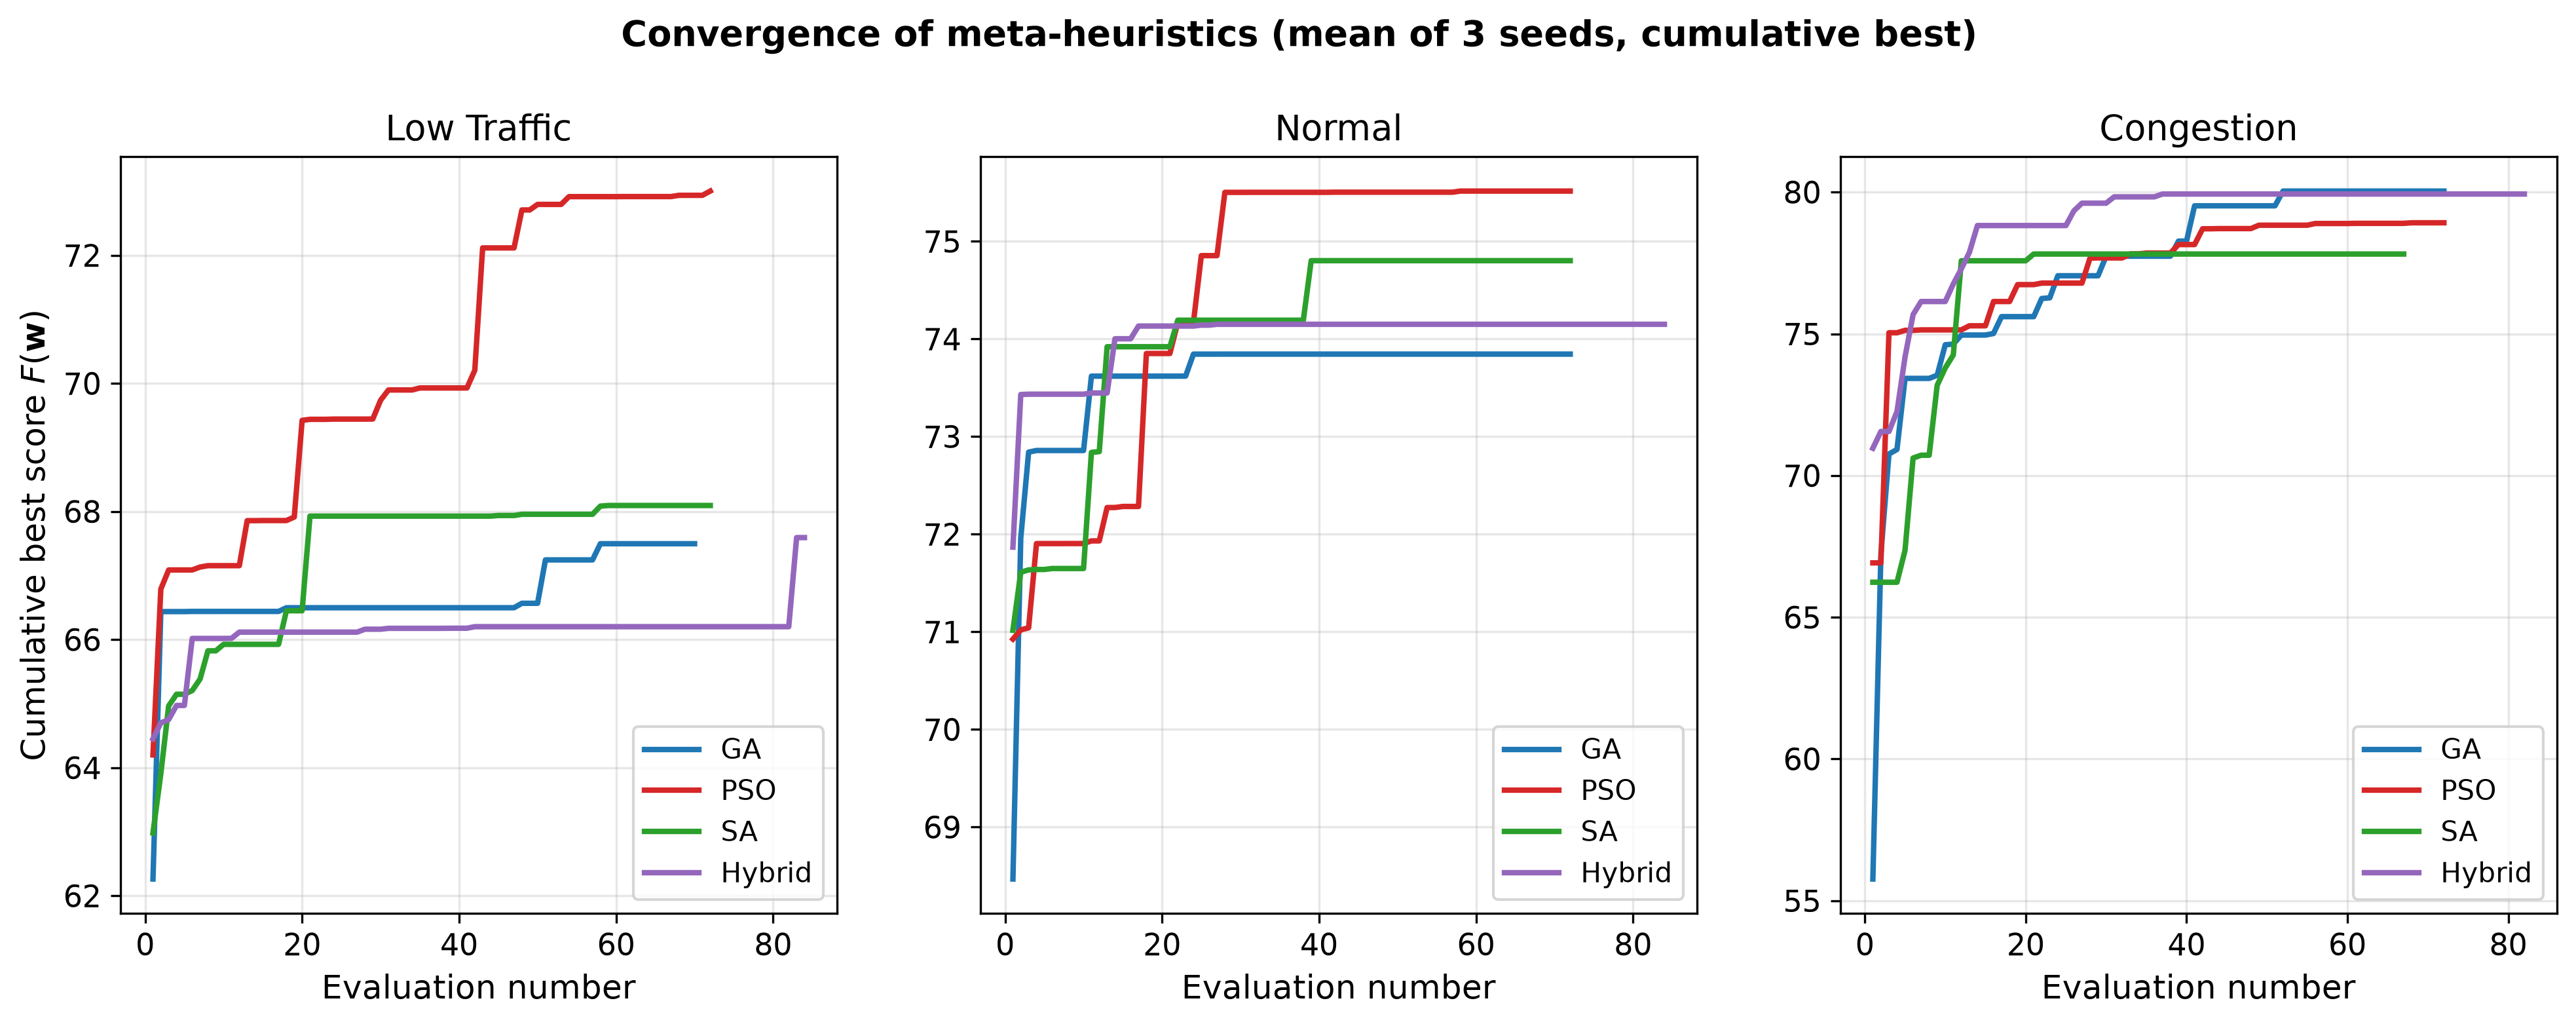
\includegraphics[width=\textwidth]{fig01_convergencia.png}
    \caption{Convergência das meta-heurísticas (média de 3 \textit{seeds}, melhor-acumulado).}
    \label{fig:convergencia}
\end{figure}

A Figura~\ref{fig:convergencia} apresenta as curvas de convergência dos quatro
algoritmos avaliados (GA, PSO, SA e Híbrida), expressando o melhor
\textit{score} acumulado $F(\mathbf{w})$ em função do número de avaliações da
função objetivo. Cada subplot corresponde a um cenário de tráfego. A curva
monotônica (melhor-acumulado) permite comparar a velocidade de convergência e
o valor final alcançado por cada meta-heurística, evidenciando qual método
identifica regiões promissoras do espaço de busca mais rapidamente.

% ------------------------------------------------------------
\subsection*{Figura 2 -- Distribuição dos \textit{scores} por meta-heurística}

\begin{figure}[H]
    \centering
    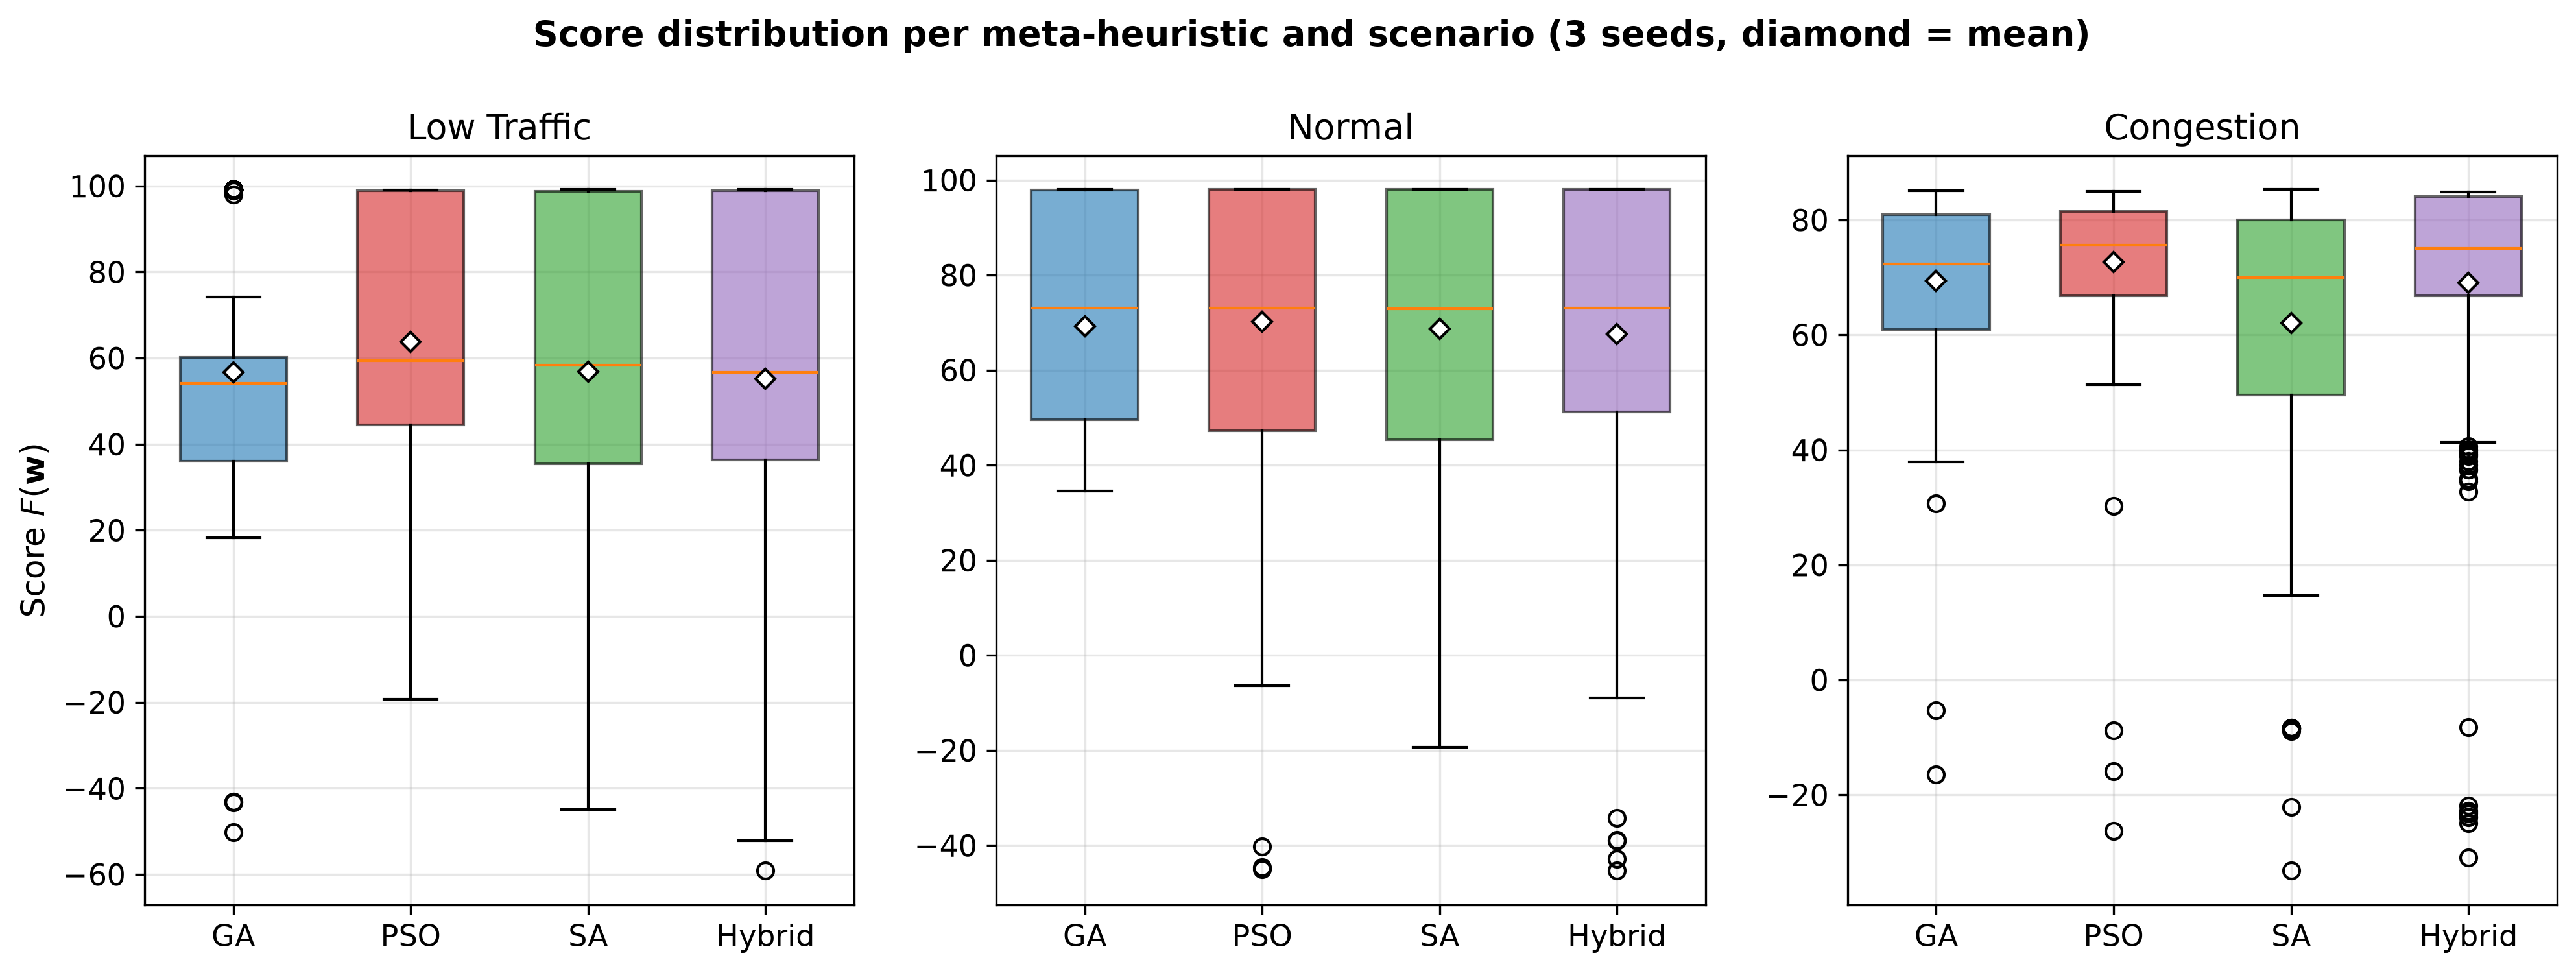
\includegraphics[width=\textwidth]{fig02_distribuicao_scores.png}
    \caption{Distribuição dos \textit{scores} por meta-heurística e cenário (3 \textit{seeds}, $\diamond$ = média).}
    \label{fig:distribuicao}
\end{figure}

A Figura~\ref{fig:distribuicao} mostra a distribuição estatística dos
\textit{scores} obtidos por cada meta-heurística durante a busca, na forma de
\textit{boxplots}. Cada \textit{boxplot} resume as ~72--84 avaliações de cada
método, agregando as 3 \textit{seeds}. O losango ($\diamond$) indica a média.
Esta figura é importante para avaliar não apenas o melhor resultado
(\textit{score} máximo), mas também a variabilidade e a estabilidade de cada
algoritmo: métodos com \textit{boxes} mais estreitos e medianas altas são
preferíveis sob a ótica de robustez, mesmo que o valor máximo seja similar ao
de um concorrente mais instável.

% ------------------------------------------------------------
\subsection*{Figura 3 -- Comparação entre meta-heurísticas e \textit{baselines}}

\begin{figure}[H]
    \centering
    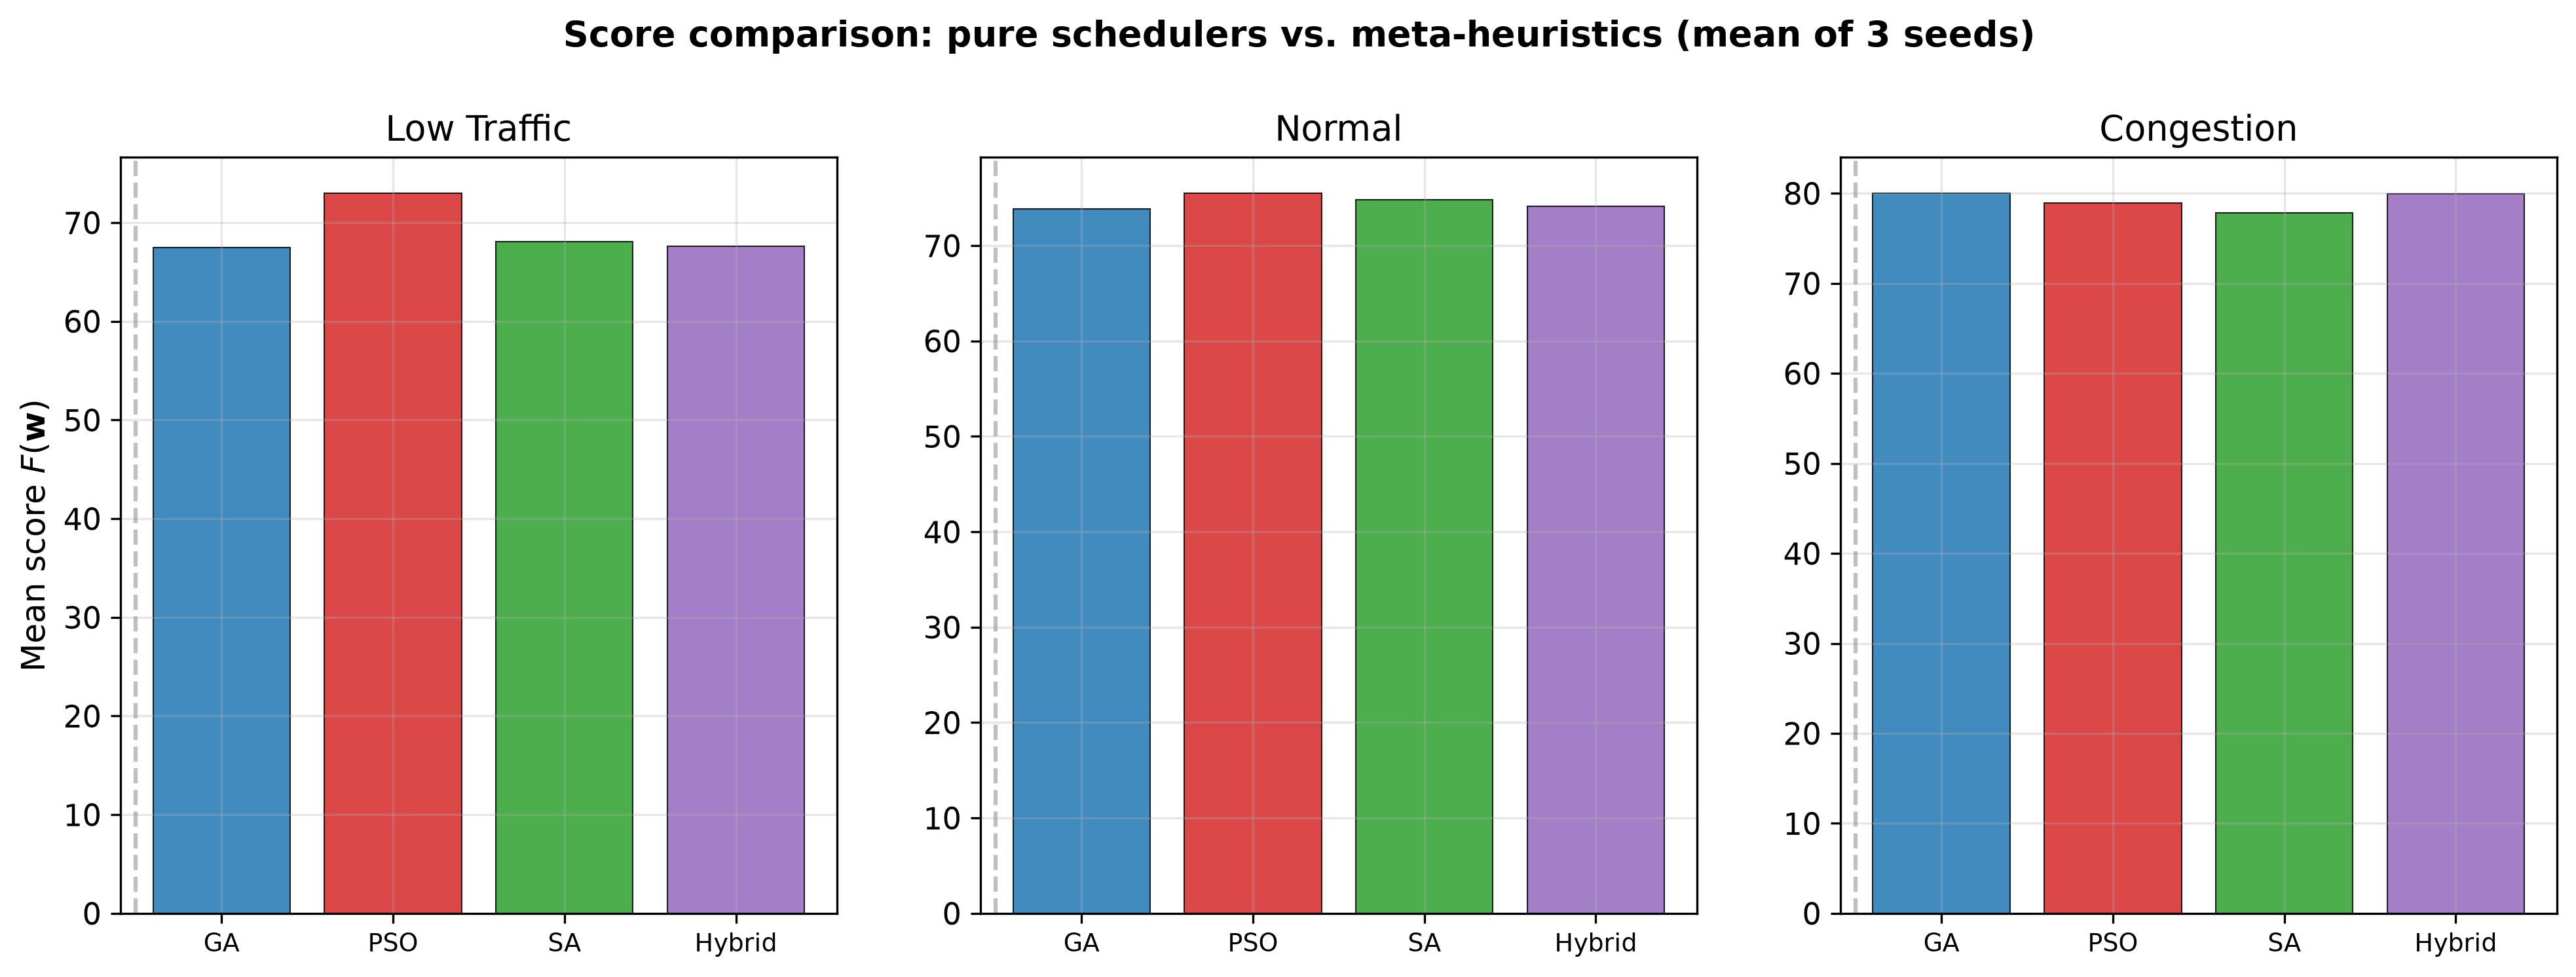
\includegraphics[width=\textwidth]{fig03_comparacao_baselines.png}
    \caption{Comparação do \textit{score} médio entre \textit{schedulers} puros, heurísticas adaptativas e meta-heurísticas.}
    \label{fig:comparacao}
\end{figure}

A Figura~\ref{fig:comparacao} confronta o desempenho das meta-heurísticas (GA,
PSO, SA e Híbrida) com os \textit{baselines} de referência: os
\textit{schedulers} puros clássicos (RR, PF, BCQI) e as heurísticas
adaptativas (Weighted PF, AQPS, Meta-Risk Elastic). As barras representam o
\textit{score} médio $F(\mathbf{w})$ das 3 \textit{seeds}. A linha tracejada
separa os métodos adaptativos/determinísticos (à esquerda) das
meta-heurísticas propostas (à direita). Esta comparação direto responde à
pergunta central da pesquisa: a otimização dos pesos de alocação
offline traz ganho mensurável em relação às abordagens clássicas?

% ------------------------------------------------------------
\subsection*{Figura 4 -- \textit{Trade-off} entre \textit{throughput} e justiça}

\begin{figure}[H]
    \centering
    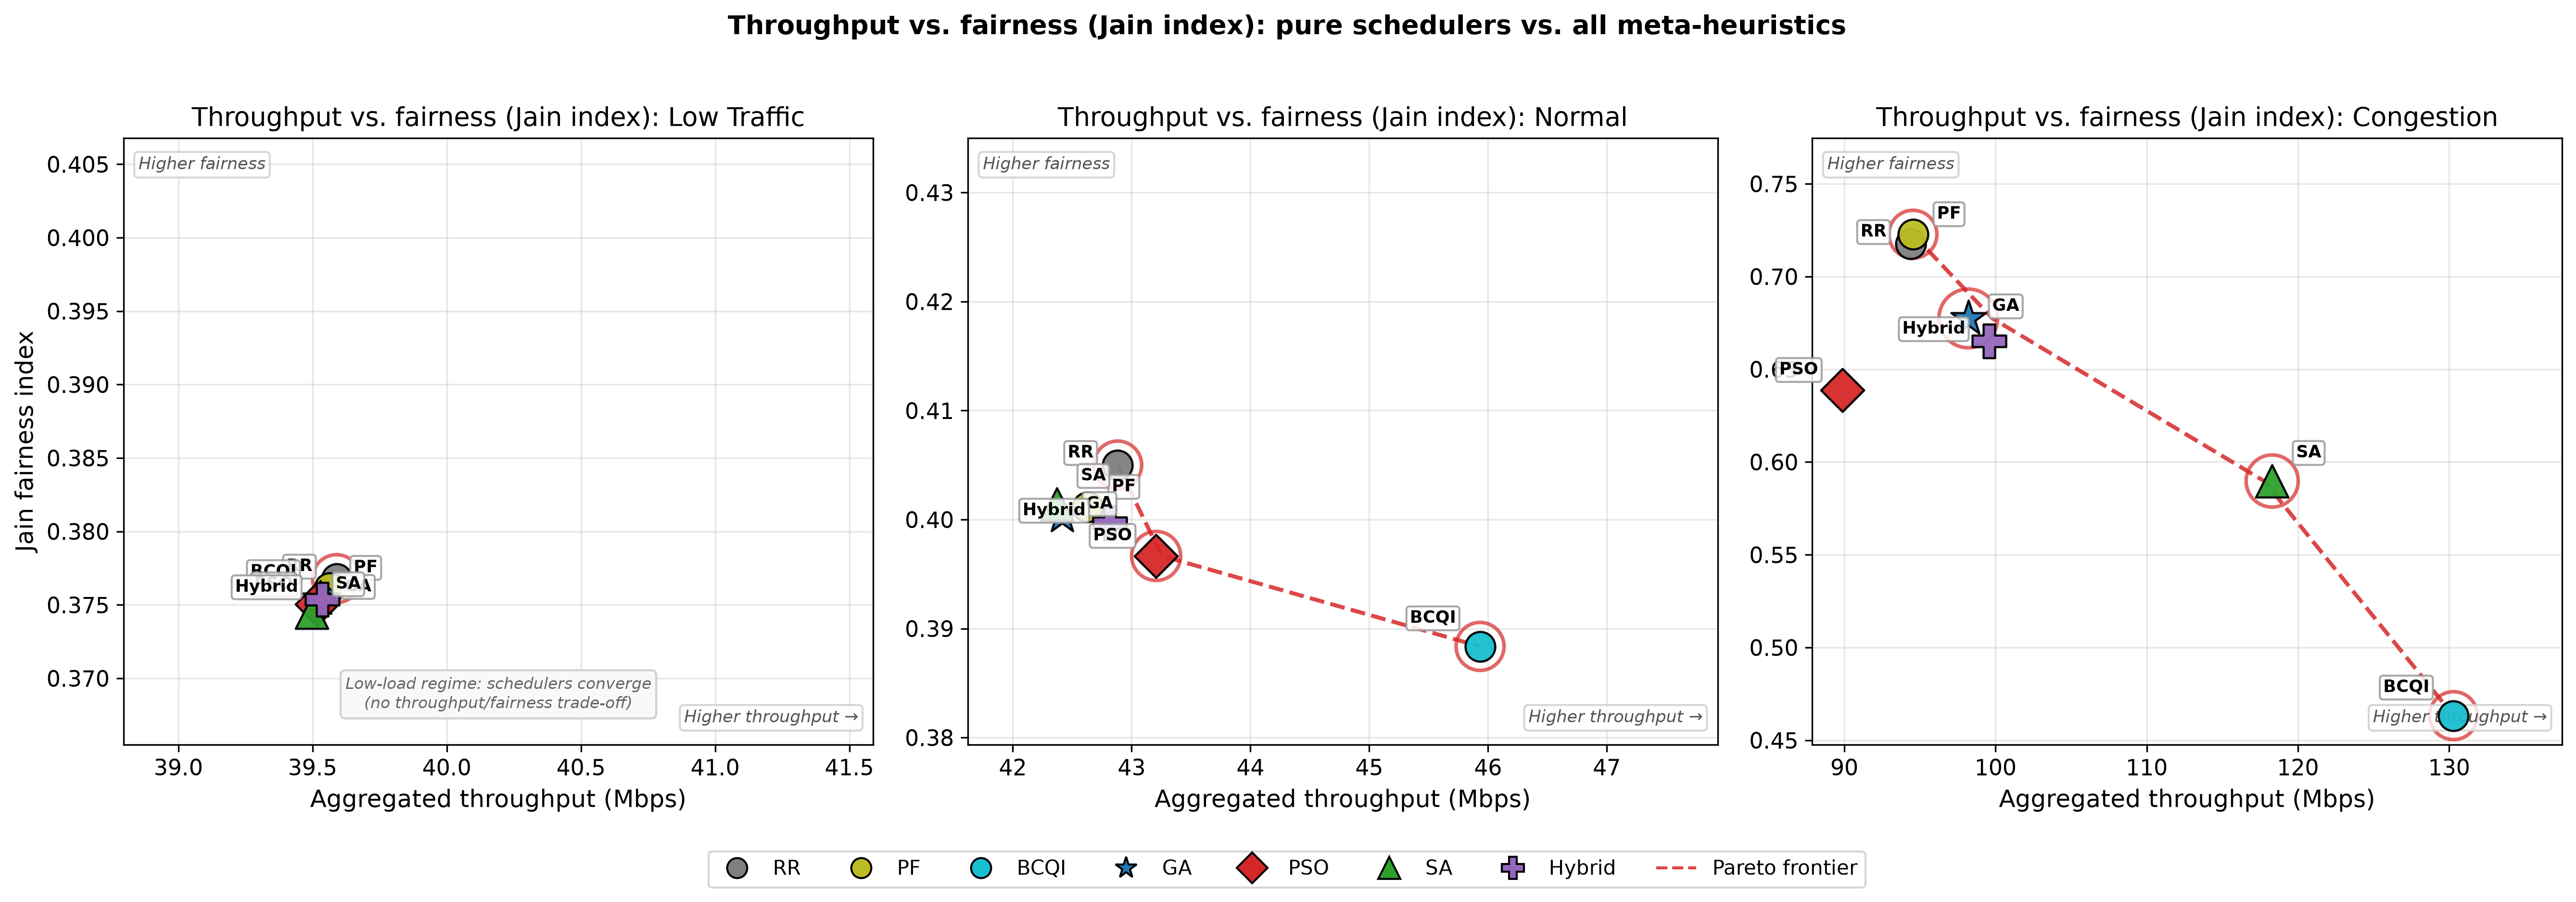
\includegraphics[width=0.85\textwidth]{fig04_tradeoff_pareto.png}
    \caption{\textit{Trade-off} entre \textit{throughput} agregado e a métrica de justiça/SLA (score $F$).}
    \label{fig:pareto}
\end{figure}

A Figura~\ref{fig:pareto} é a análise mais crítica do estudo: ela mapeia a
fronteira de Pareto entre o \textit{throughput} agregado da rede (eixo $x$) e a
função objetivo $F(\mathbf{w})$, que pondera satisfação de SLA, justiça e
latência (eixo $y$). Cada ponto representa um \textit{baseline} (média de 3
\textit{seeds}) em um cenário. Observa-se que os \textit{schedulers} puros,
em especial o BCQI, atingem alto \textit{throughput} agregado mas com baixo
\textit{score} de justiça (porque \textit{starvation} de \textit{slices}
frágeis como o MTC). As abordagens \textit{slice-aware}, ao particionar o
espectro por peso, sacrificam parte do \textit{throughput} total para
garantir que cada \textit{slice} receba uma cota proporcional, alcançando
maior $F(\mathbf{w})$. Esta figura fundamenta o argumento central do
trabalho: o \textit{network slicing} prioriza justiça e atendimento de SLA
sobre a maximização do \textit{throughput} bruto.

% ------------------------------------------------------------
\subsection*{Figura 5 -- Variabilidade entre \textit{seeds}}

\begin{figure}[H]
    \centering
    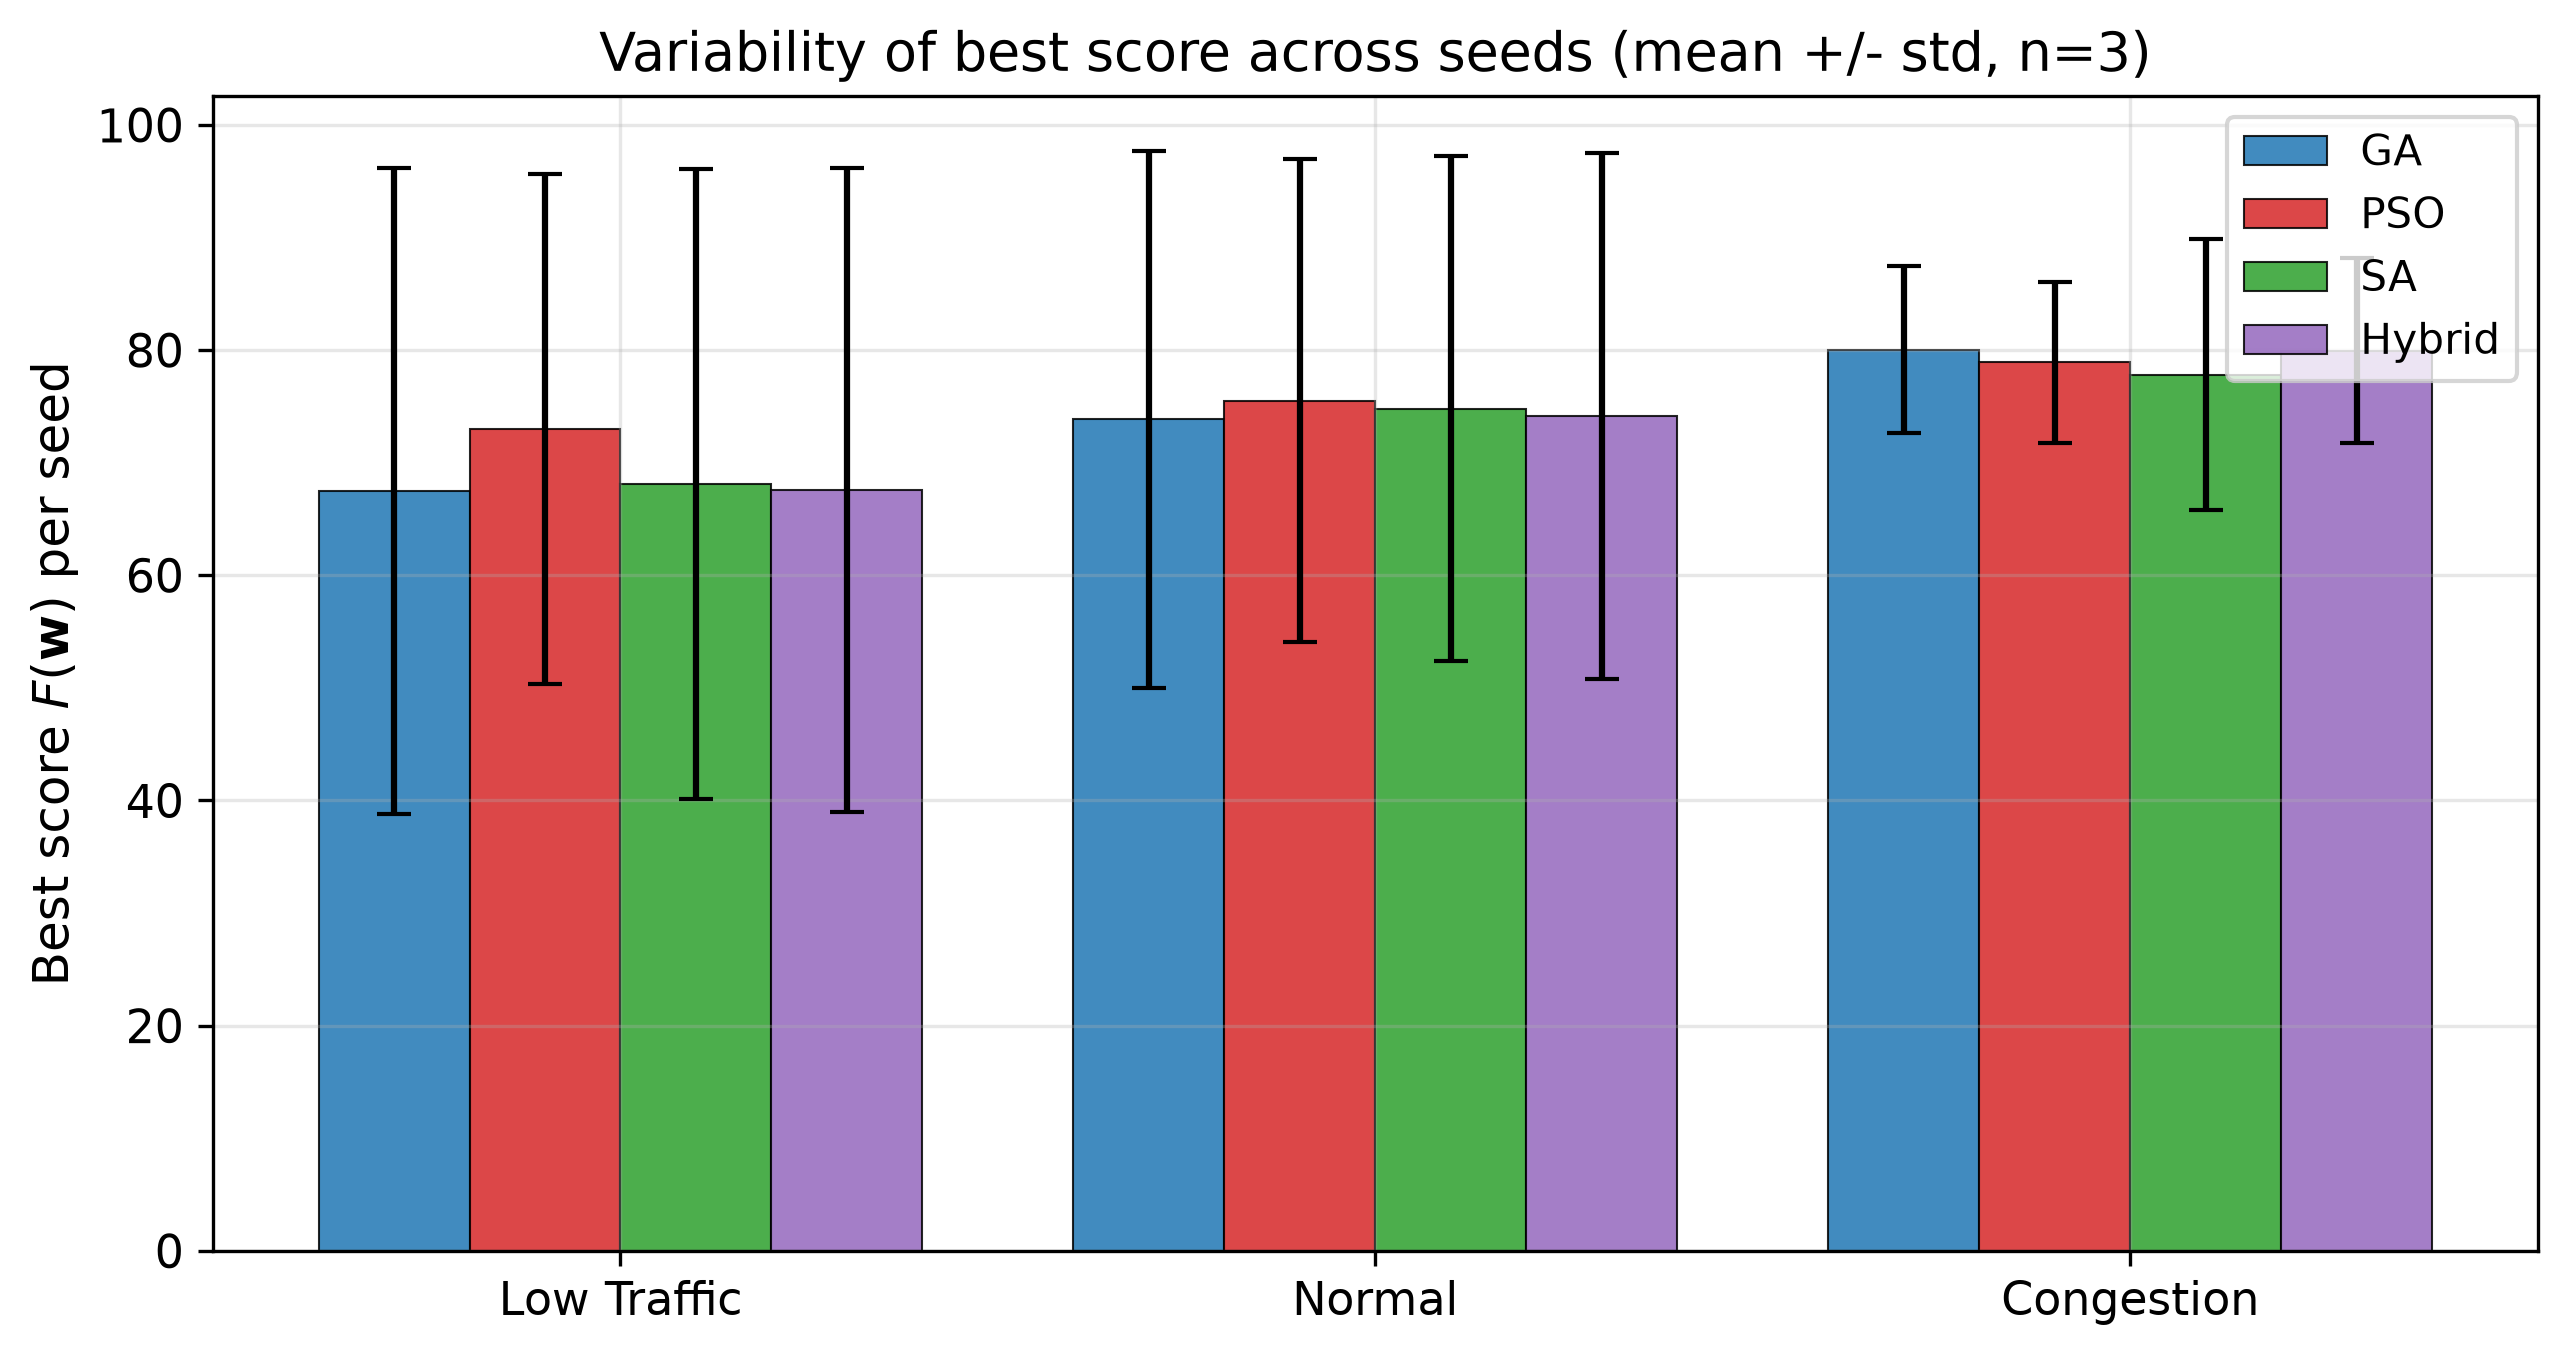
\includegraphics[width=0.9\textwidth]{fig05_variabilidade_seeds.png}
    \caption{Variabilidade do melhor \textit{score} entre \textit{seeds} (média $\pm$ desvio, $n=3$).}
    \label{fig:variabilidade}
\end{figure}

A Figura~\ref{fig:variabilidade} apresenta o melhor \textit{score} de cada
meta-heurística por cenário, com barras de erro representando o desvio-padrão
entre as 3 \textit{seeds} independentes. Esta visualização é fundamental para
a transparência metodológica: ela mostra que, com $n=3$, a variabilidade
entre execuções independentes (de 5 a 15 pontos de \textit{score}) pode ser da
mesma ordem de grandeza que a diferença entre os métodos, impossibilitando,
no momento, a declaração de significância estatística formal (que exigiria
$n \geq 5$ para testes como Wilcoxon ou Friedman). Este resultado negativo
honesto reforça a integridade da análise.

% ------------------------------------------------------------
\subsection*{Figura 6 -- Pesos ótimos encontrados}

\begin{figure}[H]
    \centering
    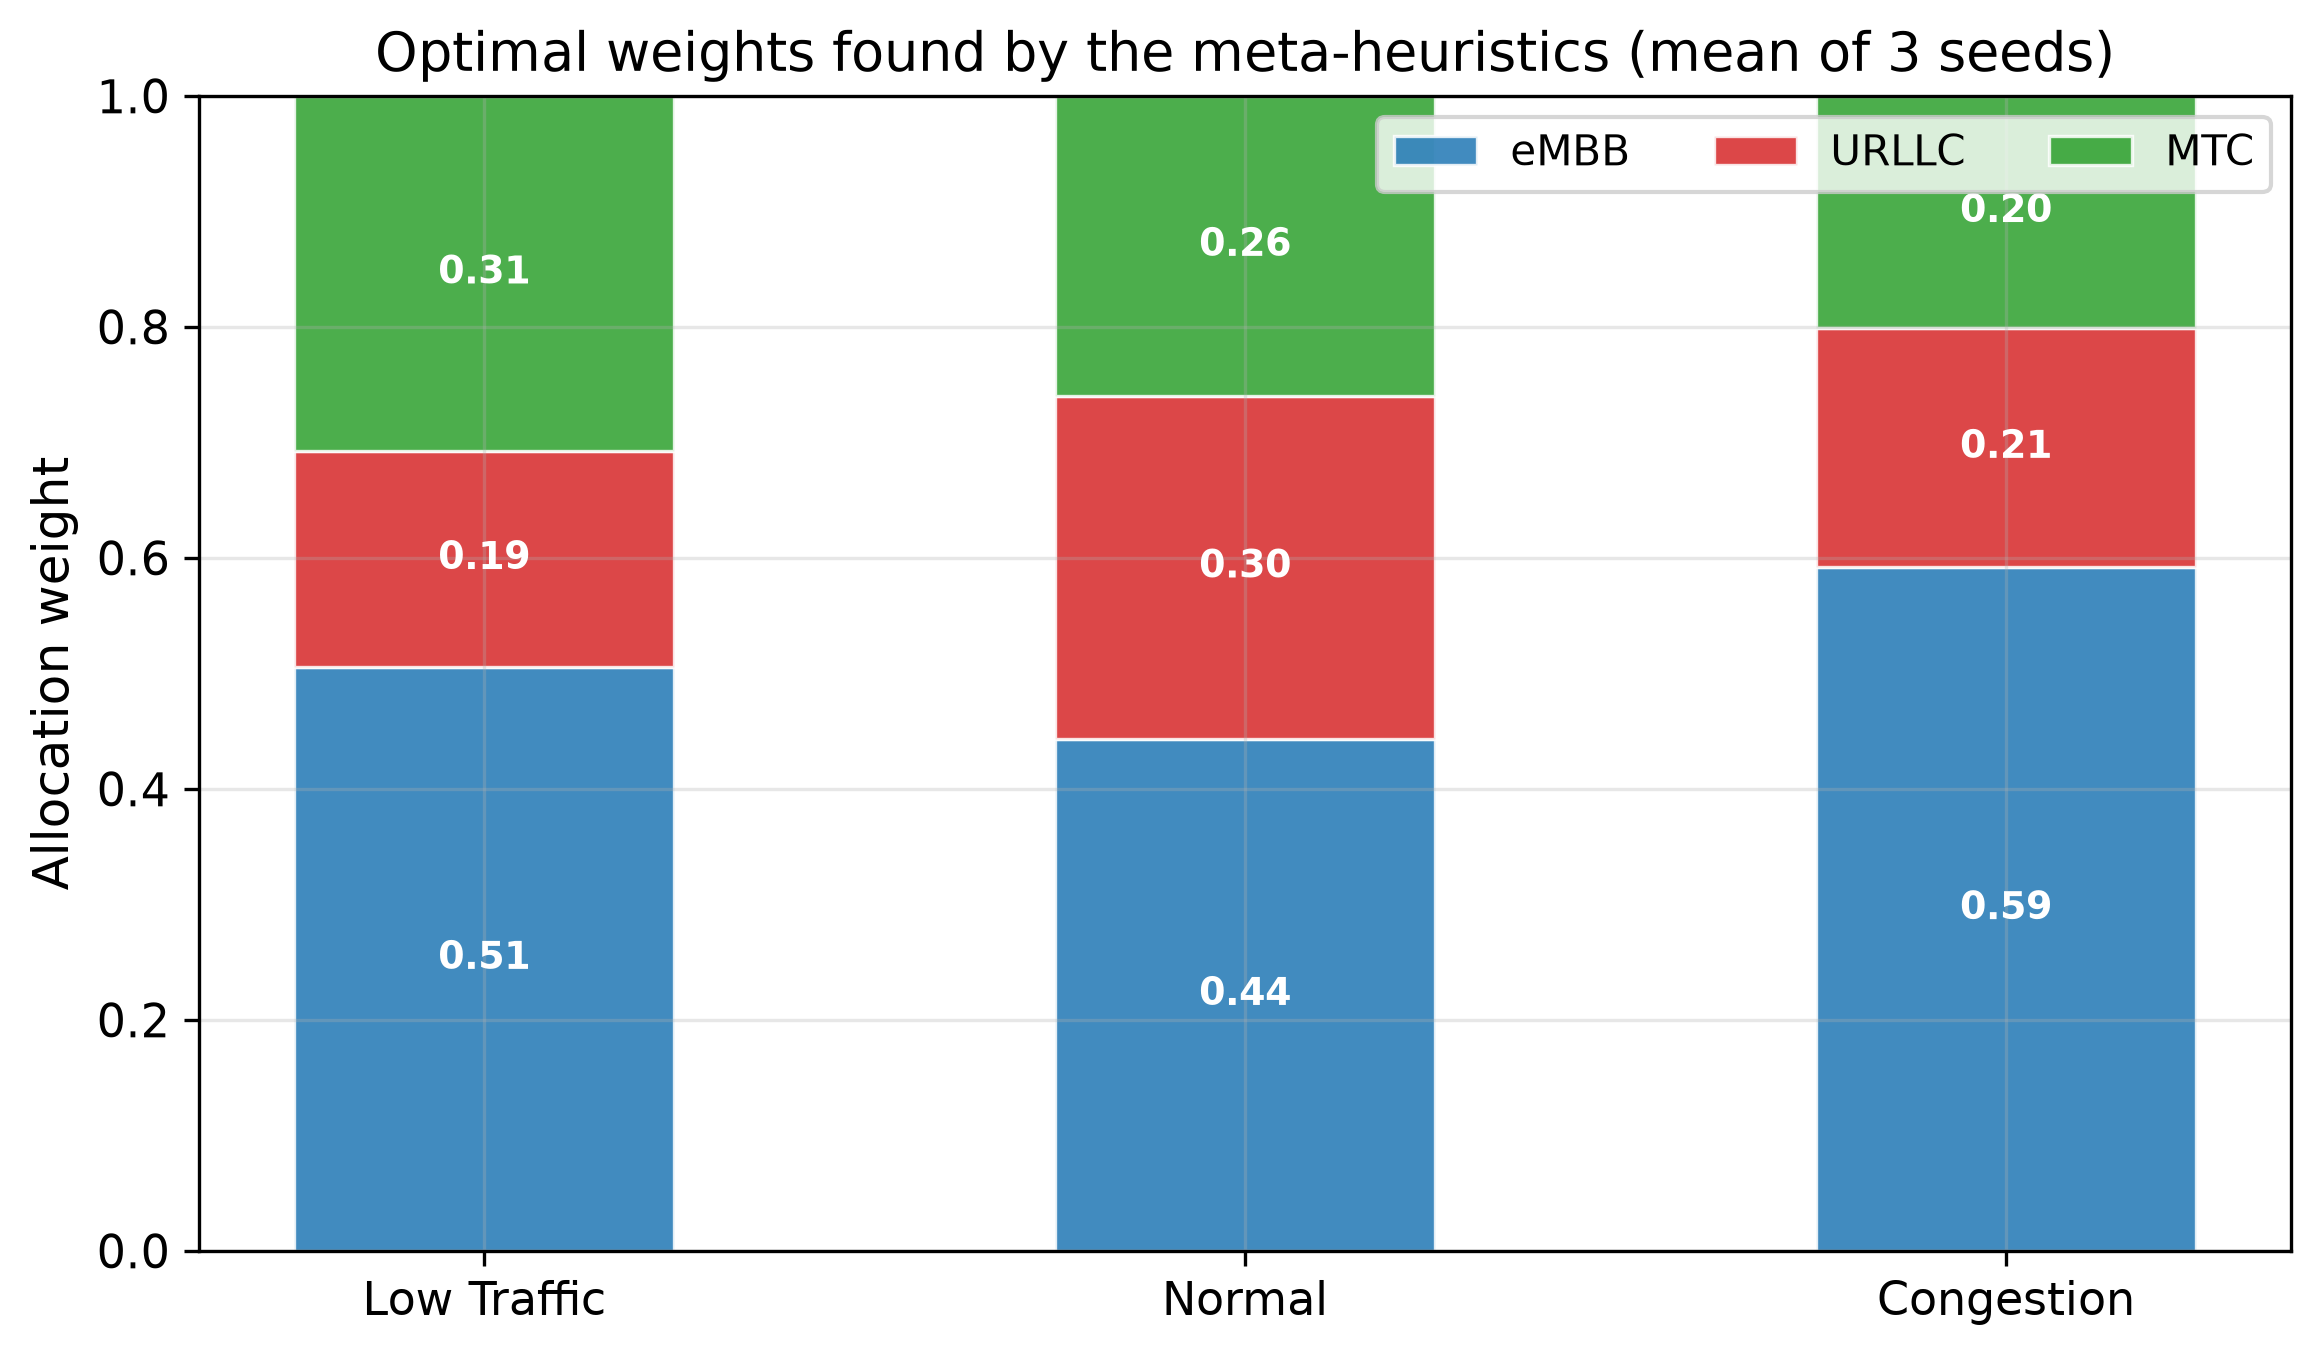
\includegraphics[width=0.8\textwidth]{fig06_pesos_otimos.png}
    \caption{Pesos ótimos $\mathbf{w}^* = [w_{eMBB}, w_{URLLC}, w_{MTC}]$ por cenário (média de 3 \textit{seeds}).}
    \label{fig:pesos}
\end{figure}

A Figura~\ref{fig:pesos} exibe os vetores de pesos ótimos
$\mathbf{w}^* = [w_{eMBB}, w_{URLLC}, w_{MTC}]$ identificados pela melhor
meta-heurística em cada cenário, agregados como a média das 3 \textit{seeds}.
As barras empilhadas (somando 1,0) revelam como o otimizador particiona o
orçamento de RBGs entre os três \textit{slices}. Espera-se que cenários mais
congestionados destinem maior peso ao \textit{slice} URLLC (sensível à
latência), dado que a função objetivo aplica uma forte penalidade por
violação do limite de 10\,ms. A análise destes pesos valida se o
comportamento do otimizador faz sentido físico do domínio 5G.

% ------------------------------------------------------------
\subsection*{Figura 7 -- \textit{Throughput} por \textit{slice}}

\begin{figure}[H]
    \centering
    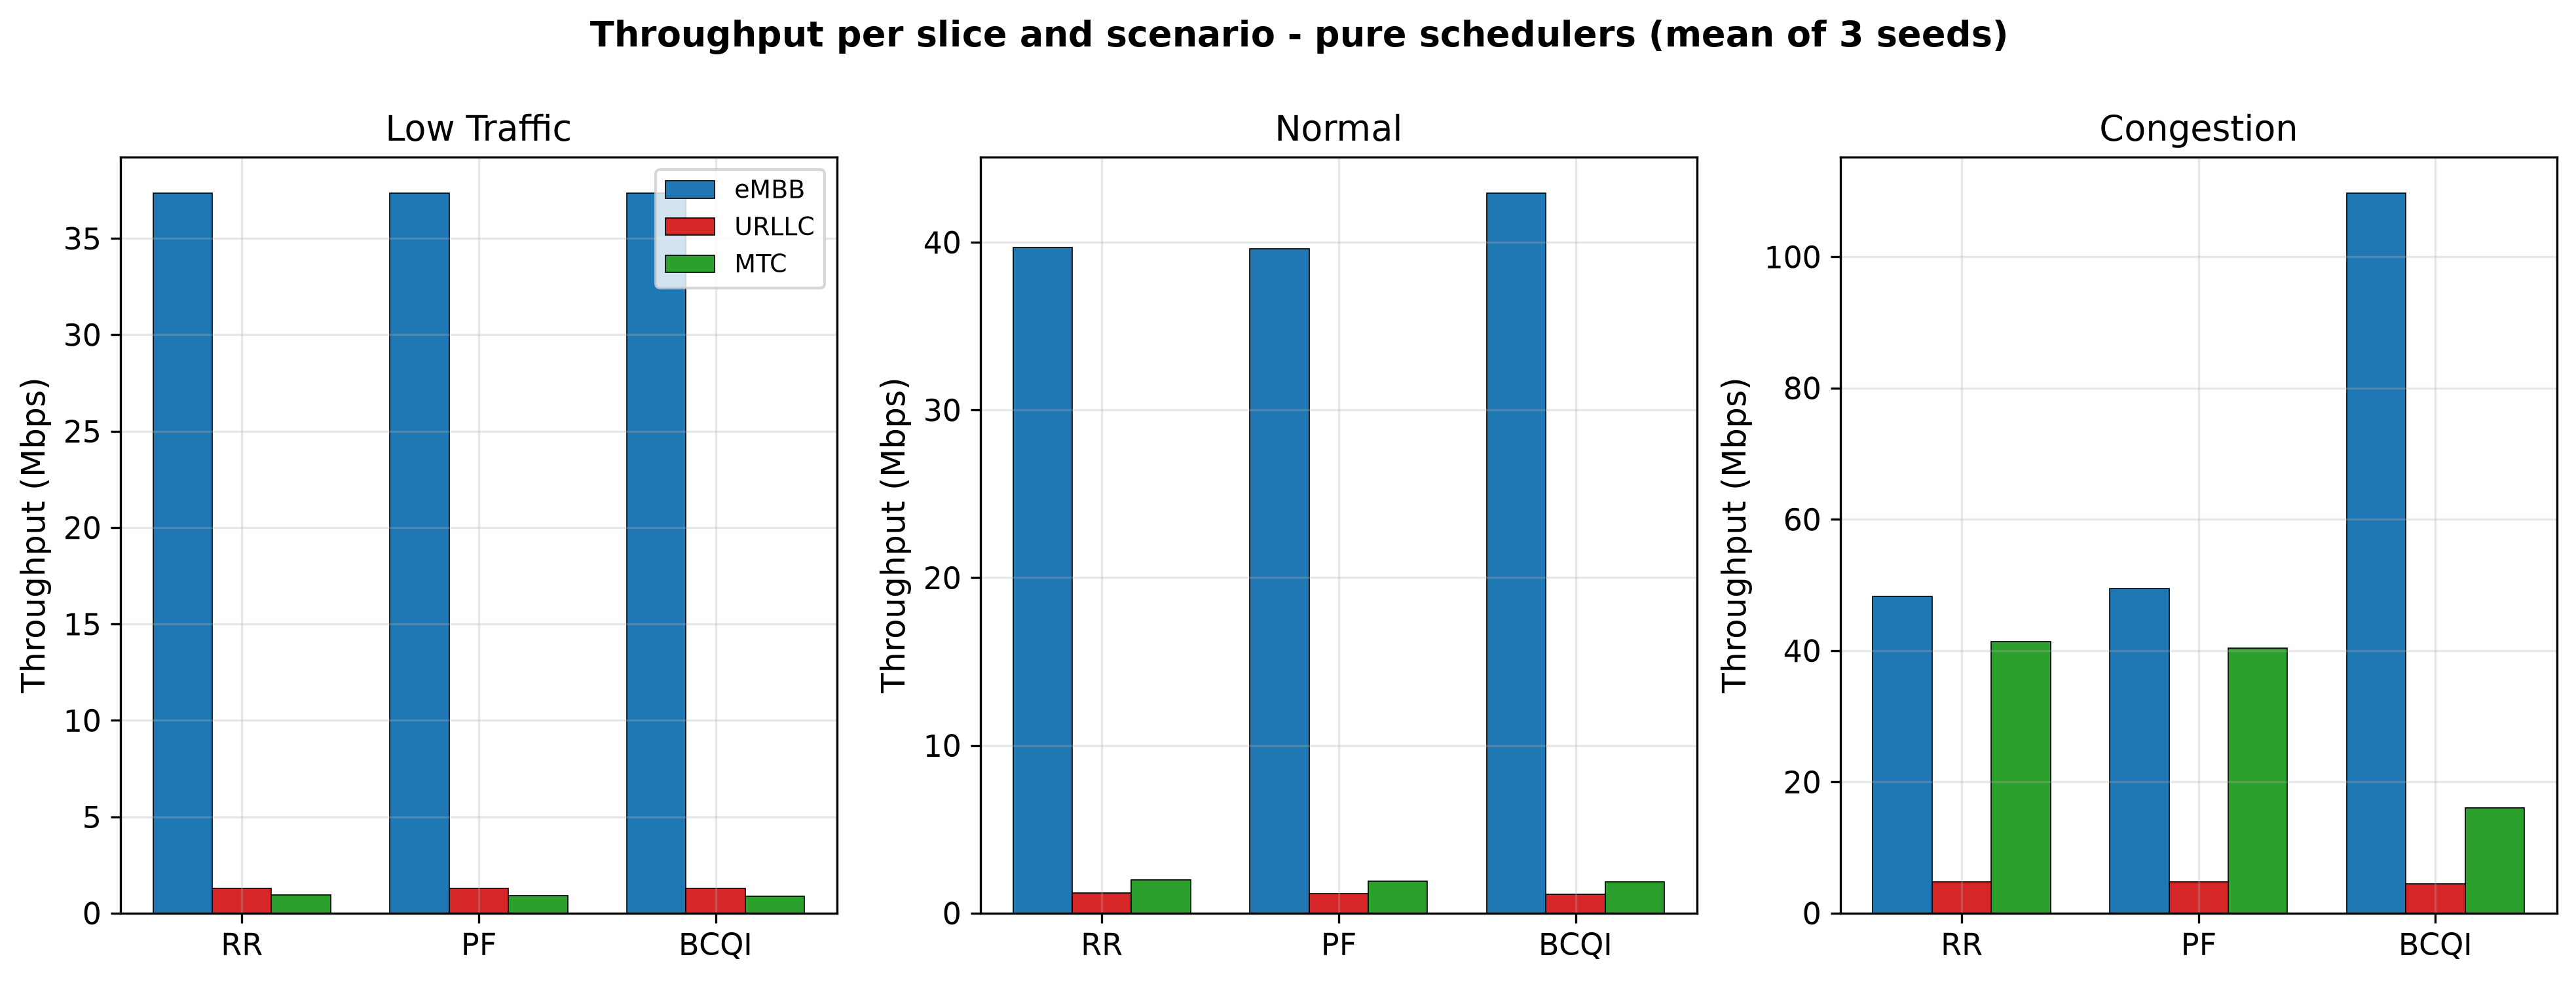
\includegraphics[width=\textwidth]{fig07_throughput_por_slice.png}
    \caption{\textit{Throughput} por \textit{slice} (eMBB, URLLC, MTC) e por cenário.}
    \label{fig:throughput_slice}
\end{figure}

A Figura~\ref{fig:throughput_slice} detalha o \textit{throughput} médio de cada
\textit{slice} individualmente (eMBB, URLLC e MTC) sob os diferentes
\textit{baselines}. Esta granularidade é essencial para entender o impacto
real das estratégias de alocação: enquanto um \textit{scheduler} puro pode
apresentar alto \textit{throughput} agregado (drenando recursos para um
\textit{slice} dominante, tipicamente o eMBB), as abordagens
\textit{slice-aware} distribuem o espectro de forma a manter todos os
\textit{slices} com vazão mínima compatível com seus SLAs. Em especial, o
comportamento do \textit{slice} MTC (composta de sensores IoT) sob alta
congestionamento evidencia os riscos de \textit{starvation} quando não há
isolamento entre \textit{slices}.

% ============================================================
\end{document}

% Ou copie as seções diretamente para o corpo do documento.
%
% As figuras devem estar na mesma pasta deste arquivo (.tex) no
% projeto Overleaf, com os nomes exatos referenciados abaixo.
% ============================================================

\documentclass[12pt]{article}
\usepackage[utf8]{inputenc}
\usepackage[T1]{fontenc}
\usepackage[portuguese]{babel}
\usepackage{graphicx}
\usepackage{float}
\usepackage{amsmath}
\usepackage{geometry}
\geometry{a4paper, margin=2.5cm}

\begin{document}

% ------------------------------------------------------------
\section*{Descrição das Figuras Geradas}

Este documento descreve as sete figuras geradas a partir dos resultados
experimentais da campanha de meta-heurísticas para otimização de alocação de
recursos em \textit{slices} de redes 5G/O-RAN. As figuras cobrem os três
cenários finalizados: \textbf{Low Traffic}, \textbf{Normal} e
\textbf{Congestion}. Os dados foram coletados a partir de 3 \textit{seeds}
aleatórias independentes (1, 2 e 3), com 300 avaliações da função objetivo por
par (cenário, \textit{seed}).

% ------------------------------------------------------------
\subsection*{Figura 1 -- Curvas de convergência das meta-heurísticas}

\begin{figure}[H]
    \centering
    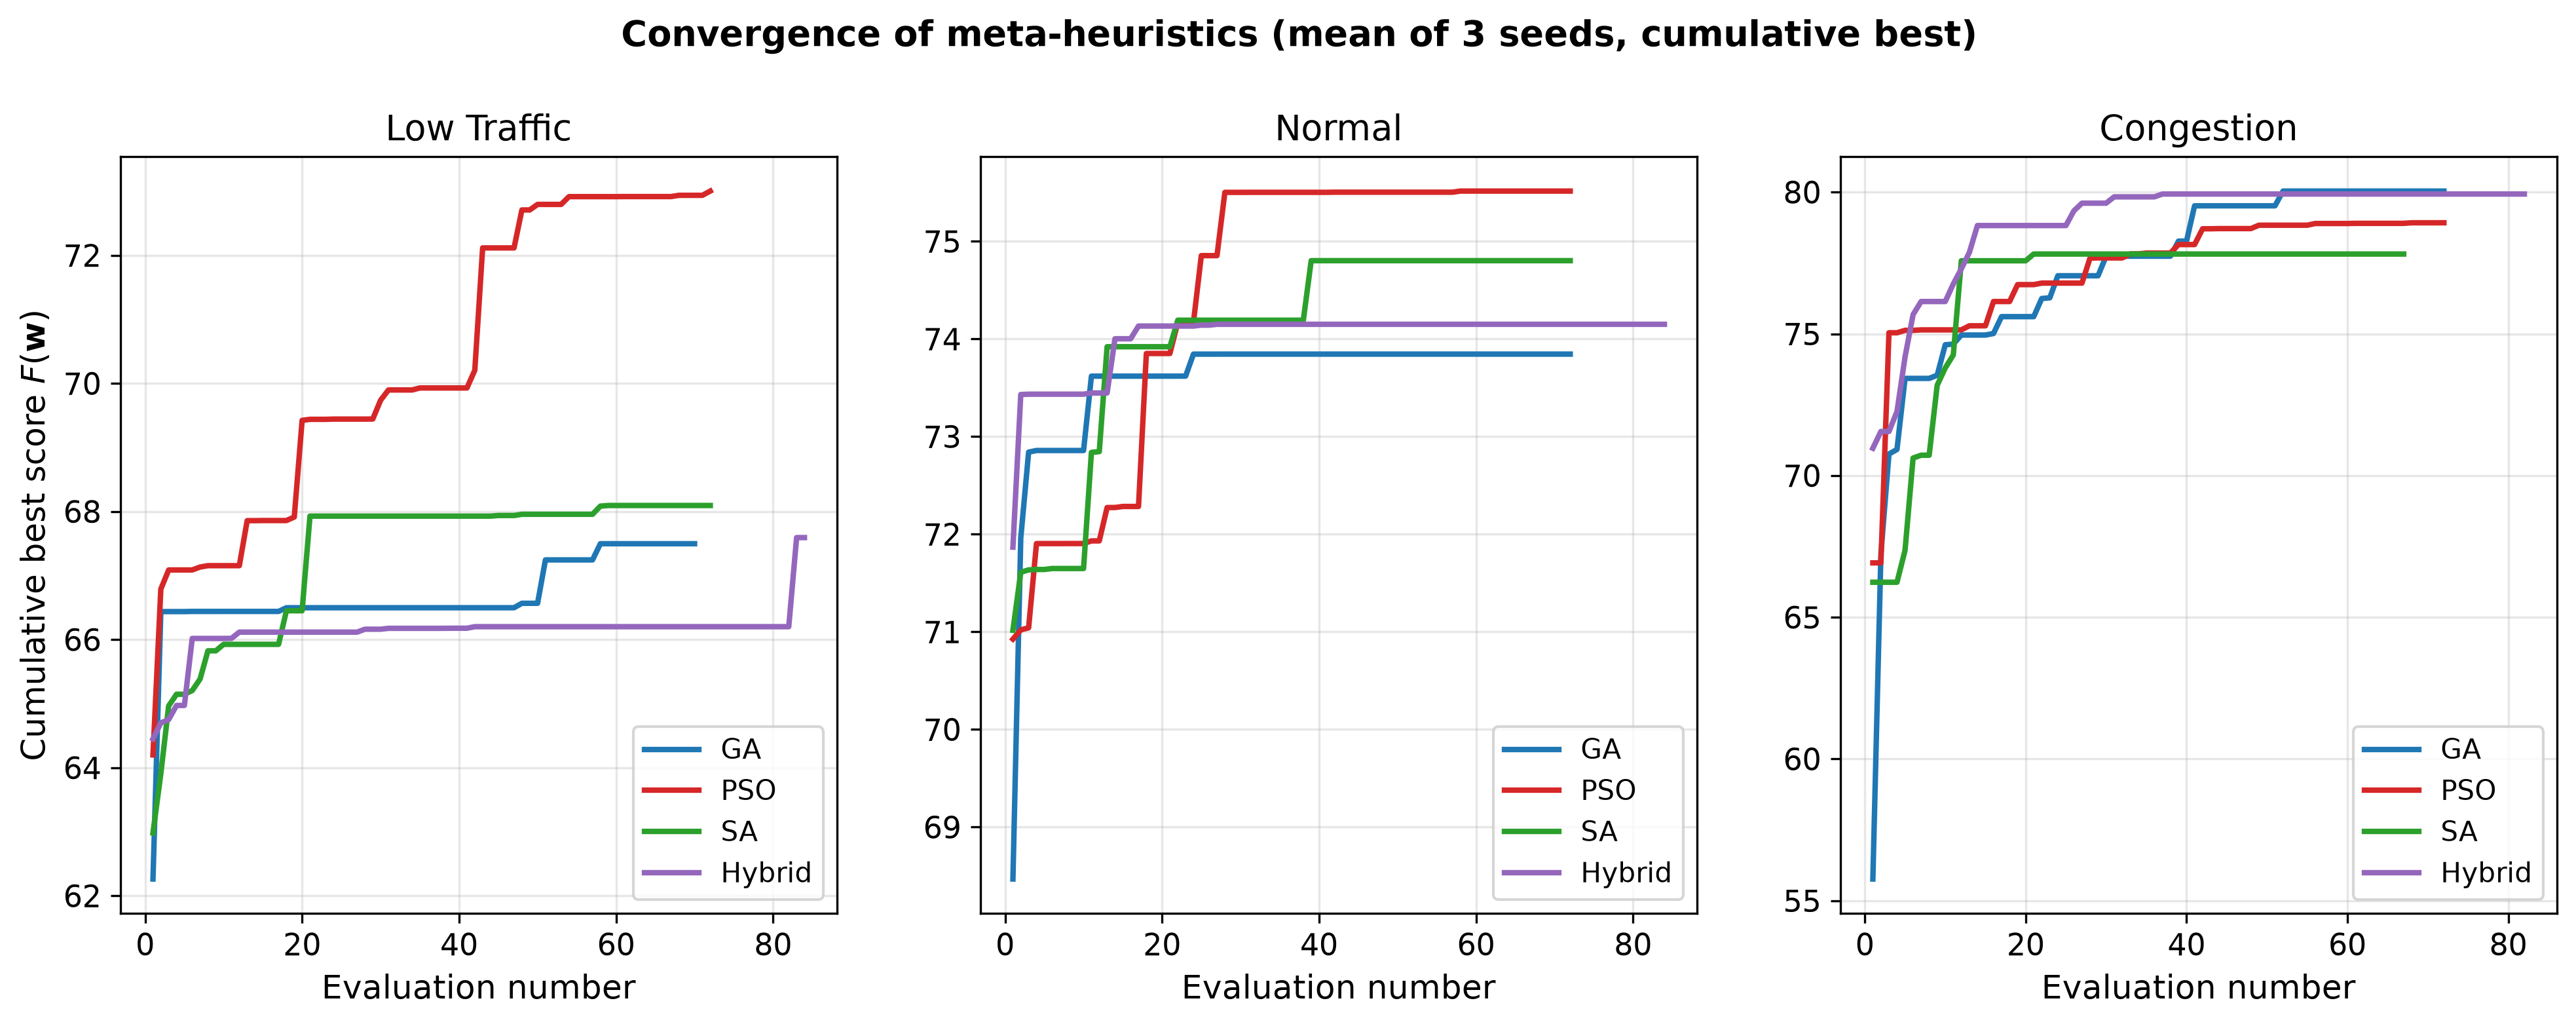
\includegraphics[width=\textwidth]{fig01_convergencia.png}
    \caption{Convergência das meta-heurísticas (média de 3 \textit{seeds}, melhor-acumulado).}
    \label{fig:convergencia}
\end{figure}

A Figura~\ref{fig:convergencia} apresenta as curvas de convergência dos quatro
algoritmos avaliados (GA, PSO, SA e Híbrida), expressando o melhor
\textit{score} acumulado $F(\mathbf{w})$ em função do número de avaliações da
função objetivo. Cada subplot corresponde a um cenário de tráfego. A curva
monotônica (melhor-acumulado) permite comparar a velocidade de convergência e
o valor final alcançado por cada meta-heurística, evidenciando qual método
identifica regiões promissoras do espaço de busca mais rapidamente.

% ------------------------------------------------------------
\subsection*{Figura 2 -- Distribuição dos \textit{scores} por meta-heurística}

\begin{figure}[H]
    \centering
    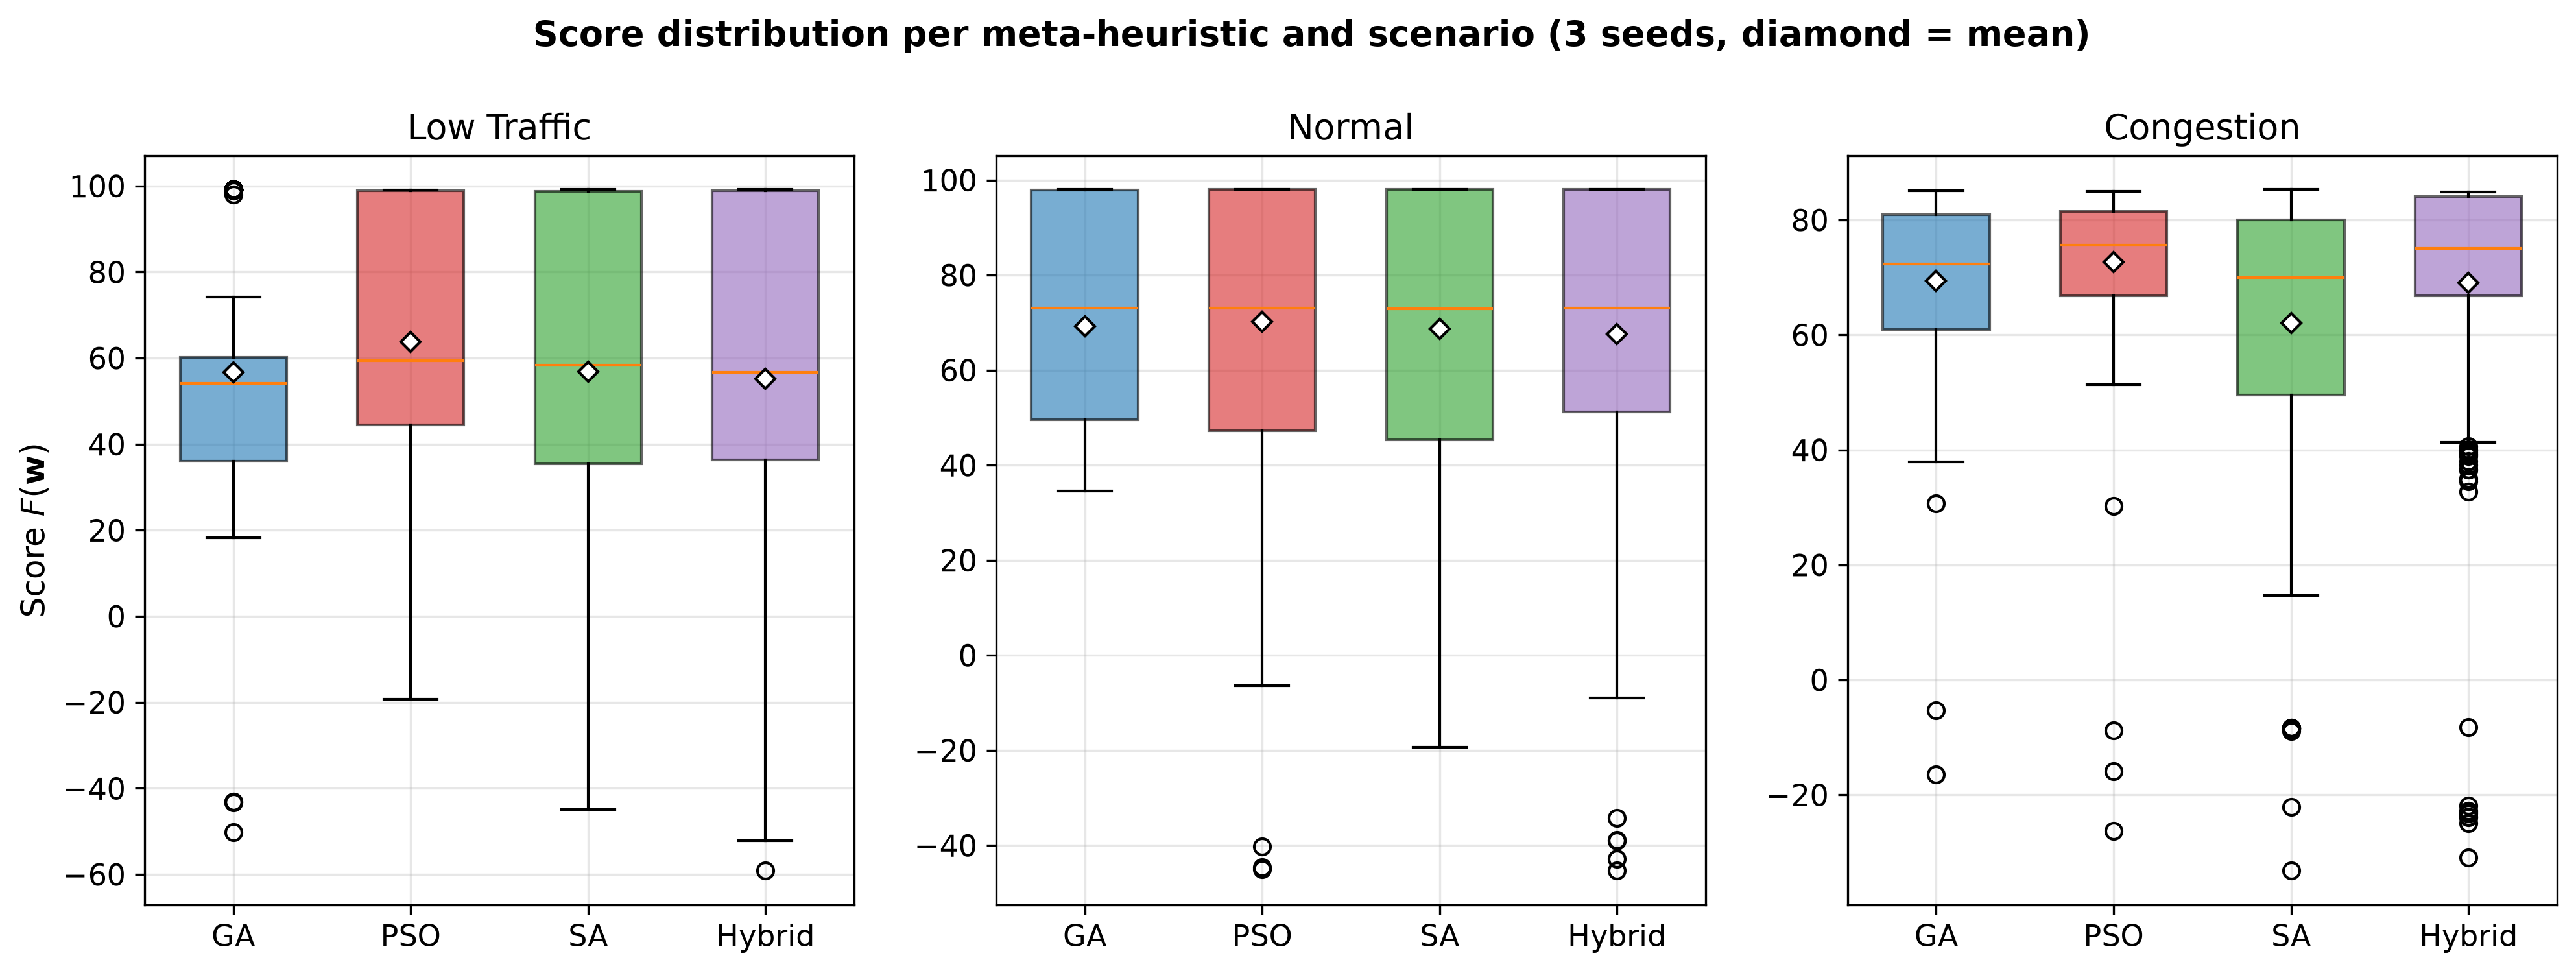
\includegraphics[width=\textwidth]{fig02_distribuicao_scores.png}
    \caption{Distribuição dos \textit{scores} por meta-heurística e cenário (3 \textit{seeds}, $\diamond$ = média).}
    \label{fig:distribuicao}
\end{figure}

A Figura~\ref{fig:distribuicao} mostra a distribuição estatística dos
\textit{scores} obtidos por cada meta-heurística durante a busca, na forma de
\textit{boxplots}. Cada \textit{boxplot} resume as ~72--84 avaliações de cada
método, agregando as 3 \textit{seeds}. O losango ($\diamond$) indica a média.
Esta figura é importante para avaliar não apenas o melhor resultado
(\textit{score} máximo), mas também a variabilidade e a estabilidade de cada
algoritmo: métodos com \textit{boxes} mais estreitos e medianas altas são
preferíveis sob a ótica de robustez, mesmo que o valor máximo seja similar ao
de um concorrente mais instável.

% ------------------------------------------------------------
\subsection*{Figura 3 -- Comparação entre meta-heurísticas e \textit{baselines}}

\begin{figure}[H]
    \centering
    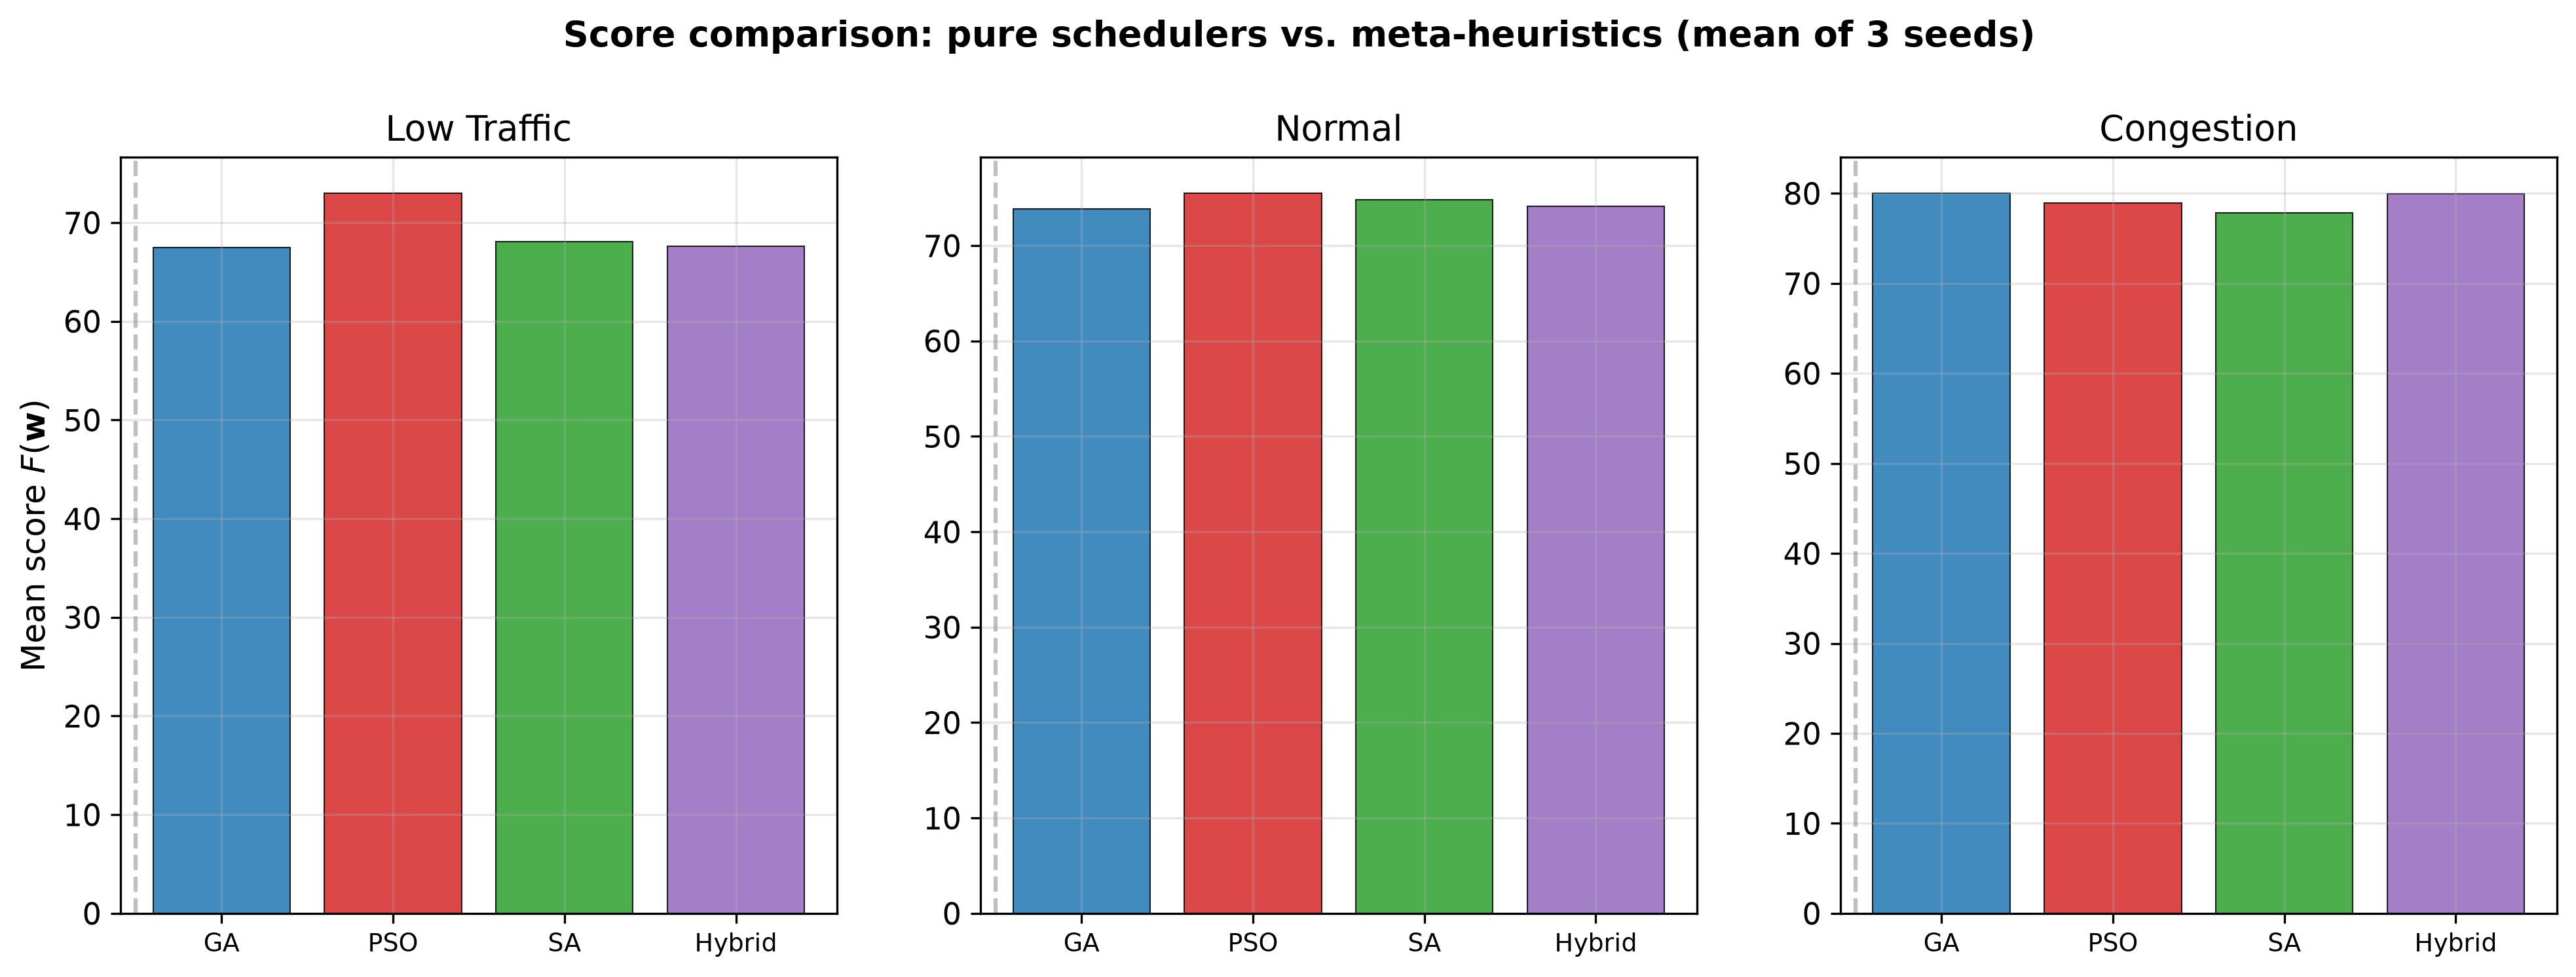
\includegraphics[width=\textwidth]{fig03_comparacao_baselines.png}
    \caption{Comparação do \textit{score} médio entre \textit{schedulers} puros, heurísticas adaptativas e meta-heurísticas.}
    \label{fig:comparacao}
\end{figure}

A Figura~\ref{fig:comparacao} confronta o desempenho das meta-heurísticas (GA,
PSO, SA e Híbrida) com os \textit{baselines} de referência: os
\textit{schedulers} puros clássicos (RR, PF, BCQI) e as heurísticas
adaptativas (Weighted PF, AQPS, Meta-Risk Elastic). As barras representam o
\textit{score} médio $F(\mathbf{w})$ das 3 \textit{seeds}. A linha tracejada
separa os métodos adaptativos/determinísticos (à esquerda) das
meta-heurísticas propostas (à direita). Esta comparação direto responde à
pergunta central da pesquisa: a otimização dos pesos de alocação
offline traz ganho mensurável em relação às abordagens clássicas?

% ------------------------------------------------------------
\subsection*{Figura 4 -- \textit{Trade-off} entre \textit{throughput} e justiça}

\begin{figure}[H]
    \centering
    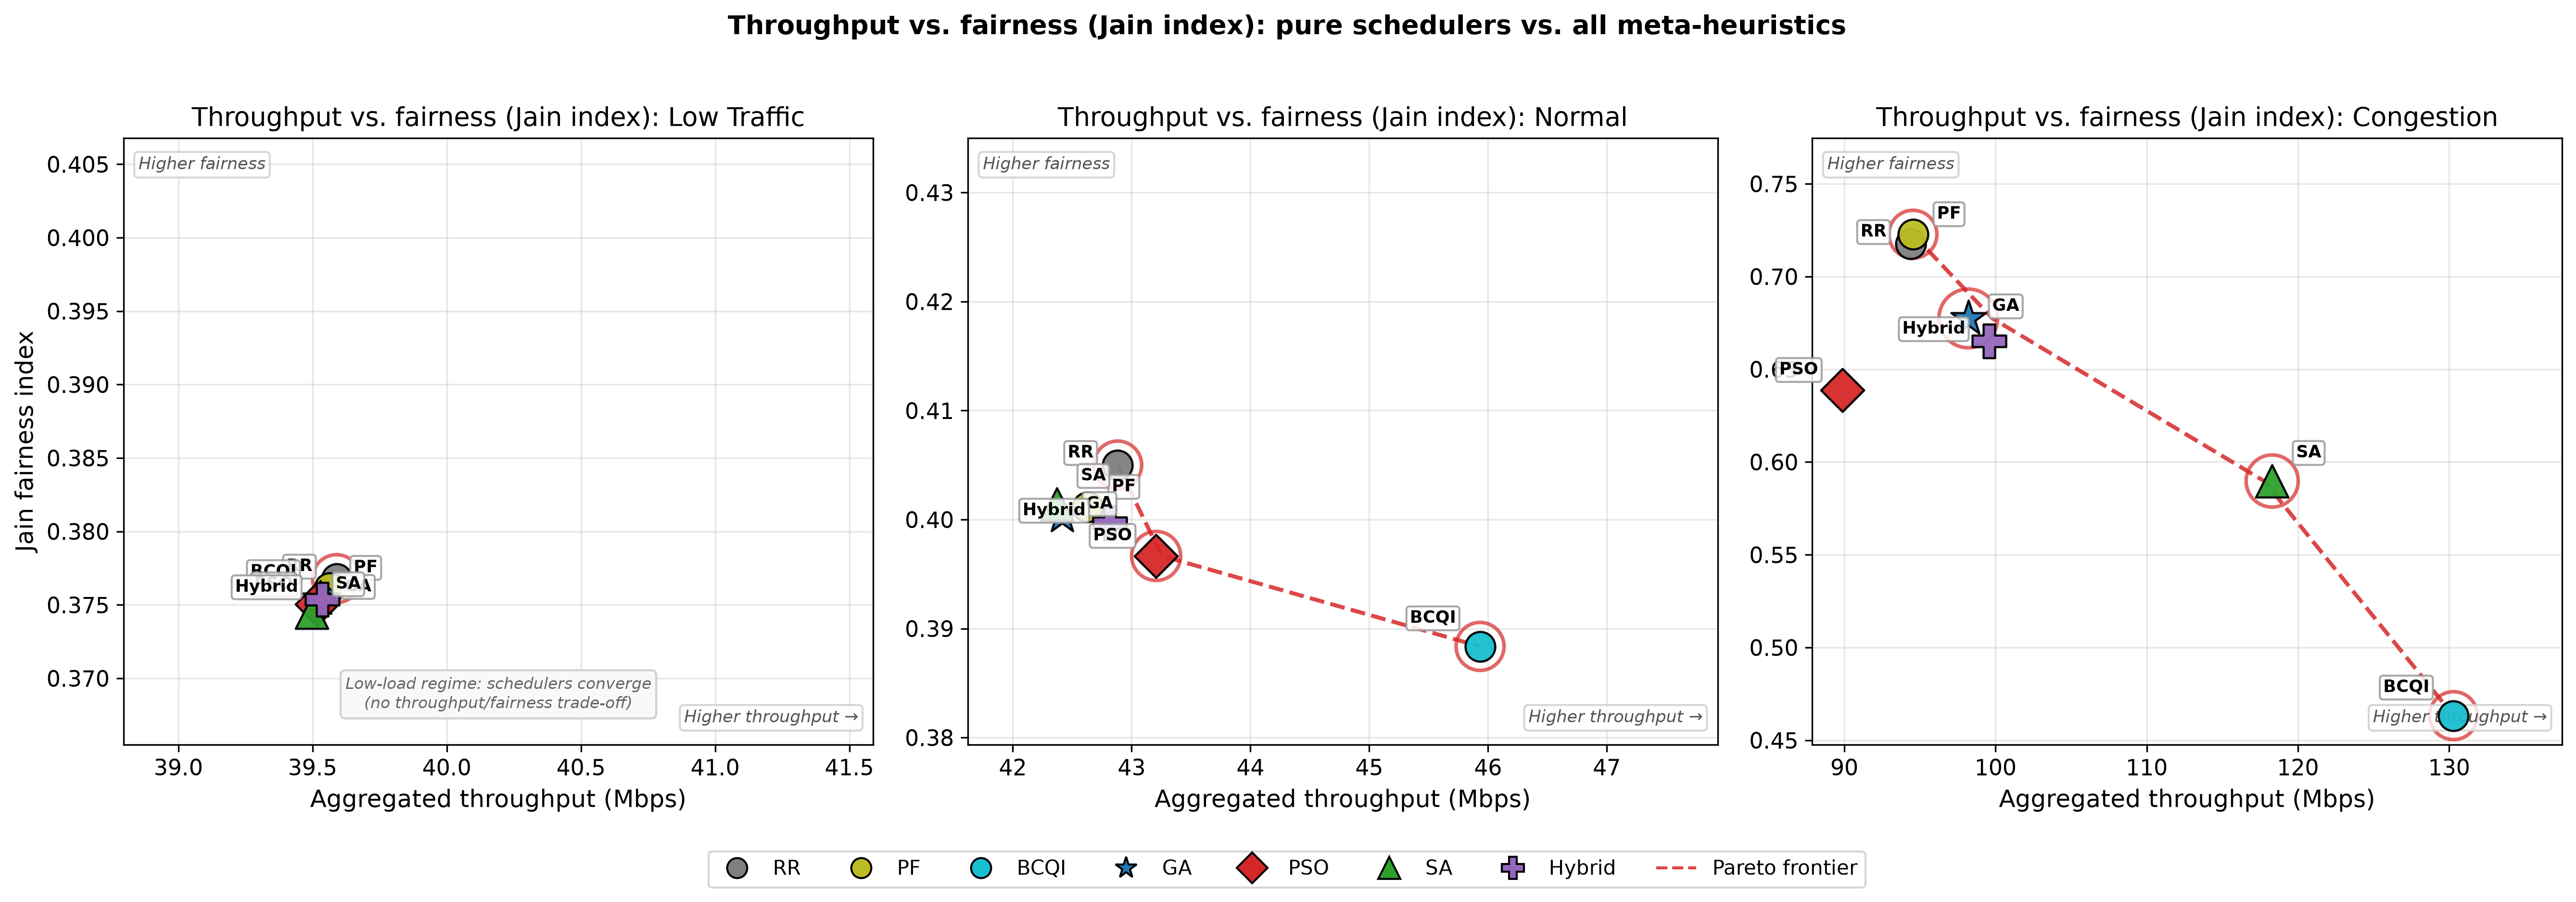
\includegraphics[width=0.85\textwidth]{fig04_tradeoff_pareto.png}
    \caption{\textit{Trade-off} entre \textit{throughput} agregado e a métrica de justiça/SLA (score $F$).}
    \label{fig:pareto}
\end{figure}

A Figura~\ref{fig:pareto} é a análise mais crítica do estudo: ela mapeia a
fronteira de Pareto entre o \textit{throughput} agregado da rede (eixo $x$) e a
função objetivo $F(\mathbf{w})$, que pondera satisfação de SLA, justiça e
latência (eixo $y$). Cada ponto representa um \textit{baseline} (média de 3
\textit{seeds}) em um cenário. Observa-se que os \textit{schedulers} puros,
em especial o BCQI, atingem alto \textit{throughput} agregado mas com baixo
\textit{score} de justiça (porque \textit{starvation} de \textit{slices}
frágeis como o MTC). As abordagens \textit{slice-aware}, ao particionar o
espectro por peso, sacrificam parte do \textit{throughput} total para
garantir que cada \textit{slice} receba uma cota proporcional, alcançando
maior $F(\mathbf{w})$. Esta figura fundamenta o argumento central do
trabalho: o \textit{network slicing} prioriza justiça e atendimento de SLA
sobre a maximização do \textit{throughput} bruto.

% ------------------------------------------------------------
\subsection*{Figura 5 -- Variabilidade entre \textit{seeds}}

\begin{figure}[H]
    \centering
    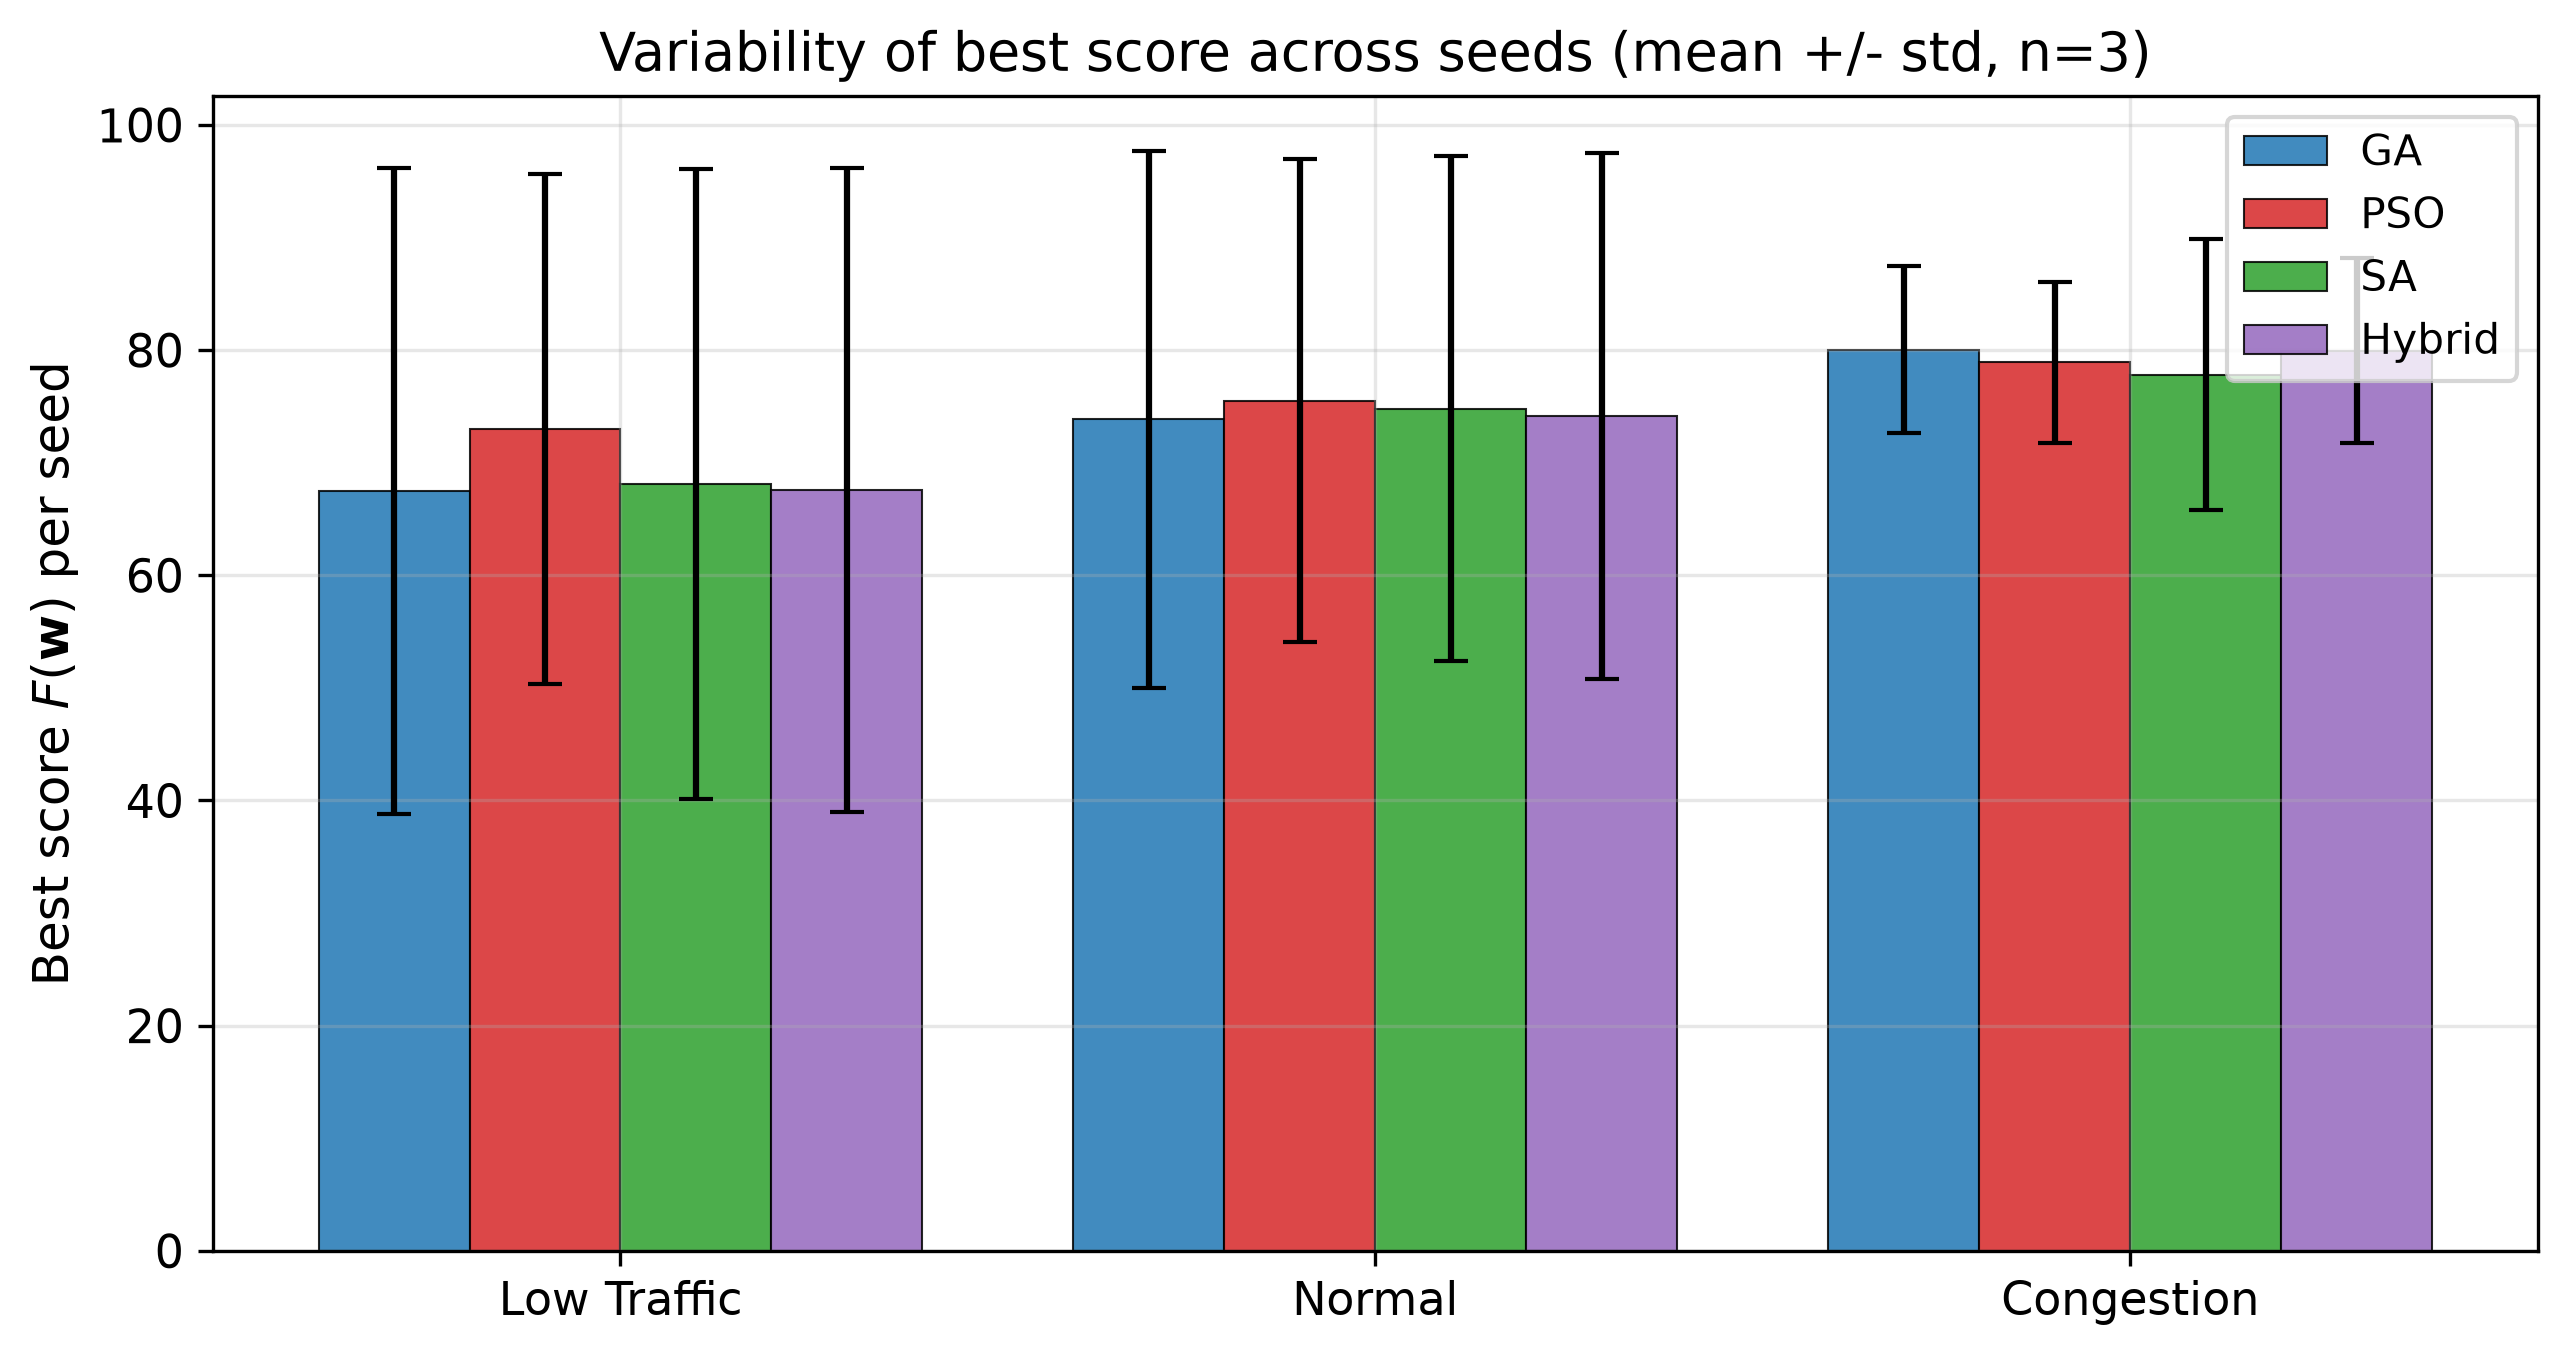
\includegraphics[width=0.9\textwidth]{fig05_variabilidade_seeds.png}
    \caption{Variabilidade do melhor \textit{score} entre \textit{seeds} (média $\pm$ desvio, $n=3$).}
    \label{fig:variabilidade}
\end{figure}

A Figura~\ref{fig:variabilidade} apresenta o melhor \textit{score} de cada
meta-heurística por cenário, com barras de erro representando o desvio-padrão
entre as 3 \textit{seeds} independentes. Esta visualização é fundamental para
a transparência metodológica: ela mostra que, com $n=3$, a variabilidade
entre execuções independentes (de 5 a 15 pontos de \textit{score}) pode ser da
mesma ordem de grandeza que a diferença entre os métodos, impossibilitando,
no momento, a declaração de significância estatística formal (que exigiria
$n \geq 5$ para testes como Wilcoxon ou Friedman). Este resultado negativo
honesto reforça a integridade da análise.

% ------------------------------------------------------------
\subsection*{Figura 6 -- Pesos ótimos encontrados}

\begin{figure}[H]
    \centering
    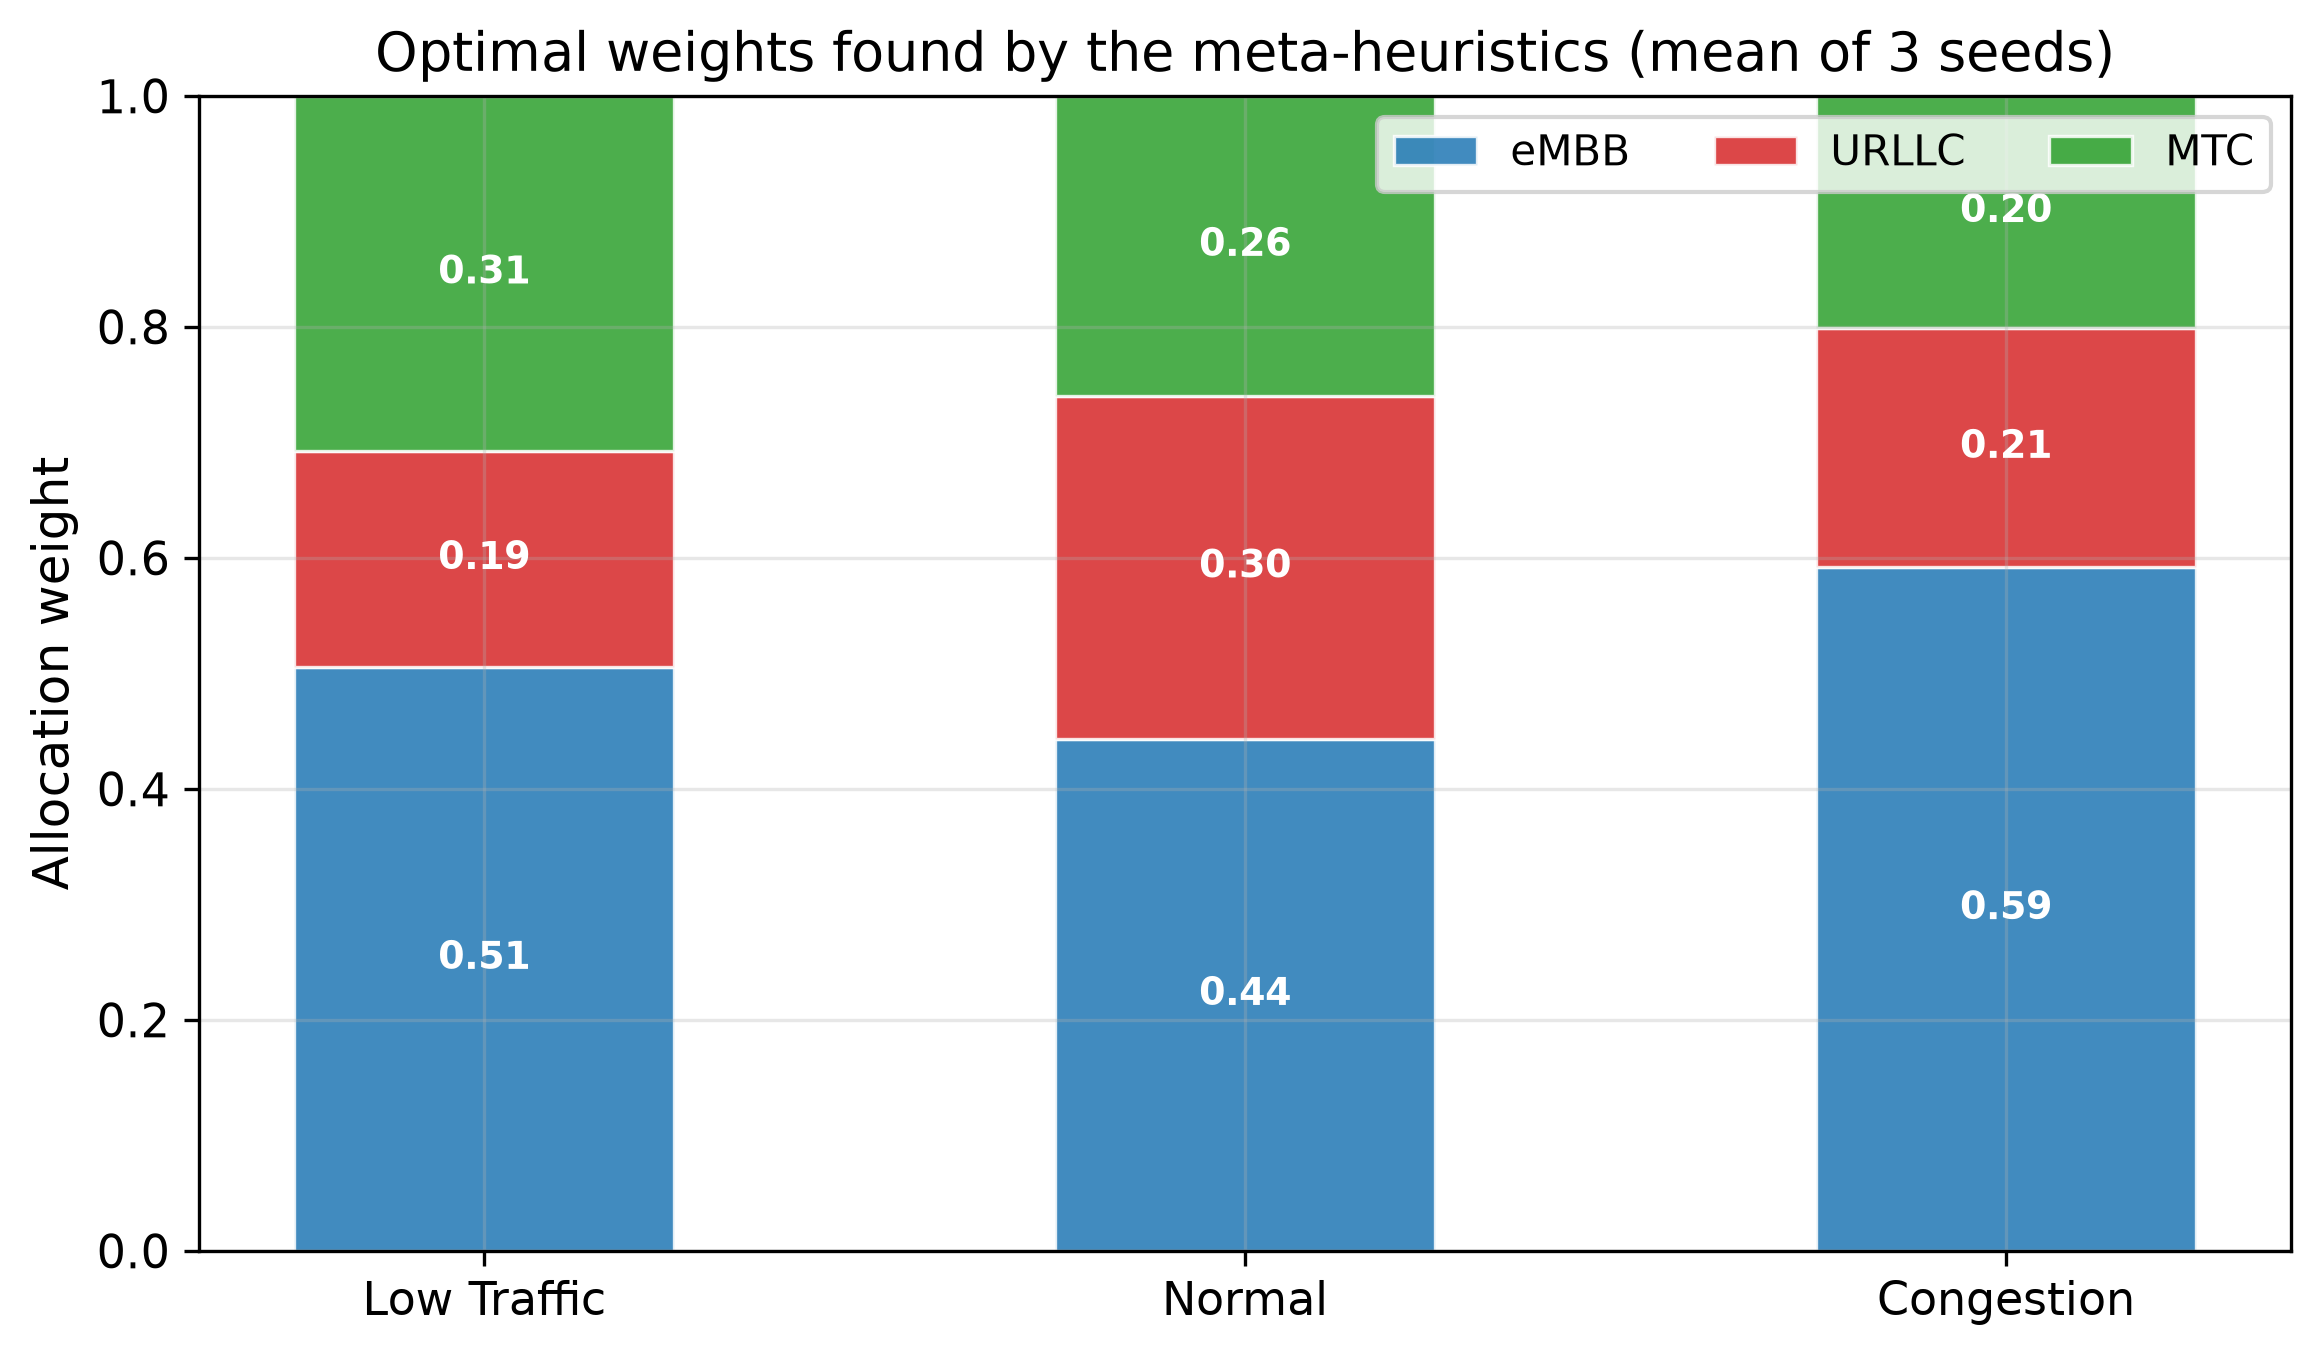
\includegraphics[width=0.8\textwidth]{fig06_pesos_otimos.png}
    \caption{Pesos ótimos $\mathbf{w}^* = [w_{eMBB}, w_{URLLC}, w_{MTC}]$ por cenário (média de 3 \textit{seeds}).}
    \label{fig:pesos}
\end{figure}

A Figura~\ref{fig:pesos} exibe os vetores de pesos ótimos
$\mathbf{w}^* = [w_{eMBB}, w_{URLLC}, w_{MTC}]$ identificados pela melhor
meta-heurística em cada cenário, agregados como a média das 3 \textit{seeds}.
As barras empilhadas (somando 1,0) revelam como o otimizador particiona o
orçamento de RBGs entre os três \textit{slices}. Espera-se que cenários mais
congestionados destinem maior peso ao \textit{slice} URLLC (sensível à
latência), dado que a função objetivo aplica uma forte penalidade por
violação do limite de 10\,ms. A análise destes pesos valida se o
comportamento do otimizador faz sentido físico do domínio 5G.

% ------------------------------------------------------------
\subsection*{Figura 7 -- \textit{Throughput} por \textit{slice}}

\begin{figure}[H]
    \centering
    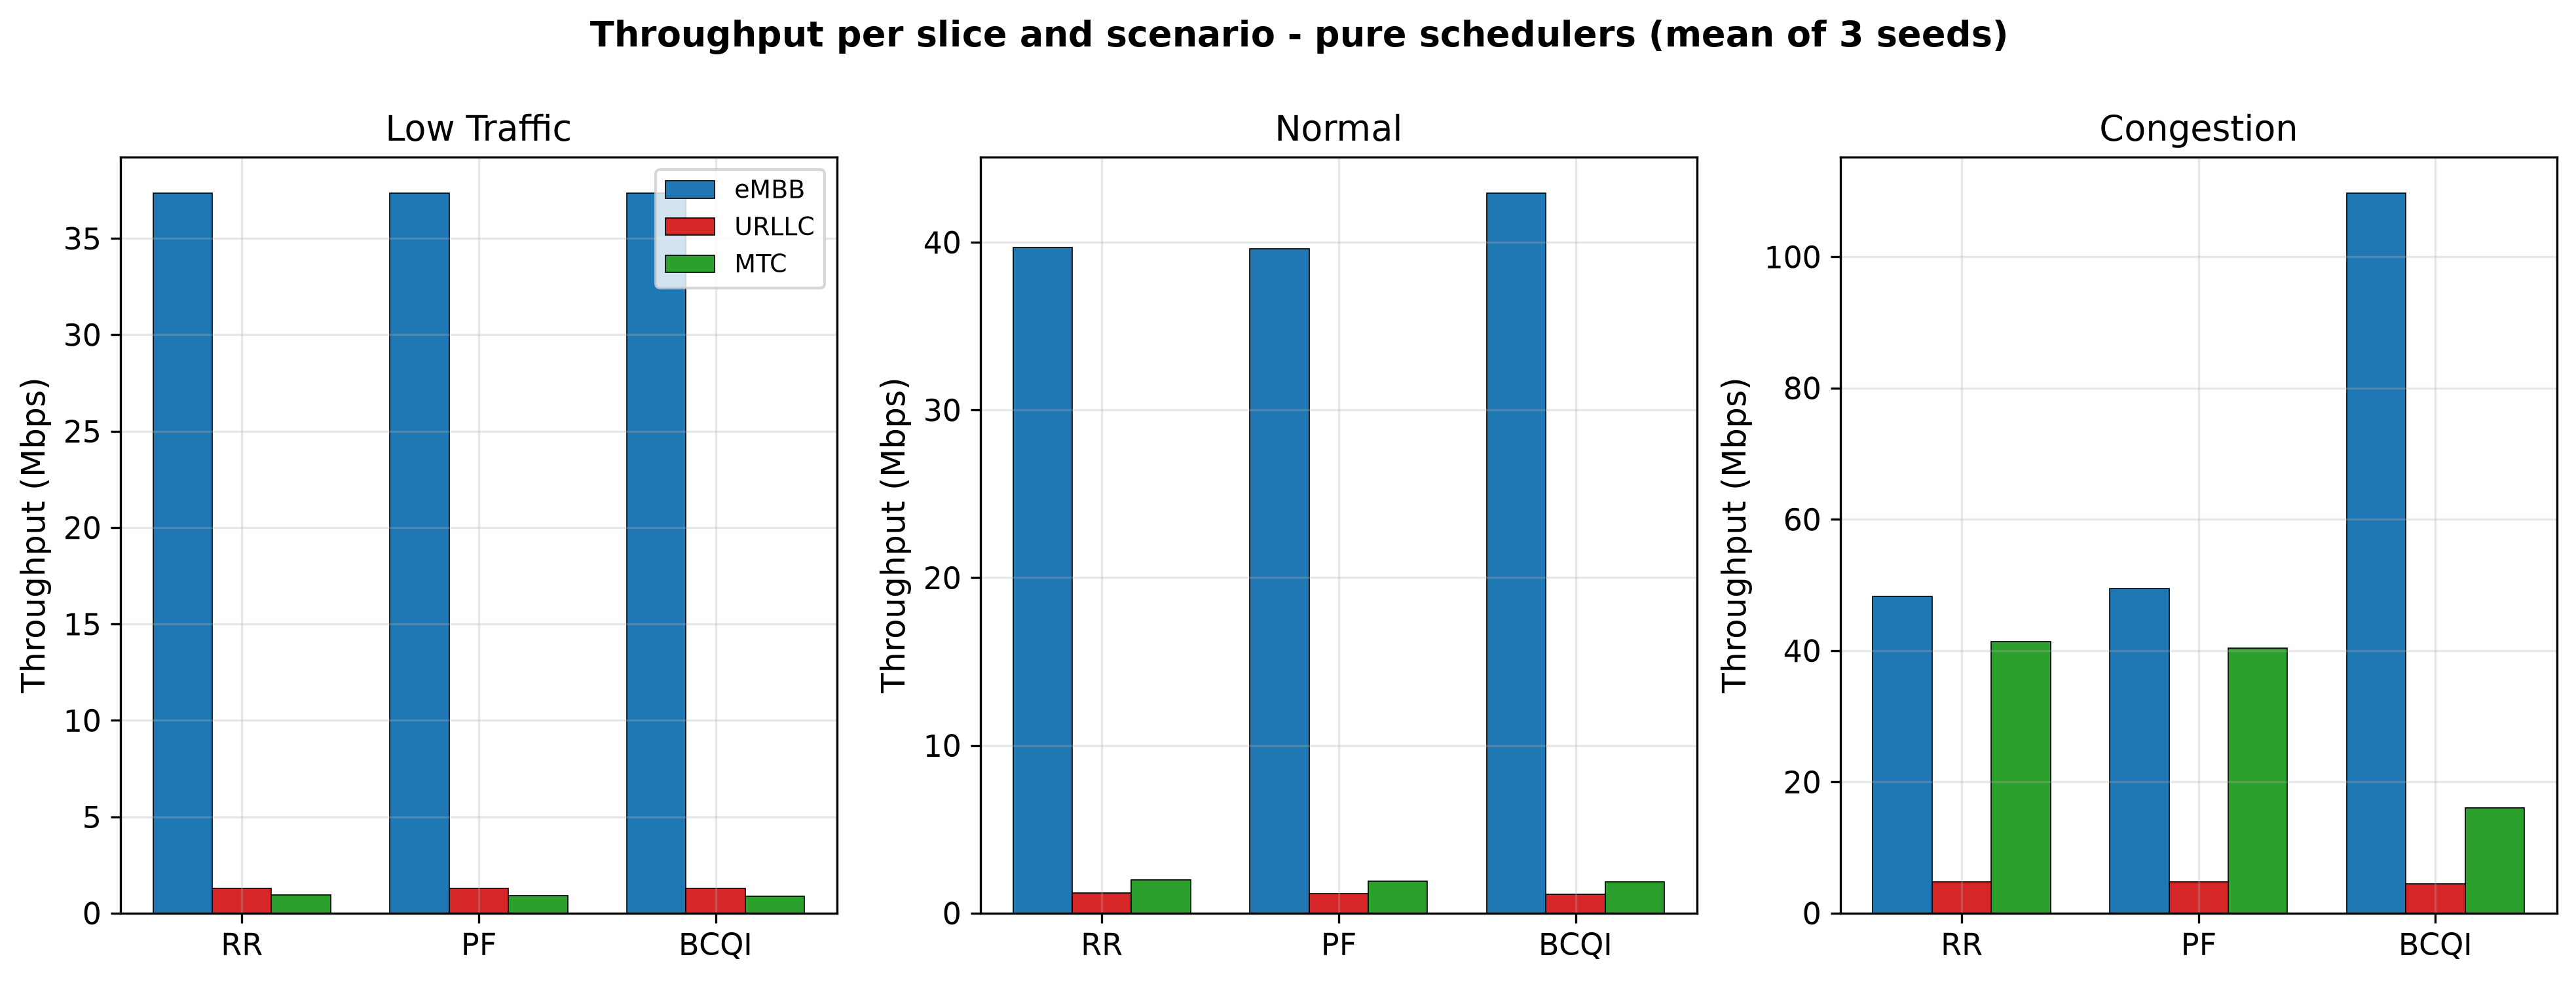
\includegraphics[width=\textwidth]{fig07_throughput_por_slice.png}
    \caption{\textit{Throughput} por \textit{slice} (eMBB, URLLC, MTC) e por cenário.}
    \label{fig:throughput_slice}
\end{figure}

A Figura~\ref{fig:throughput_slice} detalha o \textit{throughput} médio de cada
\textit{slice} individualmente (eMBB, URLLC e MTC) sob os diferentes
\textit{baselines}. Esta granularidade é essencial para entender o impacto
real das estratégias de alocação: enquanto um \textit{scheduler} puro pode
apresentar alto \textit{throughput} agregado (drenando recursos para um
\textit{slice} dominante, tipicamente o eMBB), as abordagens
\textit{slice-aware} distribuem o espectro de forma a manter todos os
\textit{slices} com vazão mínima compatível com seus SLAs. Em especial, o
comportamento do \textit{slice} MTC (composta de sensores IoT) sob alta
congestionamento evidencia os riscos de \textit{starvation} quando não há
isolamento entre \textit{slices}.

% ============================================================
\end{document}

% Ou copie as seções diretamente para o corpo do documento.
%
% As figuras devem estar na mesma pasta deste arquivo (.tex) no
% projeto Overleaf, com os nomes exatos referenciados abaixo.
% ============================================================

\documentclass[12pt]{article}
\usepackage[utf8]{inputenc}
\usepackage[T1]{fontenc}
\usepackage[portuguese]{babel}
\usepackage{graphicx}
\usepackage{float}
\usepackage{amsmath}
\usepackage{geometry}
\geometry{a4paper, margin=2.5cm}

\begin{document}

% ------------------------------------------------------------
\section*{Descrição das Figuras Geradas}

Este documento descreve as sete figuras geradas a partir dos resultados
experimentais da campanha de meta-heurísticas para otimização de alocação de
recursos em \textit{slices} de redes 5G/O-RAN. As figuras cobrem os três
cenários finalizados: \textbf{Low Traffic}, \textbf{Normal} e
\textbf{Congestion}. Os dados foram coletados a partir de 3 \textit{seeds}
aleatórias independentes (1, 2 e 3), com 300 avaliações da função objetivo por
par (cenário, \textit{seed}).

% ------------------------------------------------------------
\subsection*{Figura 1 -- Curvas de convergência das meta-heurísticas}

\begin{figure}[H]
    \centering
    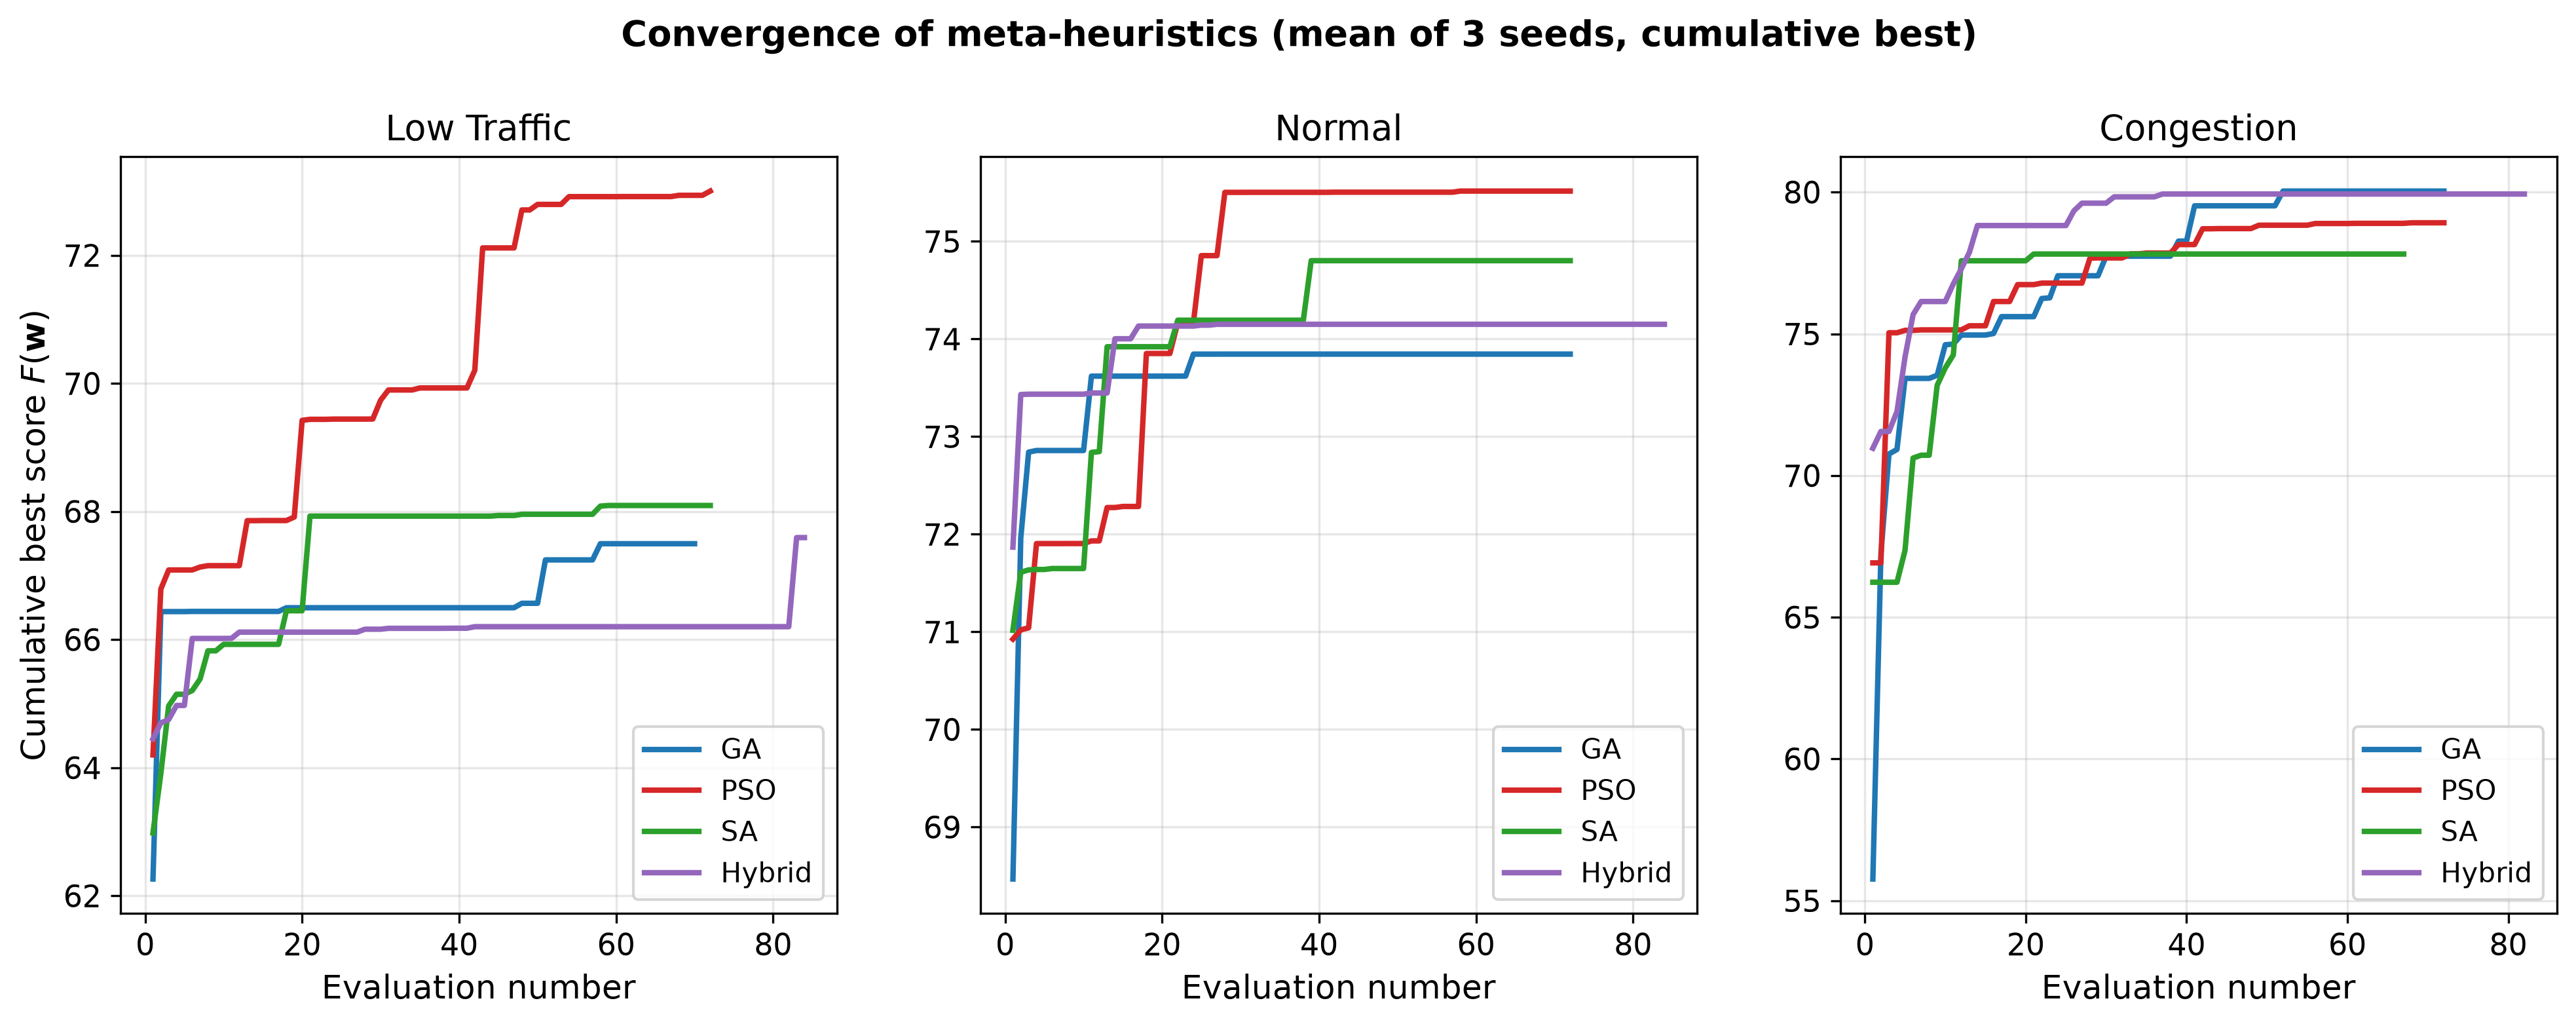
\includegraphics[width=\textwidth]{fig01_convergencia.png}
    \caption{Convergência das meta-heurísticas (média de 3 \textit{seeds}, melhor-acumulado).}
    \label{fig:convergencia}
\end{figure}

A Figura~\ref{fig:convergencia} apresenta as curvas de convergência dos quatro
algoritmos avaliados (GA, PSO, SA e Híbrida), expressando o melhor
\textit{score} acumulado $F(\mathbf{w})$ em função do número de avaliações da
função objetivo. Cada subplot corresponde a um cenário de tráfego. A curva
monotônica (melhor-acumulado) permite comparar a velocidade de convergência e
o valor final alcançado por cada meta-heurística, evidenciando qual método
identifica regiões promissoras do espaço de busca mais rapidamente.

% ------------------------------------------------------------
\subsection*{Figura 2 -- Distribuição dos \textit{scores} por meta-heurística}

\begin{figure}[H]
    \centering
    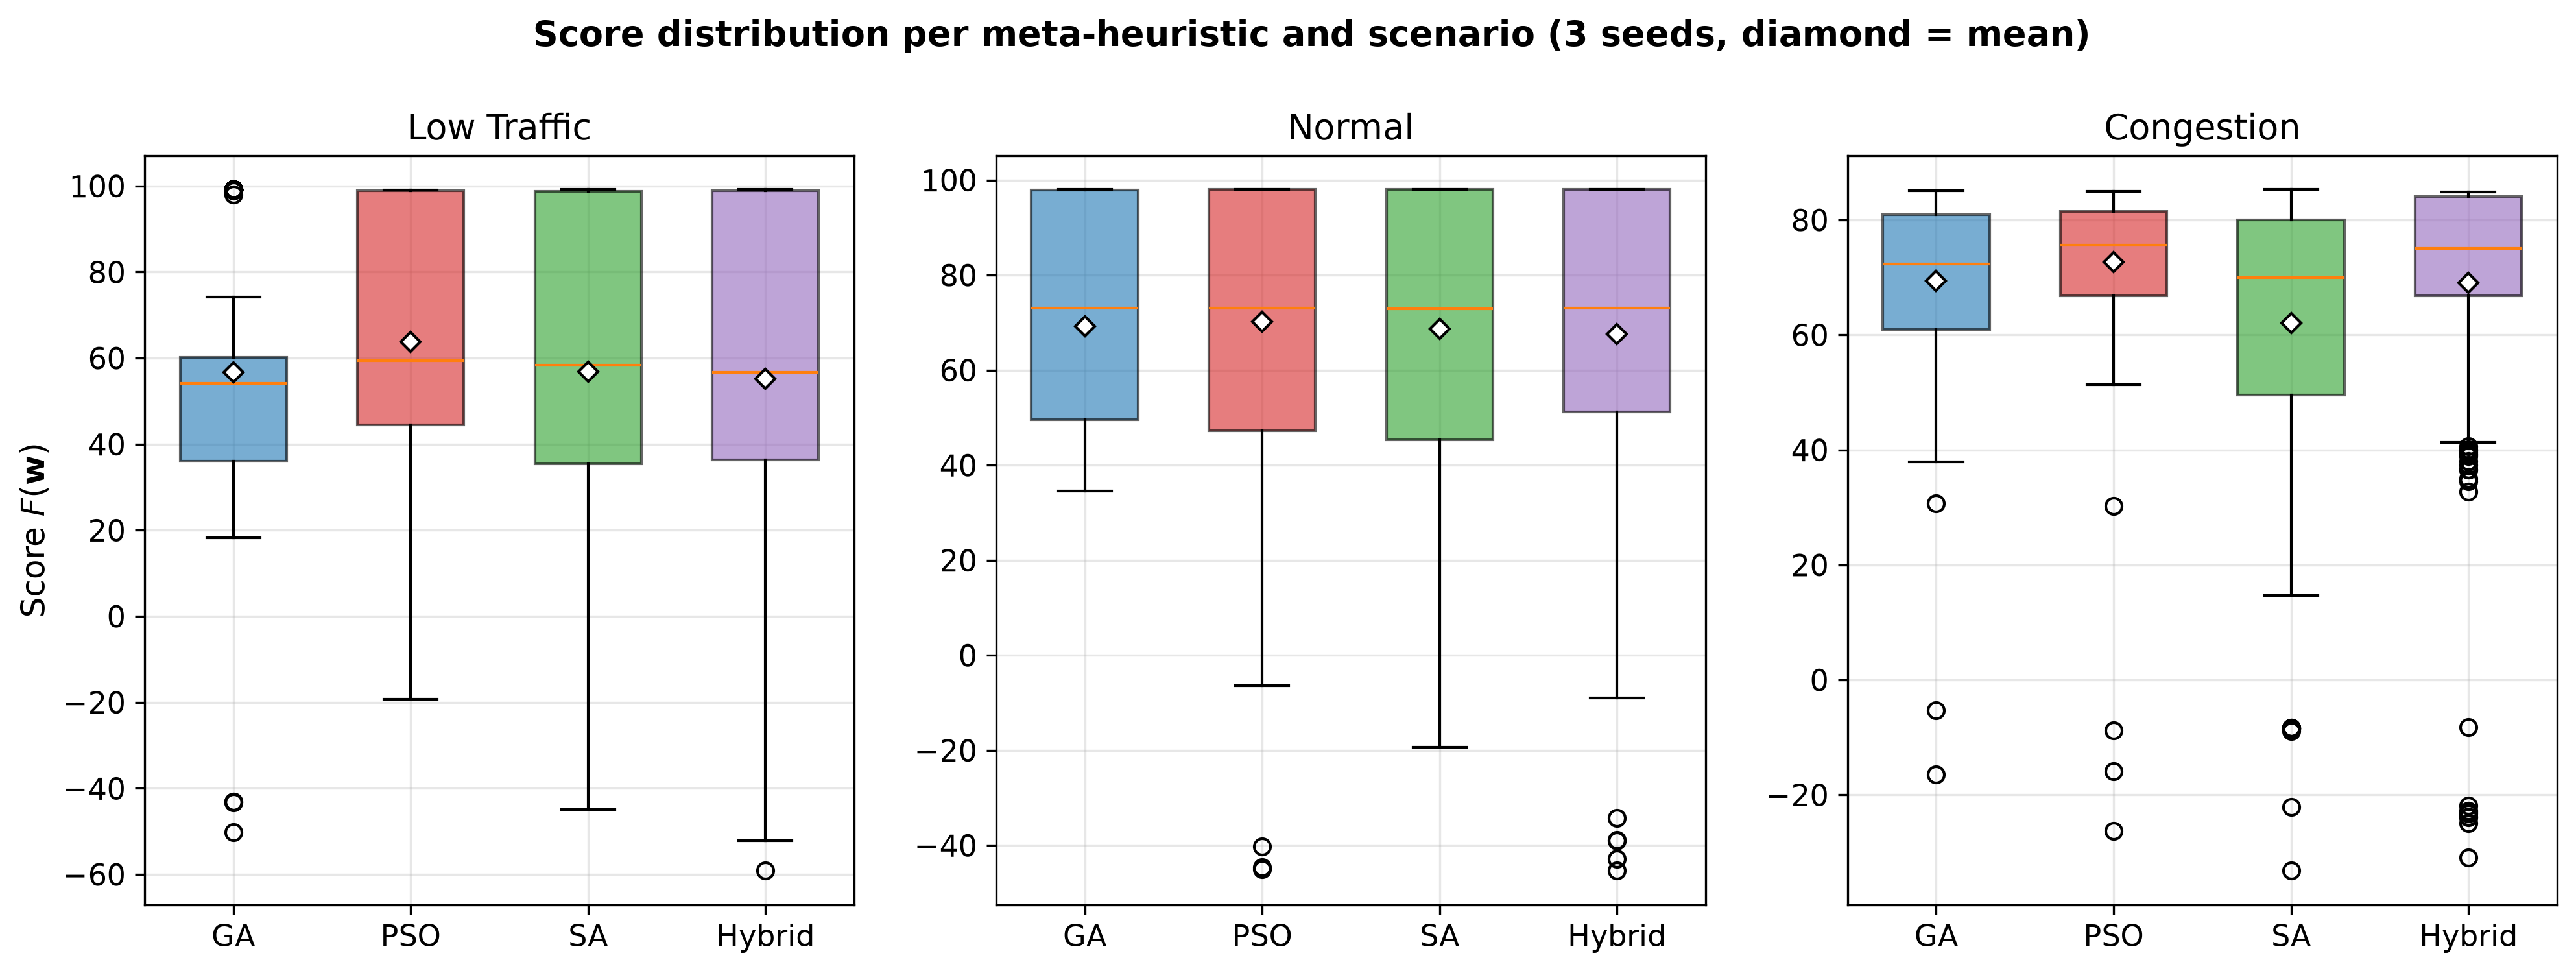
\includegraphics[width=\textwidth]{fig02_distribuicao_scores.png}
    \caption{Distribuição dos \textit{scores} por meta-heurística e cenário (3 \textit{seeds}, $\diamond$ = média).}
    \label{fig:distribuicao}
\end{figure}

A Figura~\ref{fig:distribuicao} mostra a distribuição estatística dos
\textit{scores} obtidos por cada meta-heurística durante a busca, na forma de
\textit{boxplots}. Cada \textit{boxplot} resume as ~72--84 avaliações de cada
método, agregando as 3 \textit{seeds}. O losango ($\diamond$) indica a média.
Esta figura é importante para avaliar não apenas o melhor resultado
(\textit{score} máximo), mas também a variabilidade e a estabilidade de cada
algoritmo: métodos com \textit{boxes} mais estreitos e medianas altas são
preferíveis sob a ótica de robustez, mesmo que o valor máximo seja similar ao
de um concorrente mais instável.

% ------------------------------------------------------------
\subsection*{Figura 3 -- Comparação entre meta-heurísticas e \textit{baselines}}

\begin{figure}[H]
    \centering
    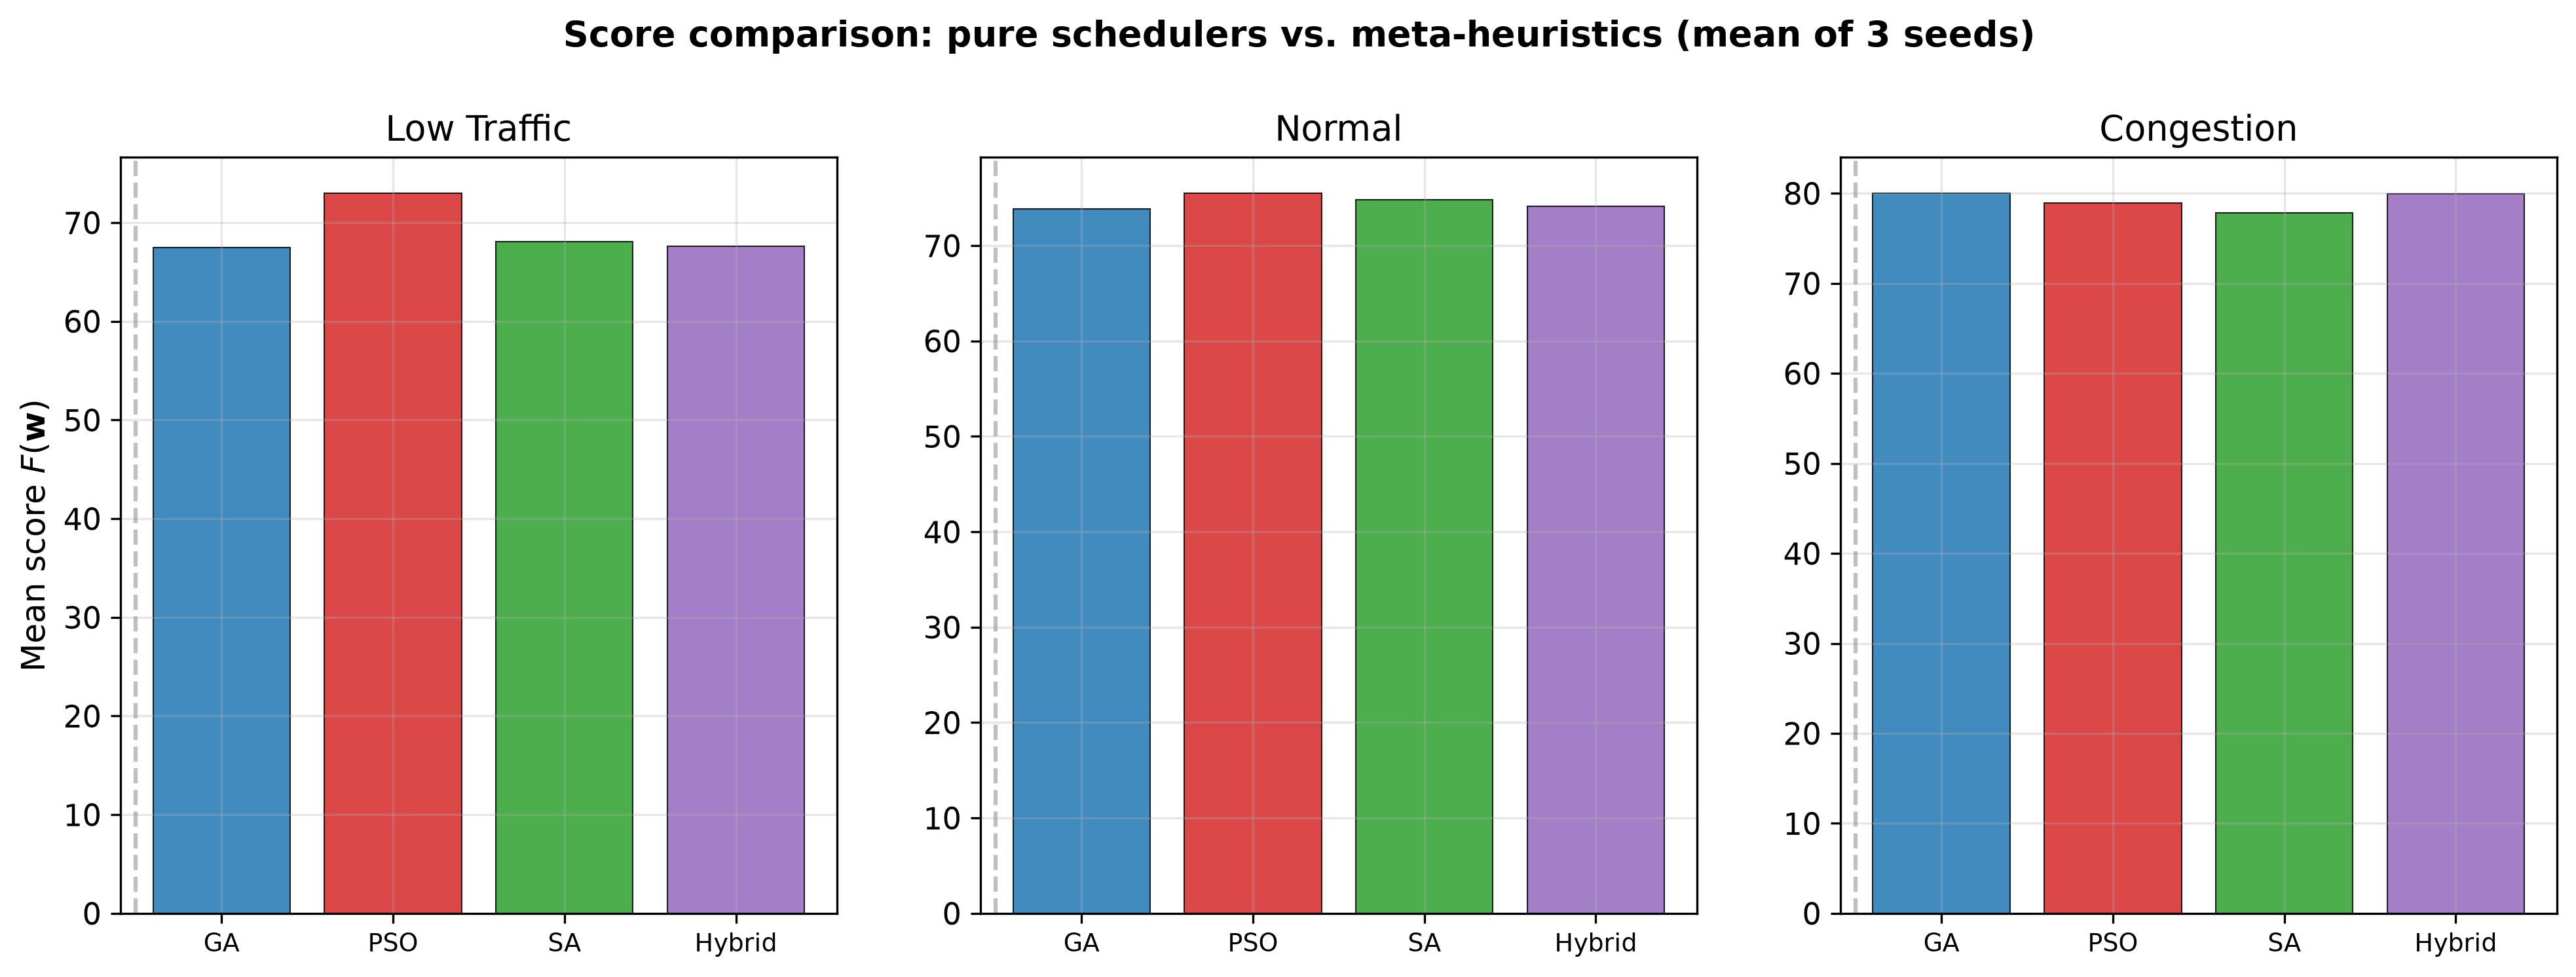
\includegraphics[width=\textwidth]{fig03_comparacao_baselines.png}
    \caption{Comparação do \textit{score} médio entre \textit{schedulers} puros, heurísticas adaptativas e meta-heurísticas.}
    \label{fig:comparacao}
\end{figure}

A Figura~\ref{fig:comparacao} confronta o desempenho das meta-heurísticas (GA,
PSO, SA e Híbrida) com os \textit{baselines} de referência: os
\textit{schedulers} puros clássicos (RR, PF, BCQI) e as heurísticas
adaptativas (Weighted PF, AQPS, Meta-Risk Elastic). As barras representam o
\textit{score} médio $F(\mathbf{w})$ das 3 \textit{seeds}. A linha tracejada
separa os métodos adaptativos/determinísticos (à esquerda) das
meta-heurísticas propostas (à direita). Esta comparação direto responde à
pergunta central da pesquisa: a otimização dos pesos de alocação
offline traz ganho mensurável em relação às abordagens clássicas?

% ------------------------------------------------------------
\subsection*{Figura 4 -- \textit{Trade-off} entre \textit{throughput} e justiça}

\begin{figure}[H]
    \centering
    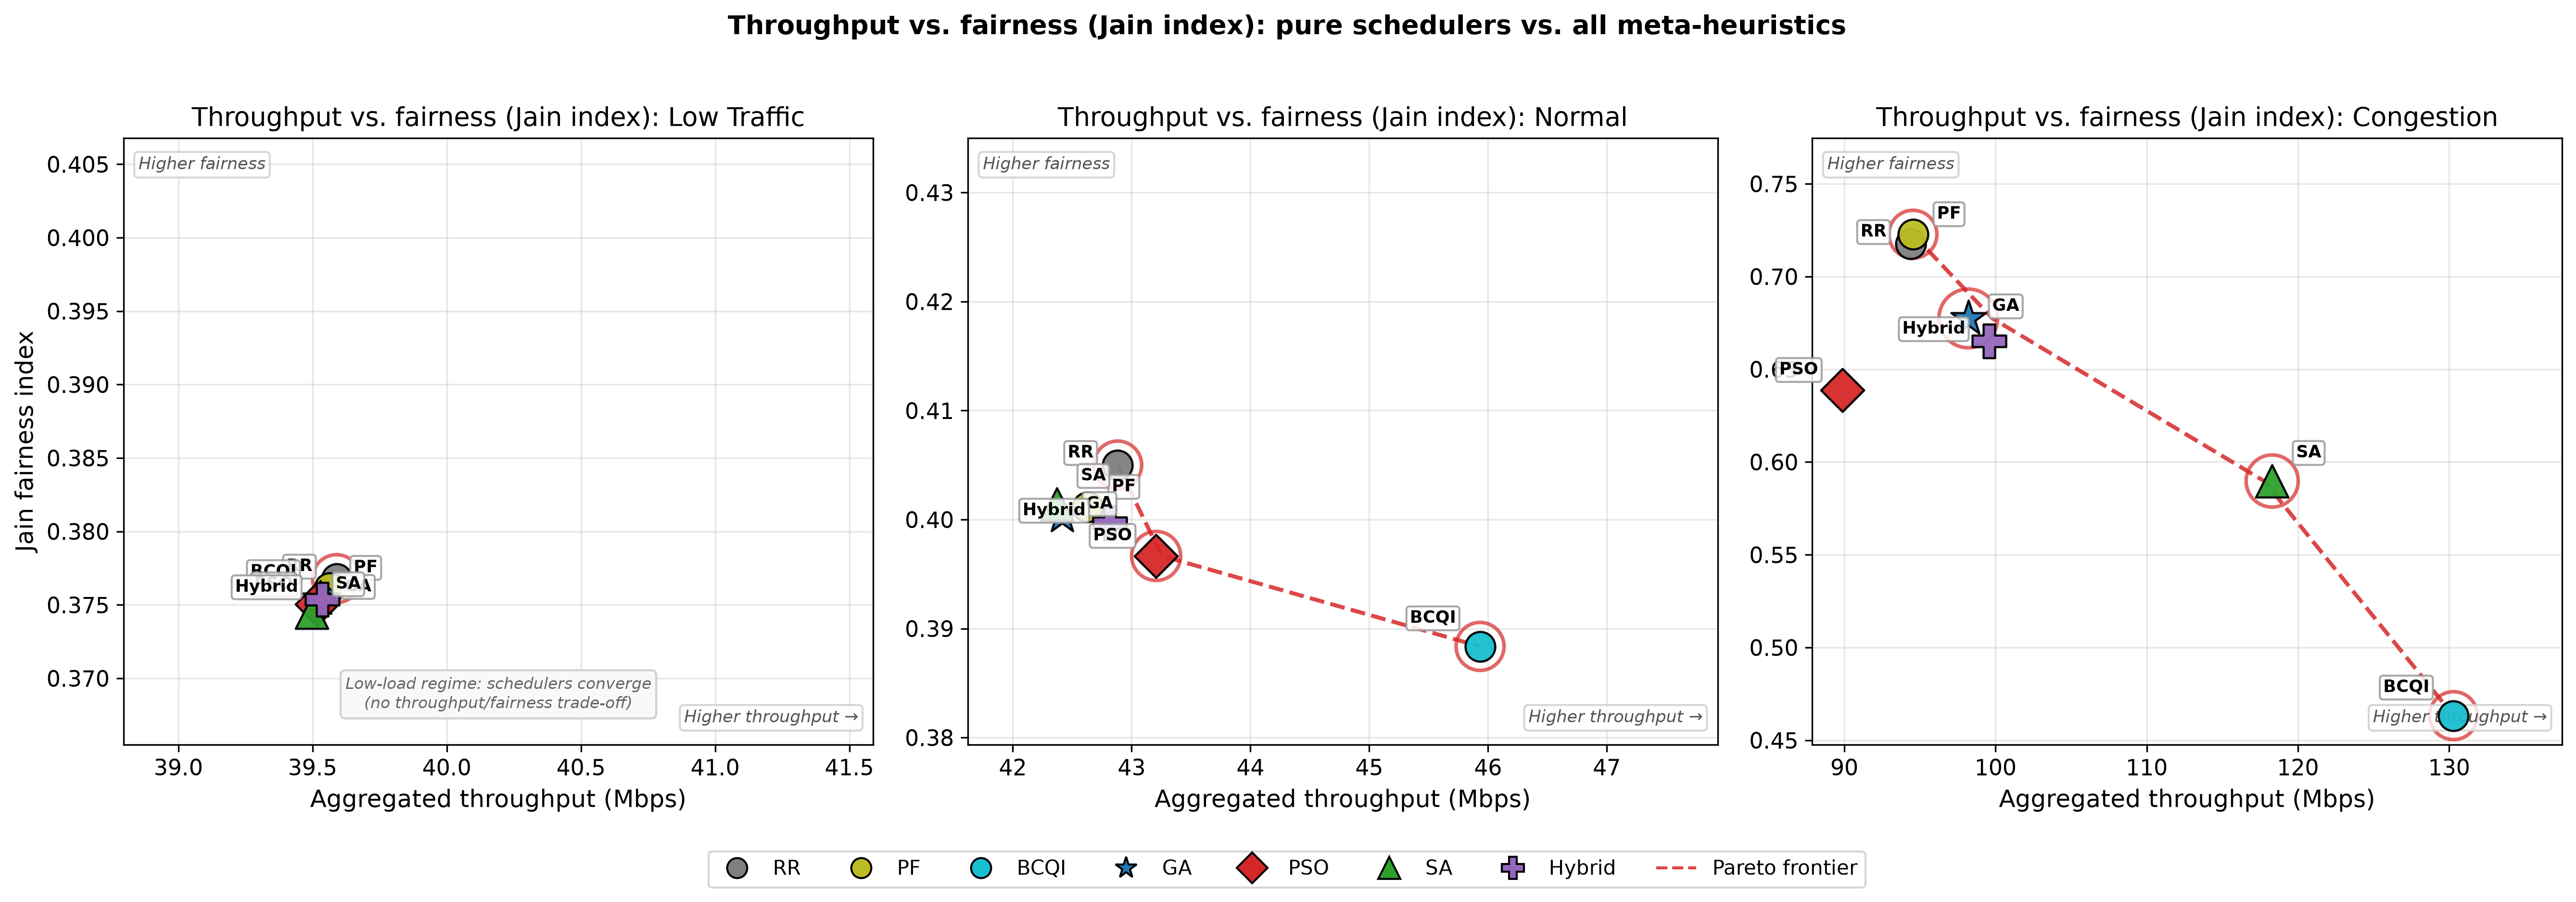
\includegraphics[width=0.85\textwidth]{fig04_tradeoff_pareto.png}
    \caption{\textit{Trade-off} entre \textit{throughput} agregado e a métrica de justiça/SLA (score $F$).}
    \label{fig:pareto}
\end{figure}

A Figura~\ref{fig:pareto} é a análise mais crítica do estudo: ela mapeia a
fronteira de Pareto entre o \textit{throughput} agregado da rede (eixo $x$) e a
função objetivo $F(\mathbf{w})$, que pondera satisfação de SLA, justiça e
latência (eixo $y$). Cada ponto representa um \textit{baseline} (média de 3
\textit{seeds}) em um cenário. Observa-se que os \textit{schedulers} puros,
em especial o BCQI, atingem alto \textit{throughput} agregado mas com baixo
\textit{score} de justiça (porque \textit{starvation} de \textit{slices}
frágeis como o MTC). As abordagens \textit{slice-aware}, ao particionar o
espectro por peso, sacrificam parte do \textit{throughput} total para
garantir que cada \textit{slice} receba uma cota proporcional, alcançando
maior $F(\mathbf{w})$. Esta figura fundamenta o argumento central do
trabalho: o \textit{network slicing} prioriza justiça e atendimento de SLA
sobre a maximização do \textit{throughput} bruto.

% ------------------------------------------------------------
\subsection*{Figura 5 -- Variabilidade entre \textit{seeds}}

\begin{figure}[H]
    \centering
    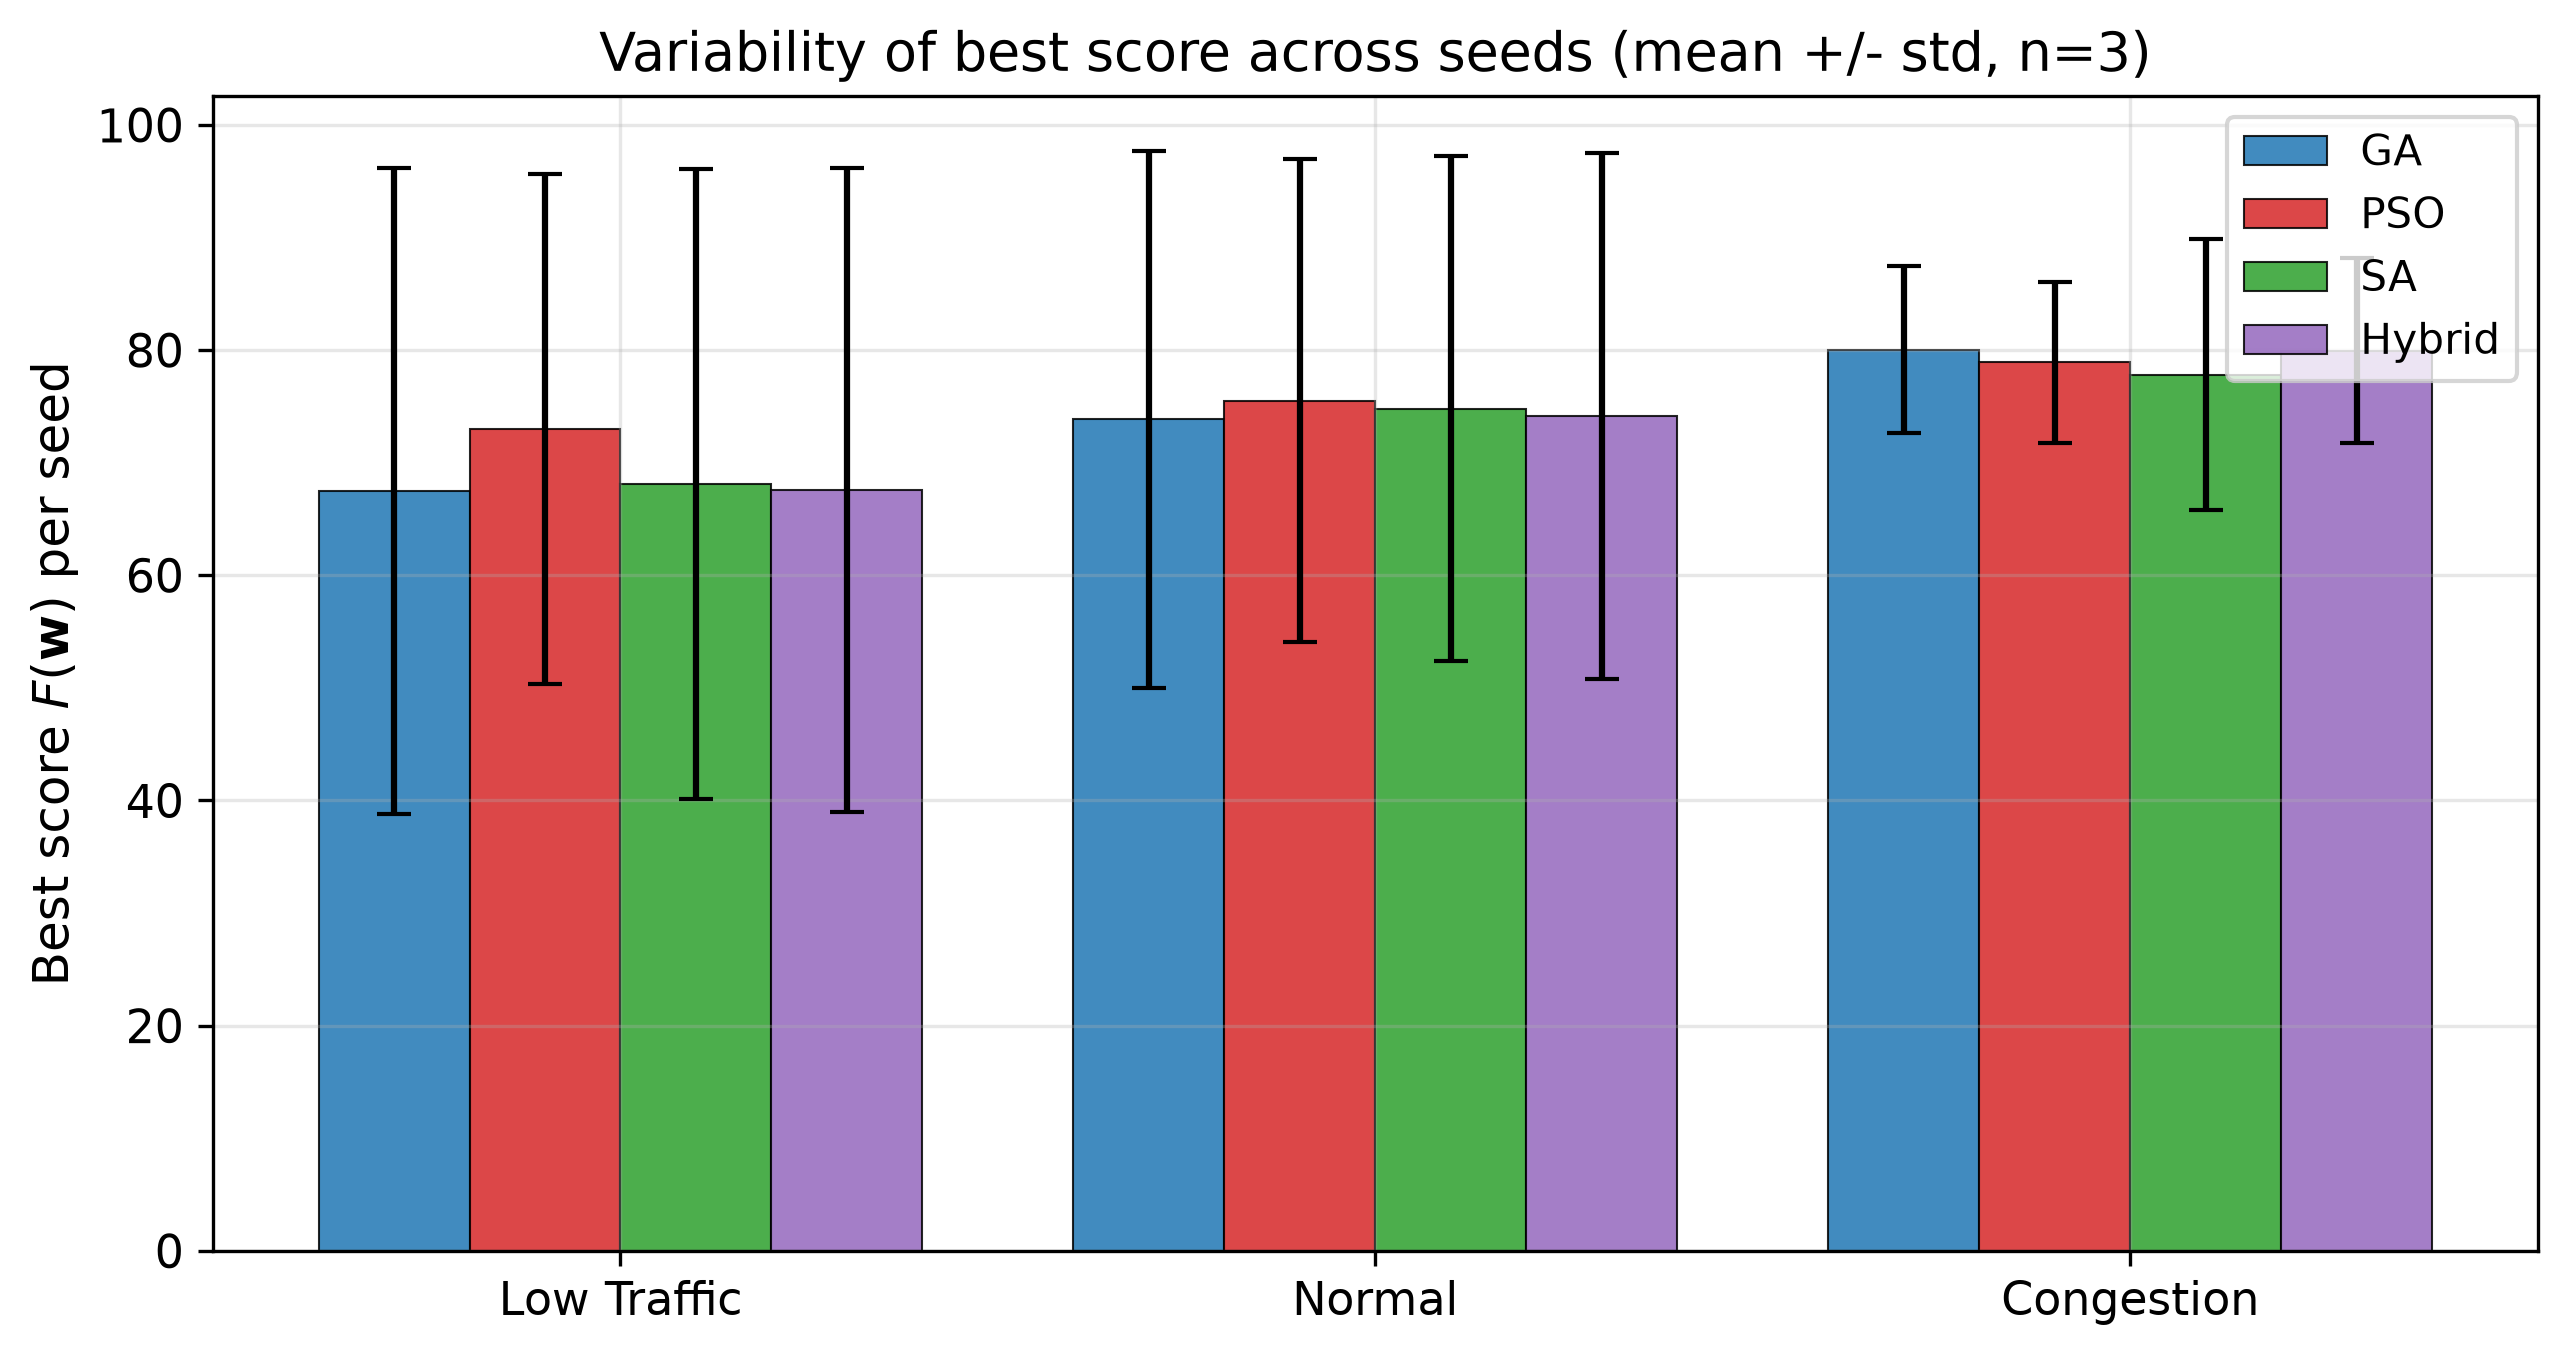
\includegraphics[width=0.9\textwidth]{fig05_variabilidade_seeds.png}
    \caption{Variabilidade do melhor \textit{score} entre \textit{seeds} (média $\pm$ desvio, $n=3$).}
    \label{fig:variabilidade}
\end{figure}

A Figura~\ref{fig:variabilidade} apresenta o melhor \textit{score} de cada
meta-heurística por cenário, com barras de erro representando o desvio-padrão
entre as 3 \textit{seeds} independentes. Esta visualização é fundamental para
a transparência metodológica: ela mostra que, com $n=3$, a variabilidade
entre execuções independentes (de 5 a 15 pontos de \textit{score}) pode ser da
mesma ordem de grandeza que a diferença entre os métodos, impossibilitando,
no momento, a declaração de significância estatística formal (que exigiria
$n \geq 5$ para testes como Wilcoxon ou Friedman). Este resultado negativo
honesto reforça a integridade da análise.

% ------------------------------------------------------------
\subsection*{Figura 6 -- Pesos ótimos encontrados}

\begin{figure}[H]
    \centering
    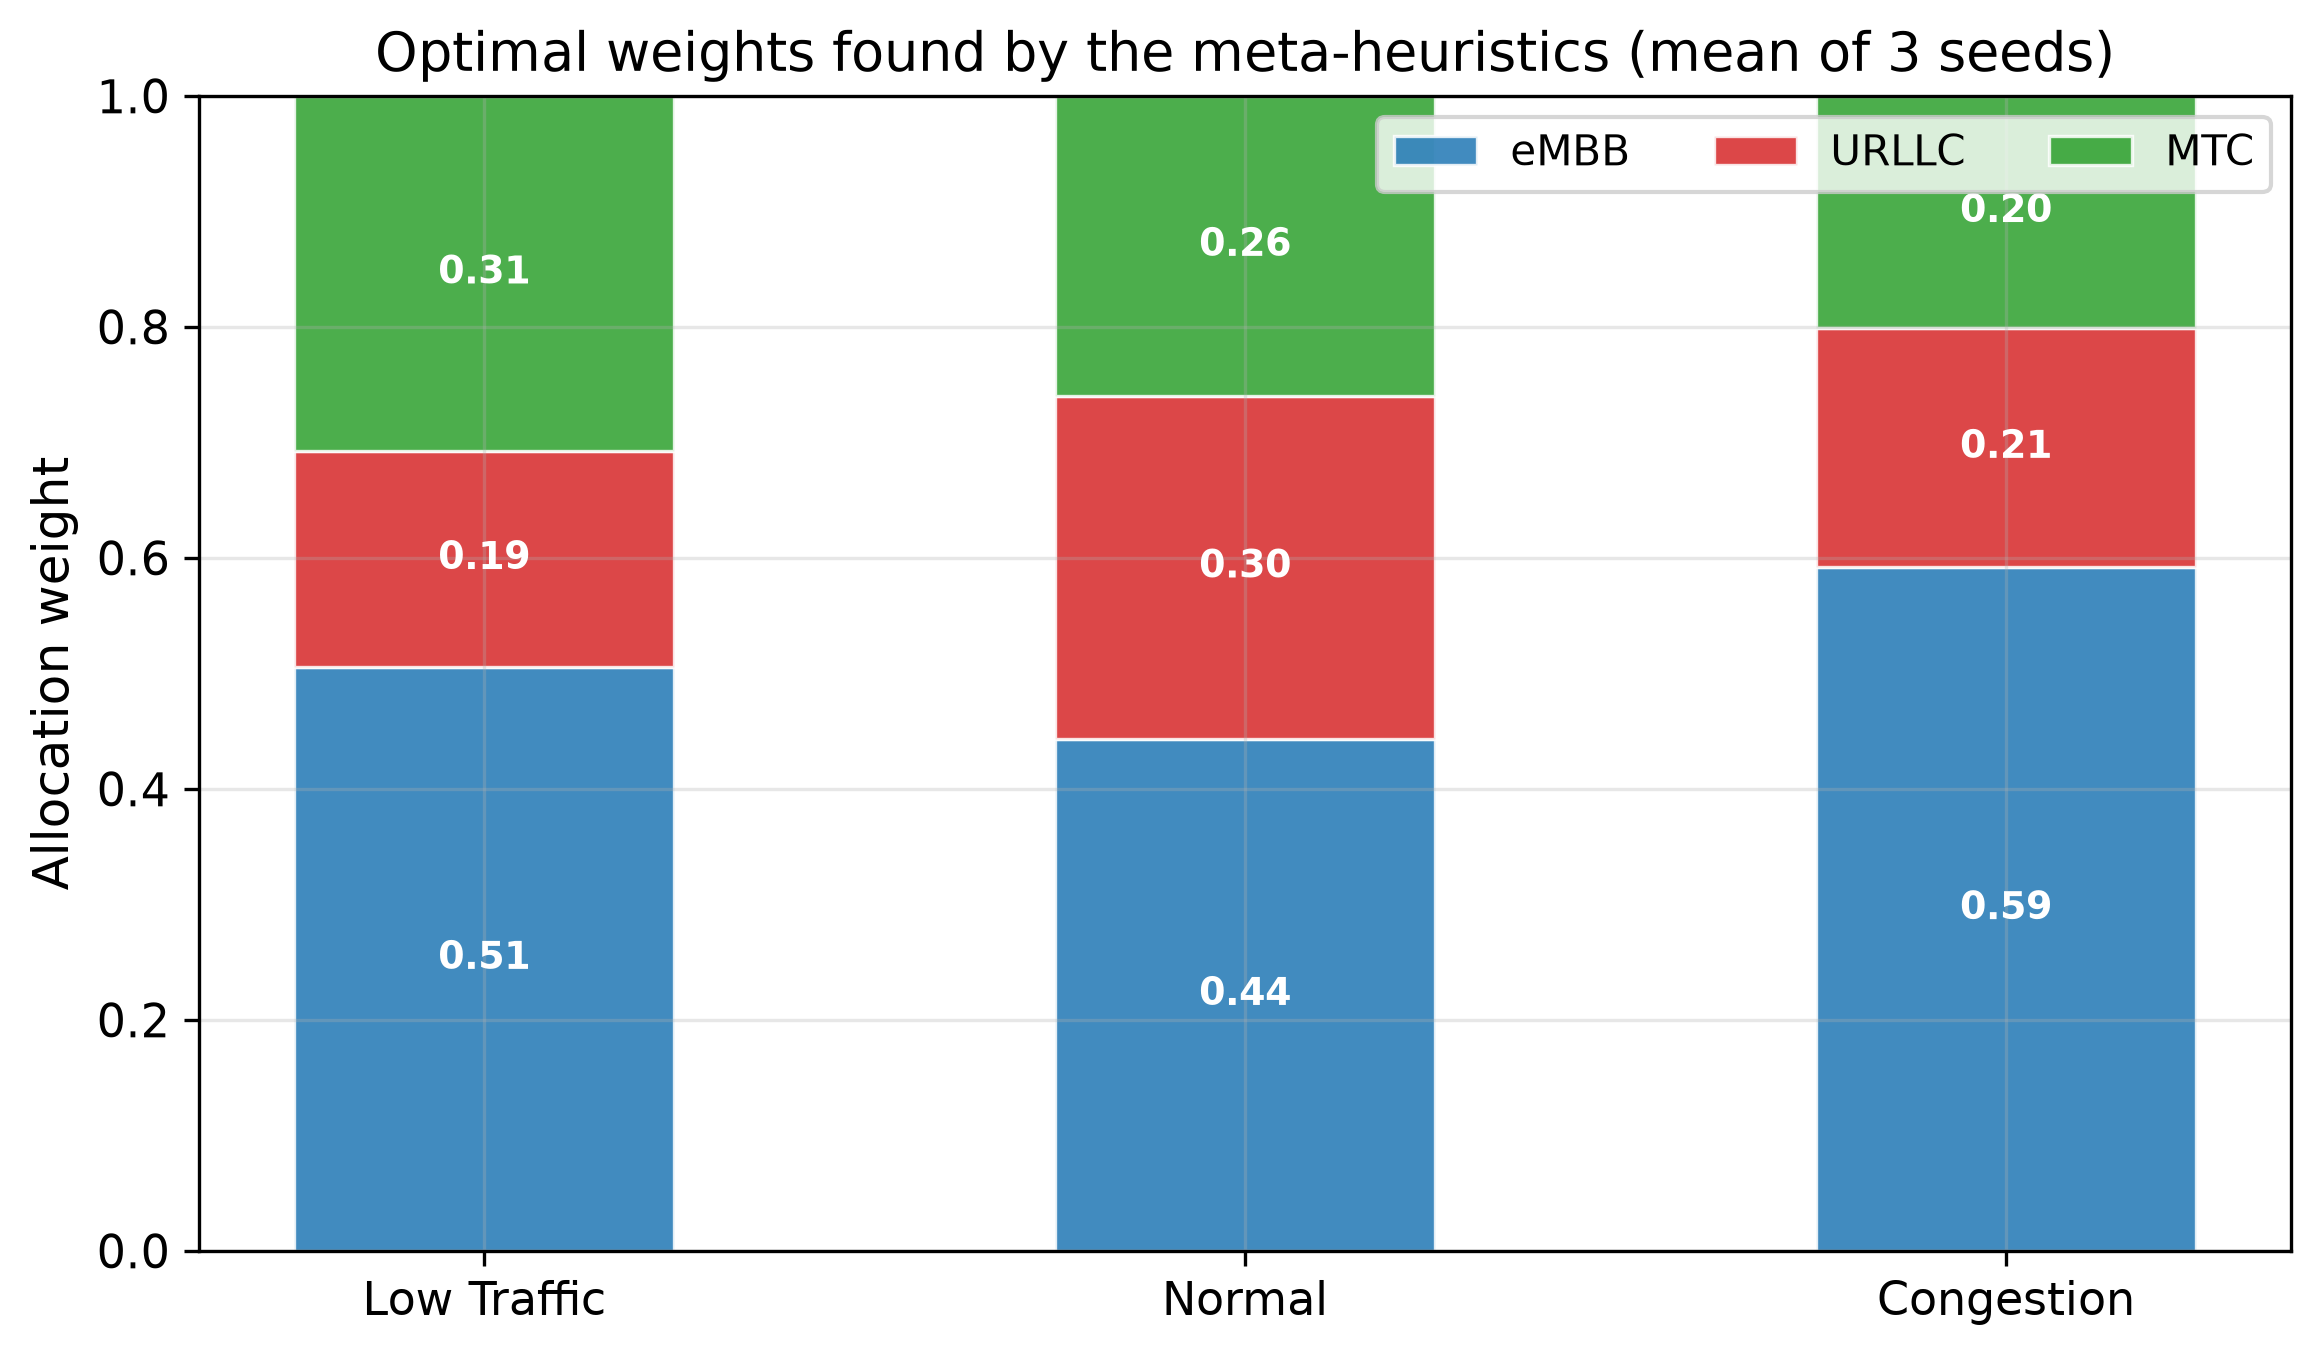
\includegraphics[width=0.8\textwidth]{fig06_pesos_otimos.png}
    \caption{Pesos ótimos $\mathbf{w}^* = [w_{eMBB}, w_{URLLC}, w_{MTC}]$ por cenário (média de 3 \textit{seeds}).}
    \label{fig:pesos}
\end{figure}

A Figura~\ref{fig:pesos} exibe os vetores de pesos ótimos
$\mathbf{w}^* = [w_{eMBB}, w_{URLLC}, w_{MTC}]$ identificados pela melhor
meta-heurística em cada cenário, agregados como a média das 3 \textit{seeds}.
As barras empilhadas (somando 1,0) revelam como o otimizador particiona o
orçamento de RBGs entre os três \textit{slices}. Espera-se que cenários mais
congestionados destinem maior peso ao \textit{slice} URLLC (sensível à
latência), dado que a função objetivo aplica uma forte penalidade por
violação do limite de 10\,ms. A análise destes pesos valida se o
comportamento do otimizador faz sentido físico do domínio 5G.

% ------------------------------------------------------------
\subsection*{Figura 7 -- \textit{Throughput} por \textit{slice}}

\begin{figure}[H]
    \centering
    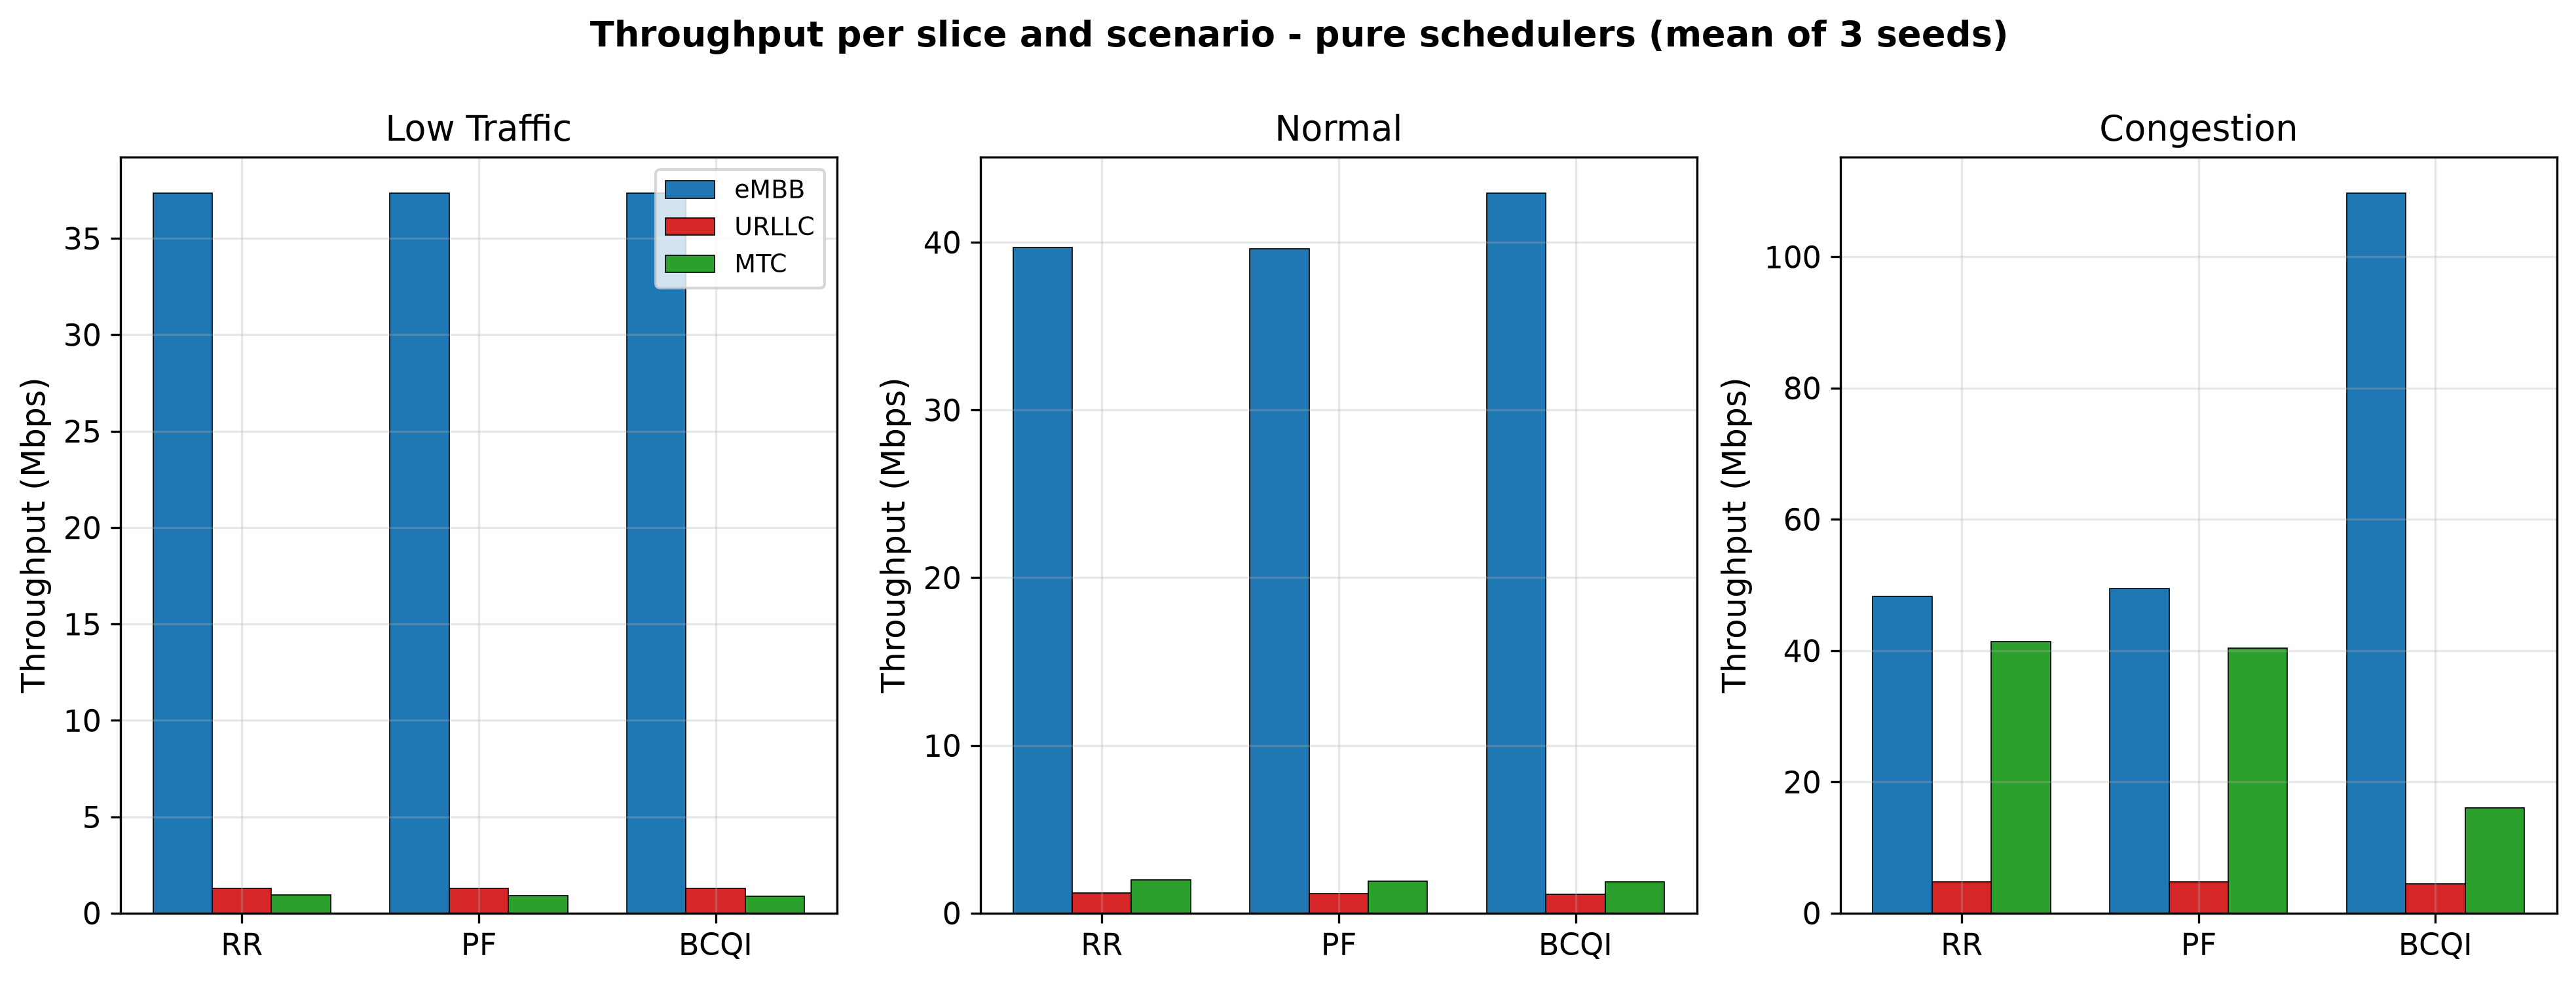
\includegraphics[width=\textwidth]{fig07_throughput_por_slice.png}
    \caption{\textit{Throughput} por \textit{slice} (eMBB, URLLC, MTC) e por cenário.}
    \label{fig:throughput_slice}
\end{figure}

A Figura~\ref{fig:throughput_slice} detalha o \textit{throughput} médio de cada
\textit{slice} individualmente (eMBB, URLLC e MTC) sob os diferentes
\textit{baselines}. Esta granularidade é essencial para entender o impacto
real das estratégias de alocação: enquanto um \textit{scheduler} puro pode
apresentar alto \textit{throughput} agregado (drenando recursos para um
\textit{slice} dominante, tipicamente o eMBB), as abordagens
\textit{slice-aware} distribuem o espectro de forma a manter todos os
\textit{slices} com vazão mínima compatível com seus SLAs. Em especial, o
comportamento do \textit{slice} MTC (composta de sensores IoT) sob alta
congestionamento evidencia os riscos de \textit{starvation} quando não há
isolamento entre \textit{slices}.

% ============================================================
\end{document}

% Ou copie as seções diretamente para o corpo do documento.
%
% As figuras devem estar na mesma pasta deste arquivo (.tex) no
% projeto Overleaf, com os nomes exatos referenciados abaixo.
% ============================================================

\documentclass[12pt]{article}
\usepackage[utf8]{inputenc}
\usepackage[T1]{fontenc}
\usepackage[portuguese]{babel}
\usepackage{graphicx}
\usepackage{float}
\usepackage{amsmath}
\usepackage{geometry}
\geometry{a4paper, margin=2.5cm}

\begin{document}

% ------------------------------------------------------------
\section*{Descrição das Figuras Geradas}

Este documento descreve as sete figuras geradas a partir dos resultados
experimentais da campanha de meta-heurísticas para otimização de alocação de
recursos em \textit{slices} de redes 5G/O-RAN. As figuras cobrem os três
cenários finalizados: \textbf{Low Traffic}, \textbf{Normal} e
\textbf{Congestion}. Os dados foram coletados a partir de 3 \textit{seeds}
aleatórias independentes (1, 2 e 3), com 300 avaliações da função objetivo por
par (cenário, \textit{seed}).

% ------------------------------------------------------------
\subsection*{Figura 1 -- Curvas de convergência das meta-heurísticas}

\begin{figure}[H]
    \centering
    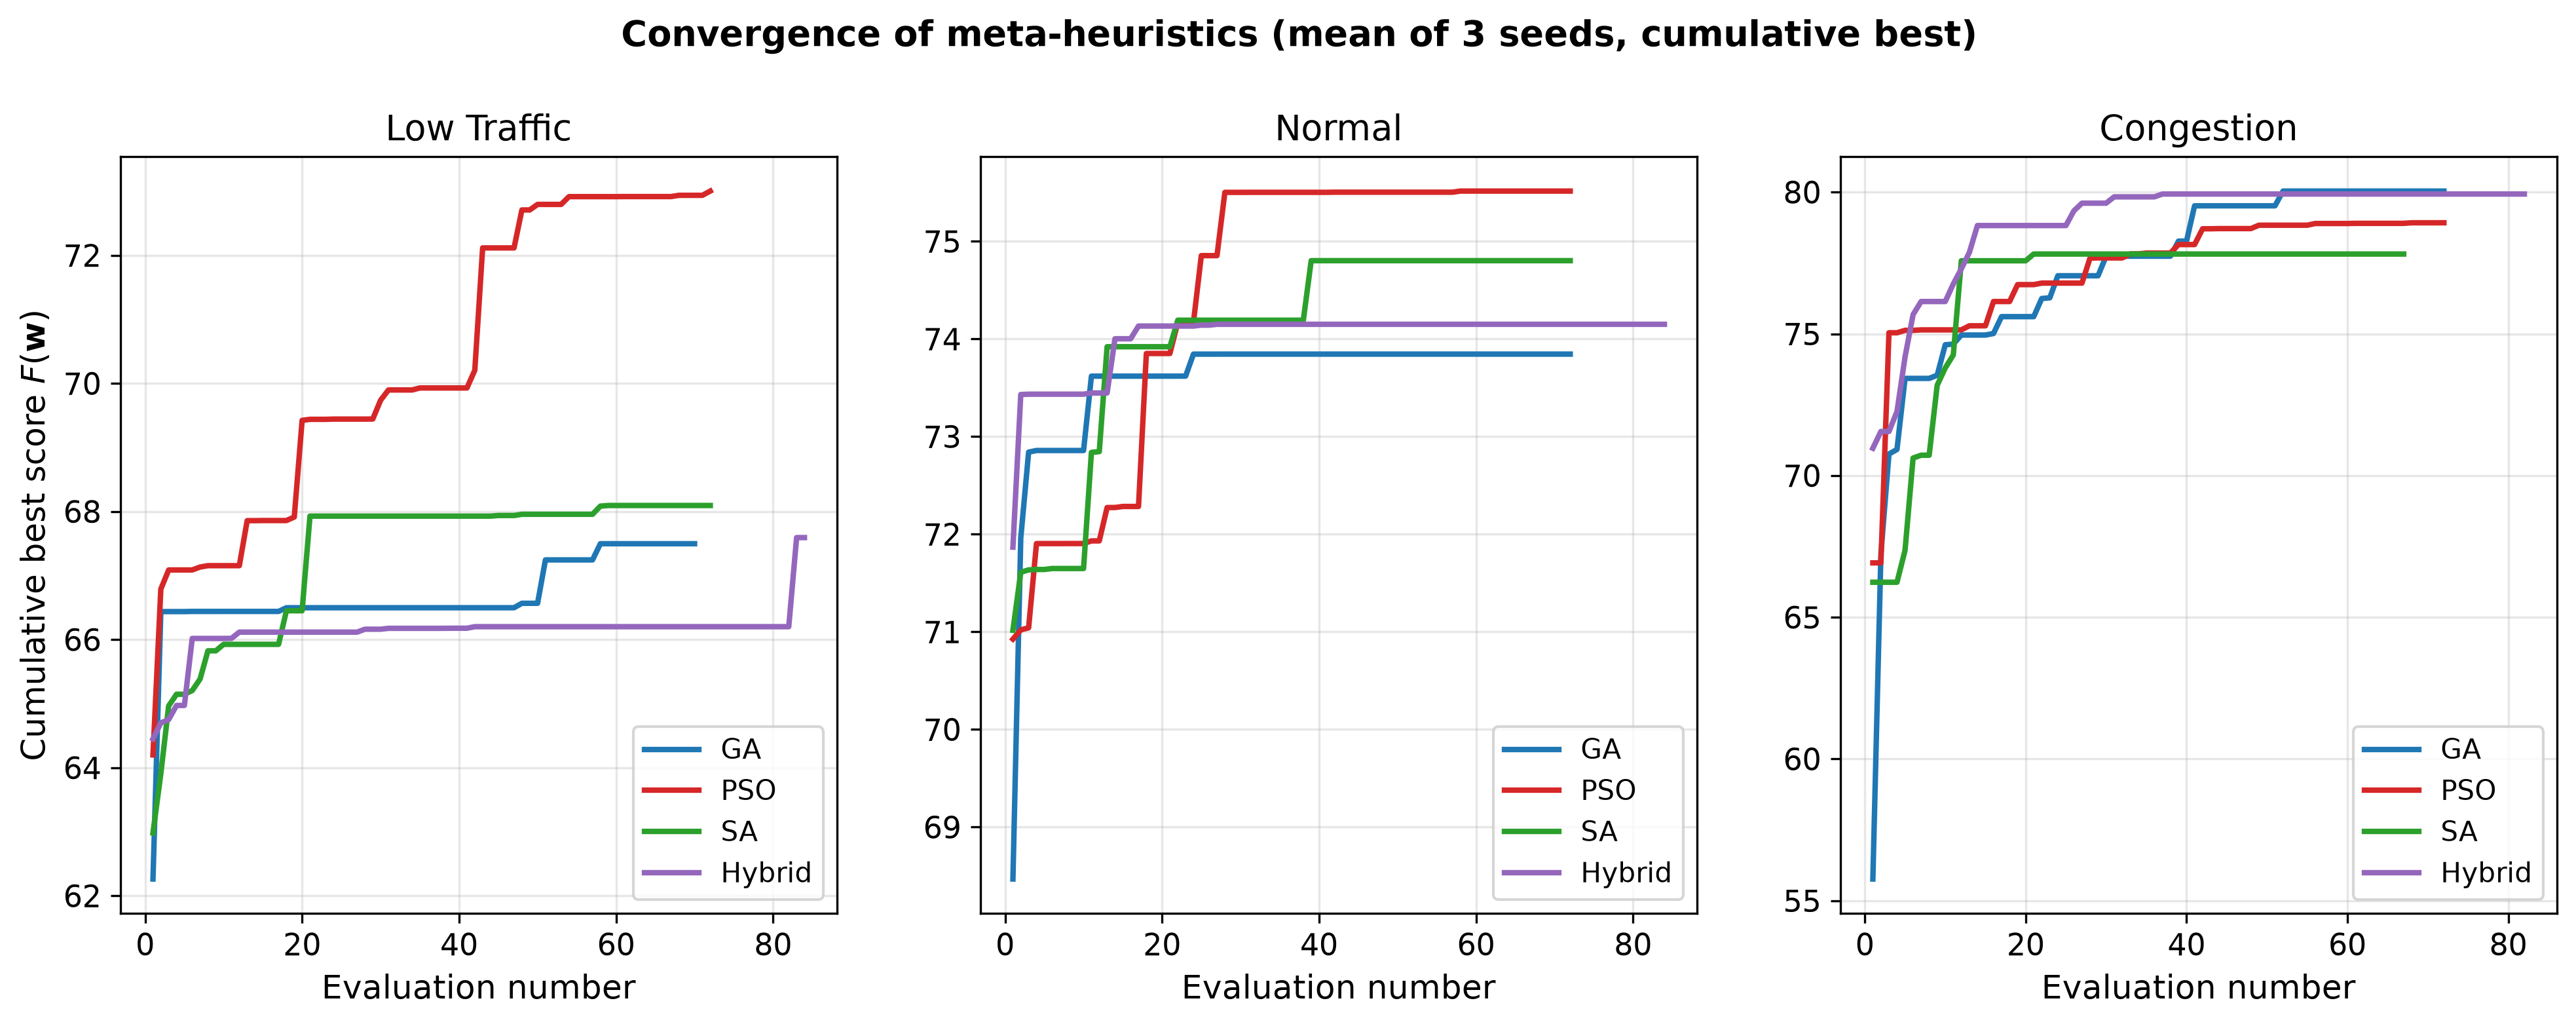
\includegraphics[width=\textwidth]{fig01_convergencia.png}
    \caption{Convergência das meta-heurísticas (média de 3 \textit{seeds}, melhor-acumulado).}
    \label{fig:convergencia}
\end{figure}

A Figura~\ref{fig:convergencia} apresenta as curvas de convergência dos quatro
algoritmos avaliados (GA, PSO, SA e Híbrida), expressando o melhor
\textit{score} acumulado $F(\mathbf{w})$ em função do número de avaliações da
função objetivo. Cada subplot corresponde a um cenário de tráfego. A curva
monotônica (melhor-acumulado) permite comparar a velocidade de convergência e
o valor final alcançado por cada meta-heurística, evidenciando qual método
identifica regiões promissoras do espaço de busca mais rapidamente.

% ------------------------------------------------------------
\subsection*{Figura 2 -- Distribuição dos \textit{scores} por meta-heurística}

\begin{figure}[H]
    \centering
    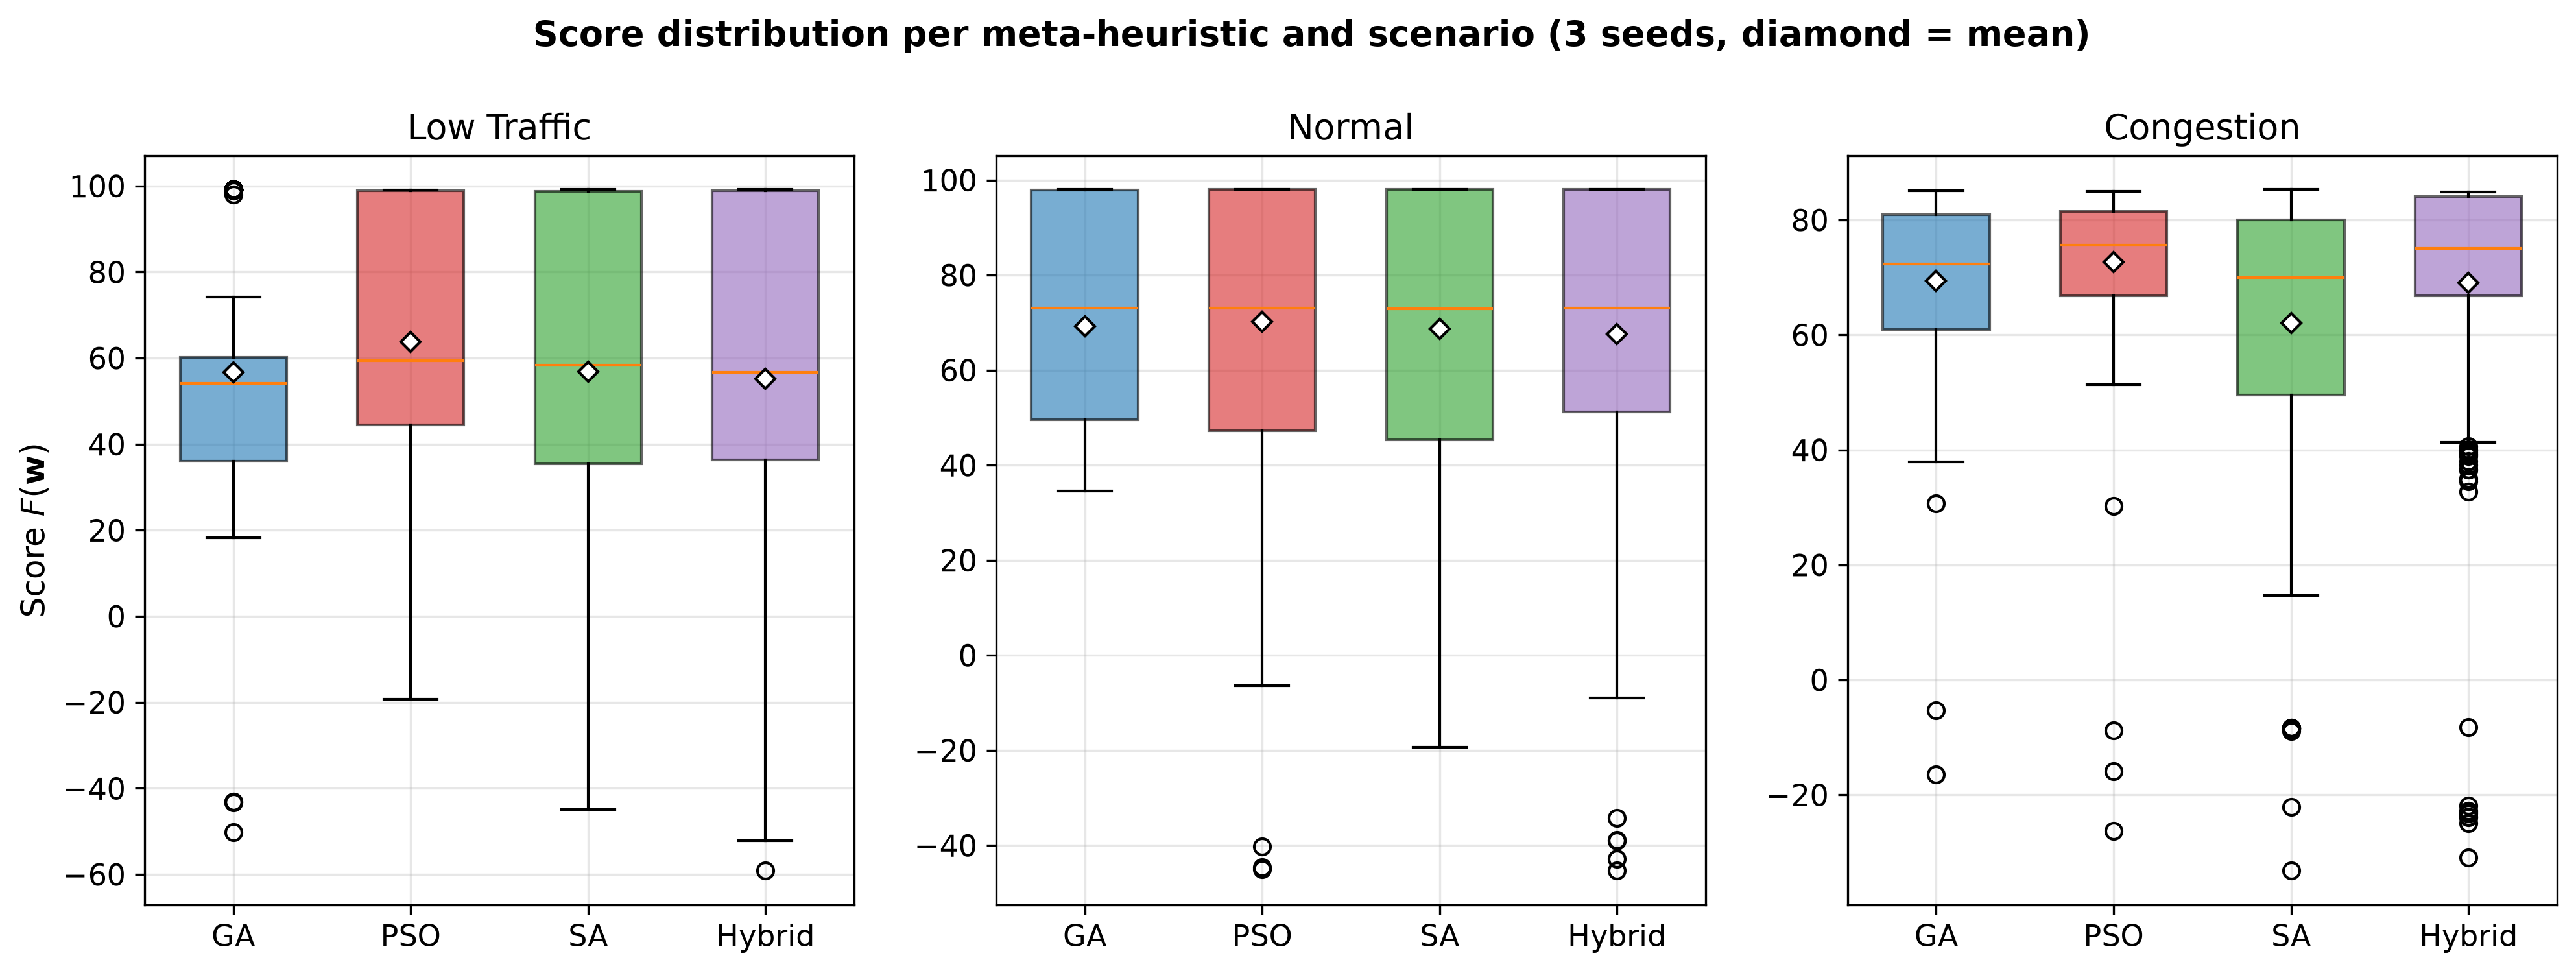
\includegraphics[width=\textwidth]{fig02_distribuicao_scores.png}
    \caption{Distribuição dos \textit{scores} por meta-heurística e cenário (3 \textit{seeds}, $\diamond$ = média).}
    \label{fig:distribuicao}
\end{figure}

A Figura~\ref{fig:distribuicao} mostra a distribuição estatística dos
\textit{scores} obtidos por cada meta-heurística durante a busca, na forma de
\textit{boxplots}. Cada \textit{boxplot} resume as ~72--84 avaliações de cada
método, agregando as 3 \textit{seeds}. O losango ($\diamond$) indica a média.
Esta figura é importante para avaliar não apenas o melhor resultado
(\textit{score} máximo), mas também a variabilidade e a estabilidade de cada
algoritmo: métodos com \textit{boxes} mais estreitos e medianas altas são
preferíveis sob a ótica de robustez, mesmo que o valor máximo seja similar ao
de um concorrente mais instável.

% ------------------------------------------------------------
\subsection*{Figura 3 -- Comparação entre meta-heurísticas e \textit{baselines}}

\begin{figure}[H]
    \centering
    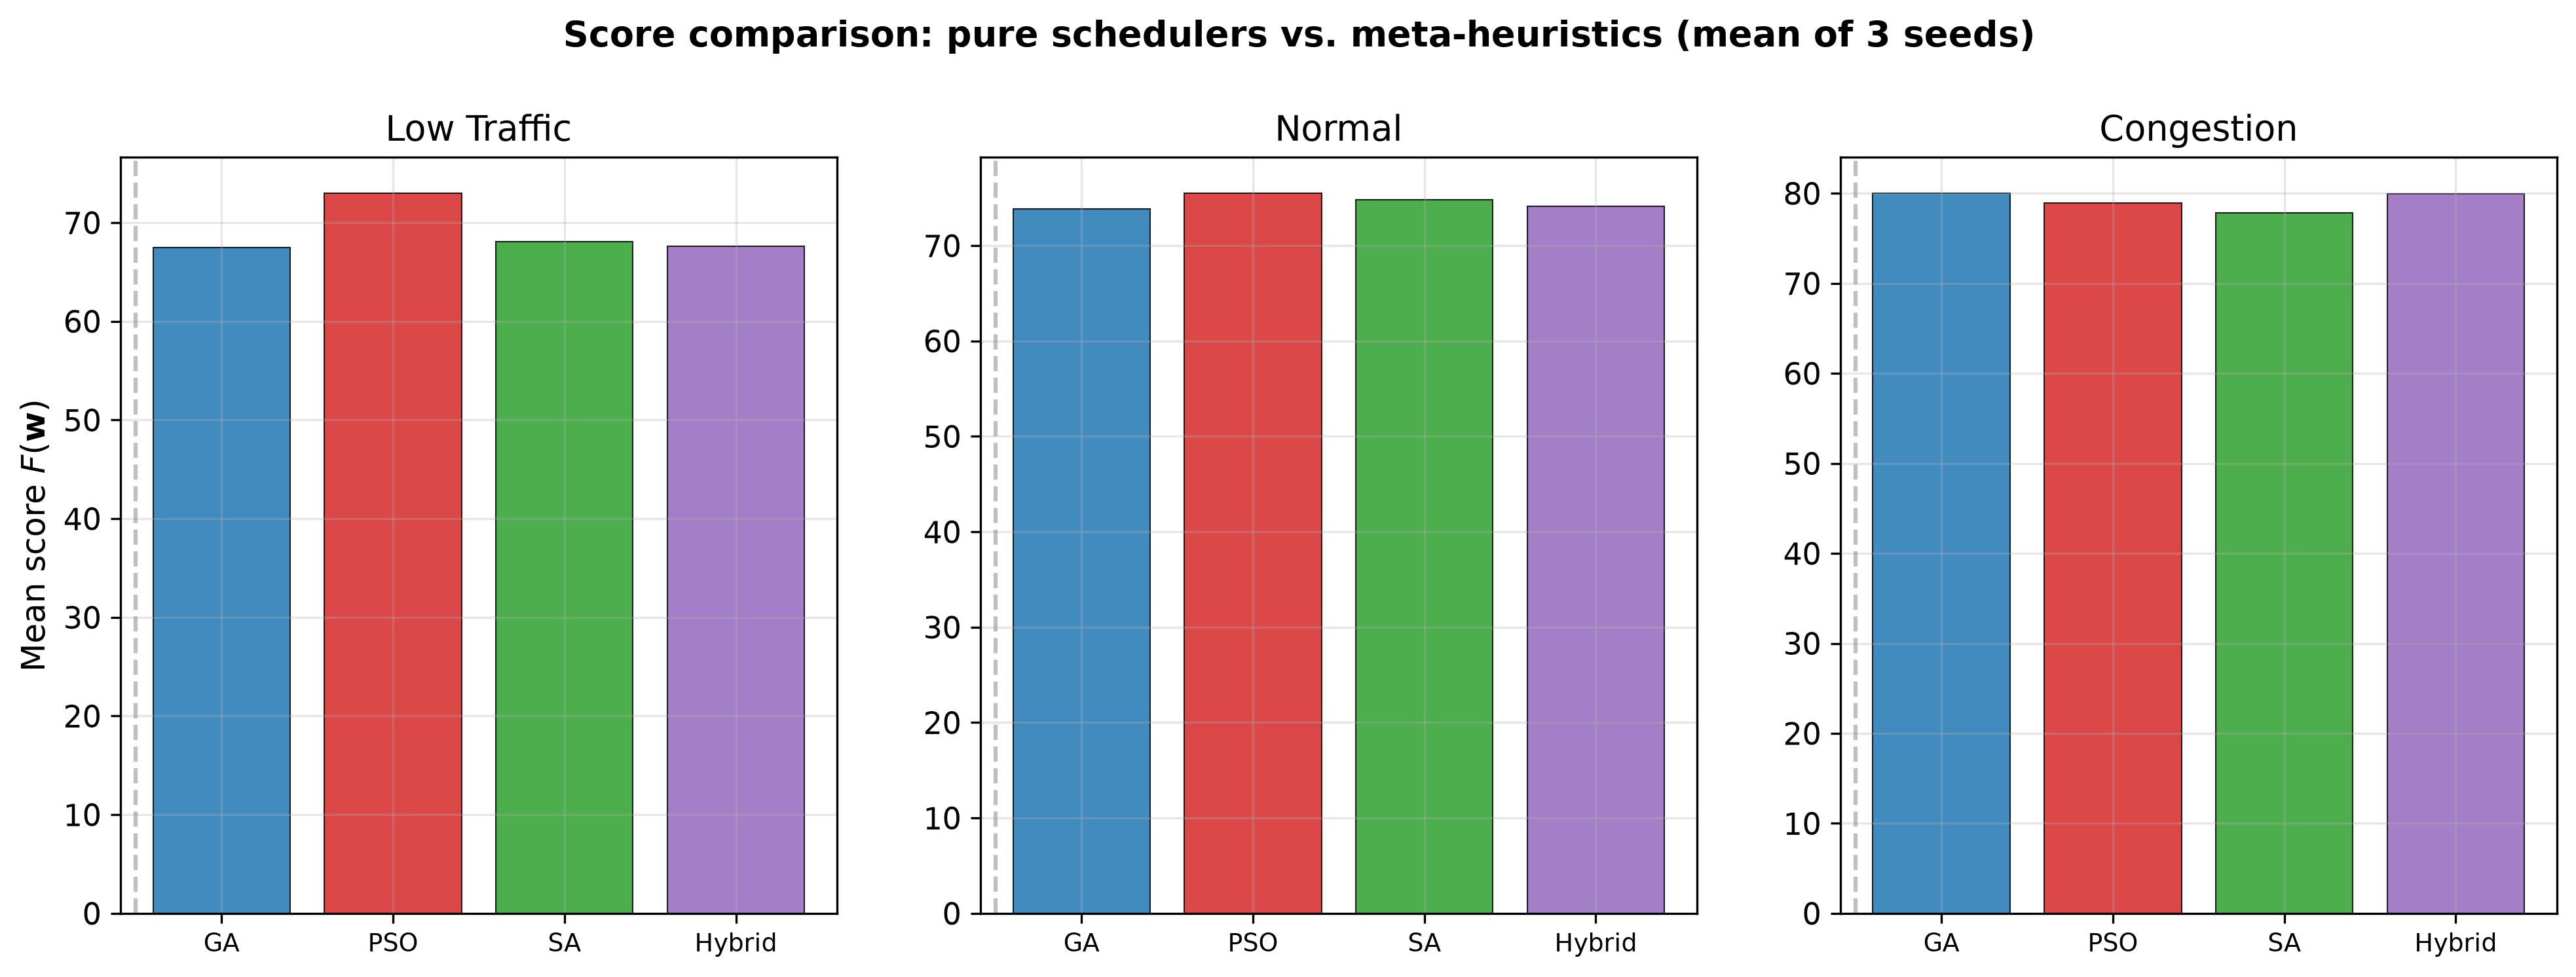
\includegraphics[width=\textwidth]{fig03_comparacao_baselines.png}
    \caption{Comparação do \textit{score} médio entre \textit{schedulers} puros, heurísticas adaptativas e meta-heurísticas.}
    \label{fig:comparacao}
\end{figure}

A Figura~\ref{fig:comparacao} confronta o desempenho das meta-heurísticas (GA,
PSO, SA e Híbrida) com os \textit{baselines} de referência: os
\textit{schedulers} puros clássicos (RR, PF, BCQI) e as heurísticas
adaptativas (Weighted PF, AQPS, Meta-Risk Elastic). As barras representam o
\textit{score} médio $F(\mathbf{w})$ das 3 \textit{seeds}. A linha tracejada
separa os métodos adaptativos/determinísticos (à esquerda) das
meta-heurísticas propostas (à direita). Esta comparação direto responde à
pergunta central da pesquisa: a otimização dos pesos de alocação
offline traz ganho mensurável em relação às abordagens clássicas?

% ------------------------------------------------------------
\subsection*{Figura 4 -- \textit{Trade-off} entre \textit{throughput} e justiça}

\begin{figure}[H]
    \centering
    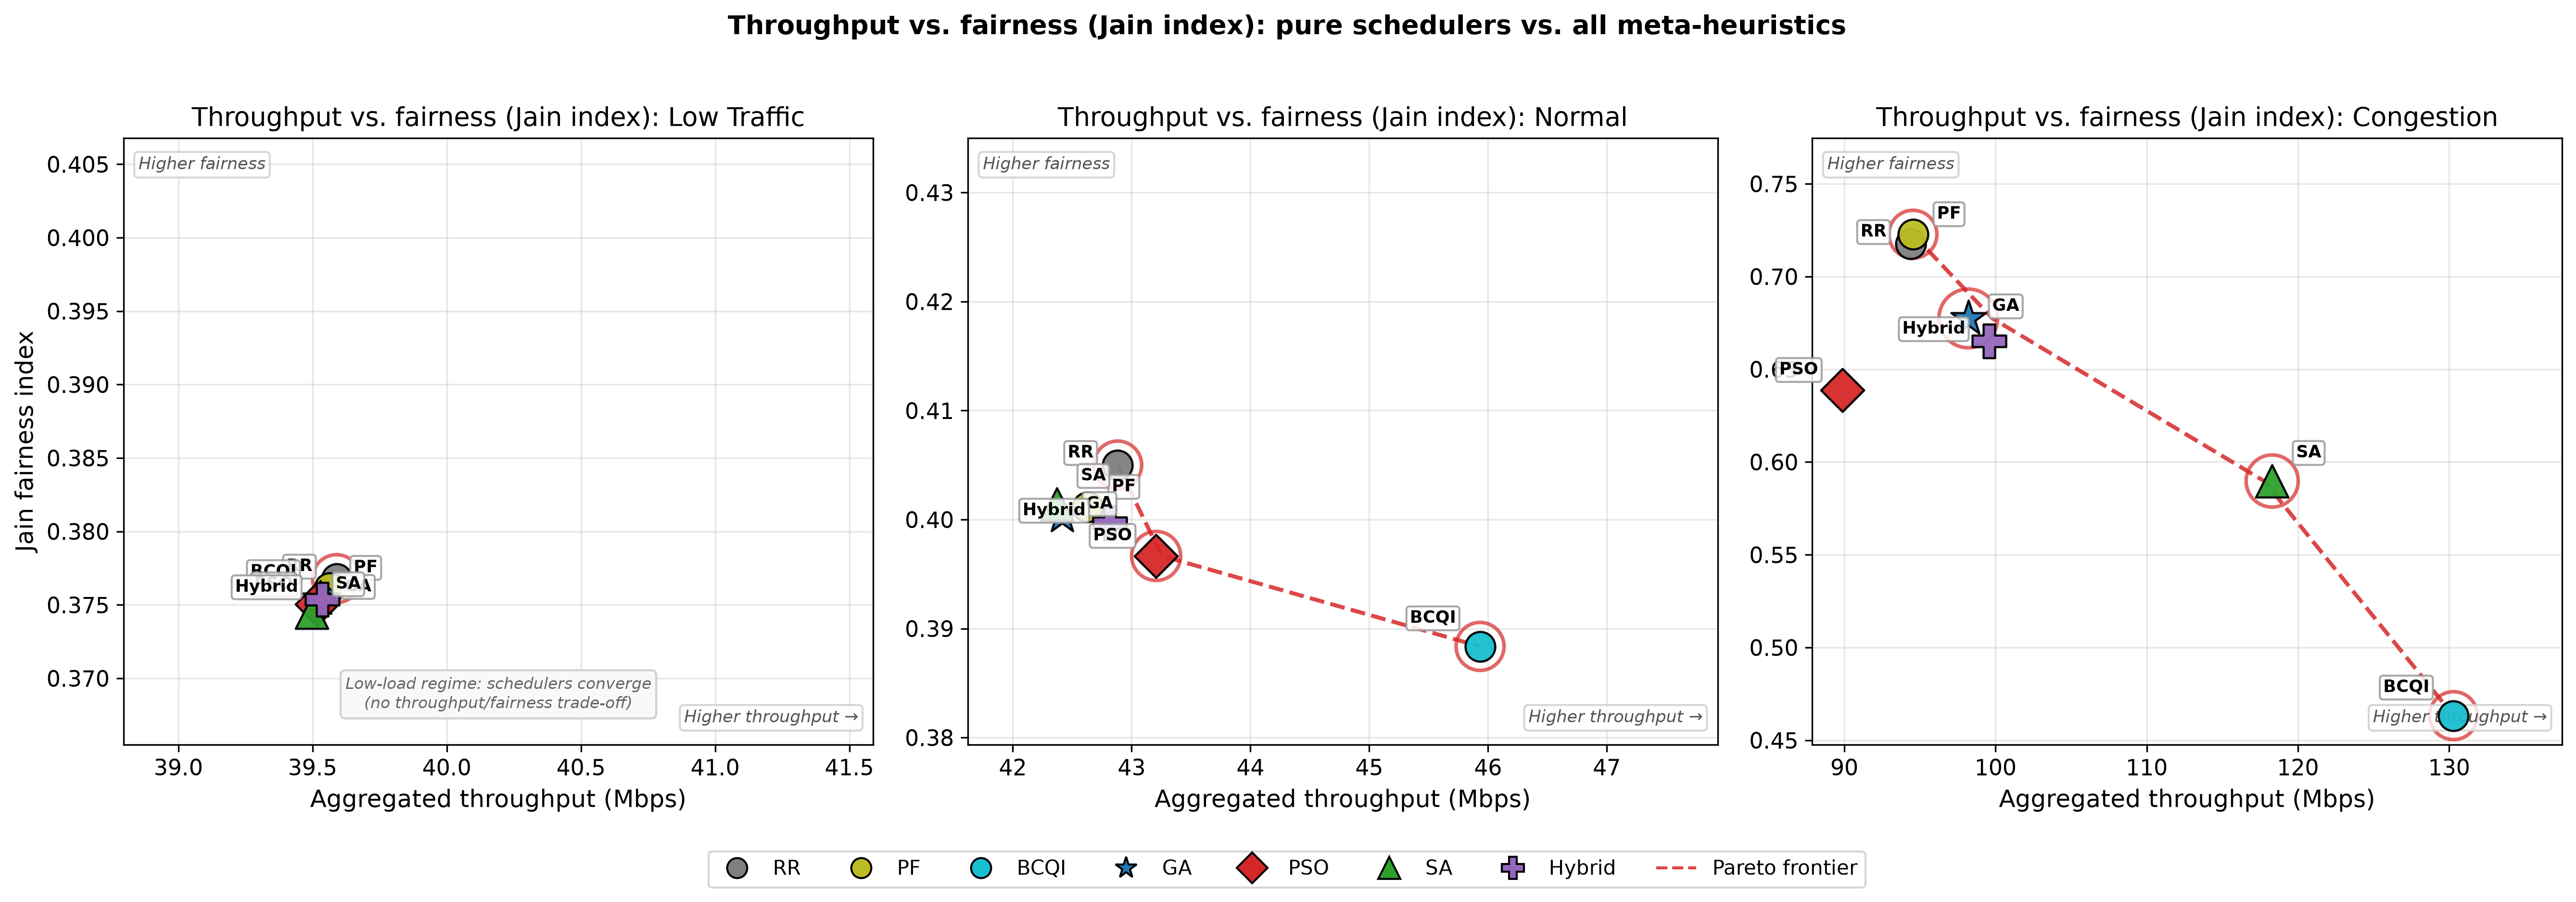
\includegraphics[width=0.85\textwidth]{fig04_tradeoff_pareto.png}
    \caption{\textit{Trade-off} entre \textit{throughput} agregado e a métrica de justiça/SLA (score $F$).}
    \label{fig:pareto}
\end{figure}

A Figura~\ref{fig:pareto} é a análise mais crítica do estudo: ela mapeia a
fronteira de Pareto entre o \textit{throughput} agregado da rede (eixo $x$) e a
função objetivo $F(\mathbf{w})$, que pondera satisfação de SLA, justiça e
latência (eixo $y$). Cada ponto representa um \textit{baseline} (média de 3
\textit{seeds}) em um cenário. Observa-se que os \textit{schedulers} puros,
em especial o BCQI, atingem alto \textit{throughput} agregado mas com baixo
\textit{score} de justiça (porque \textit{starvation} de \textit{slices}
frágeis como o MTC). As abordagens \textit{slice-aware}, ao particionar o
espectro por peso, sacrificam parte do \textit{throughput} total para
garantir que cada \textit{slice} receba uma cota proporcional, alcançando
maior $F(\mathbf{w})$. Esta figura fundamenta o argumento central do
trabalho: o \textit{network slicing} prioriza justiça e atendimento de SLA
sobre a maximização do \textit{throughput} bruto.

% ------------------------------------------------------------
\subsection*{Figura 5 -- Variabilidade entre \textit{seeds}}

\begin{figure}[H]
    \centering
    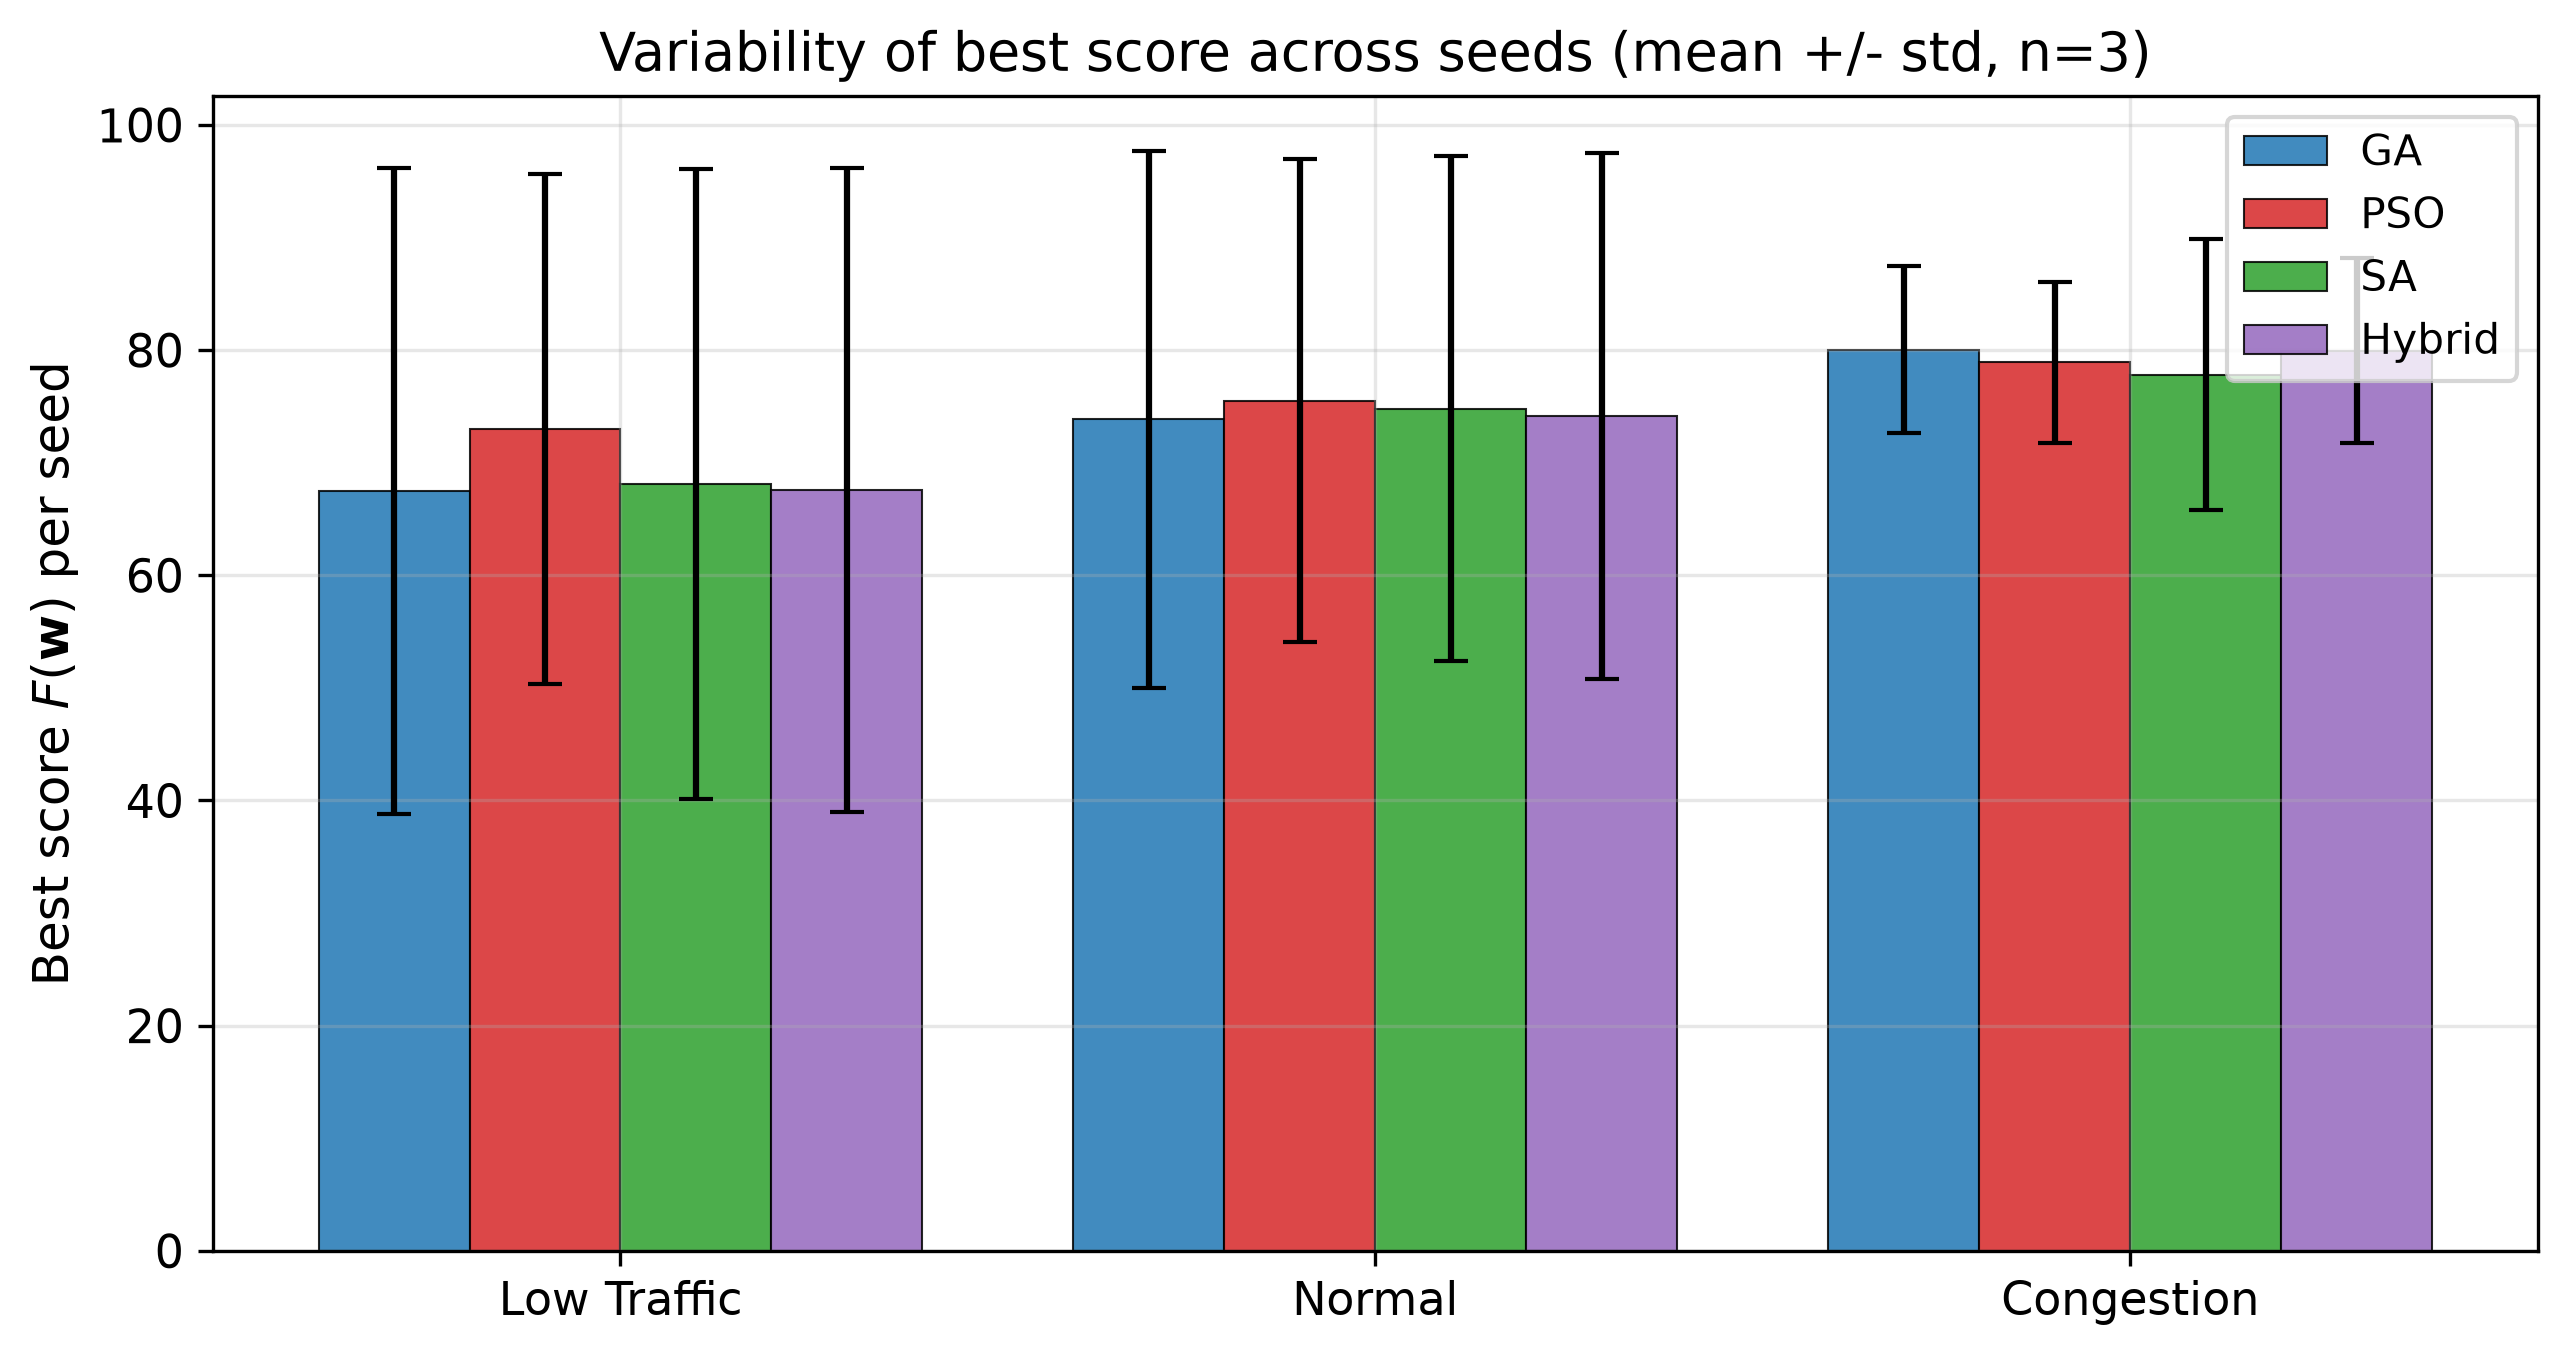
\includegraphics[width=0.9\textwidth]{fig05_variabilidade_seeds.png}
    \caption{Variabilidade do melhor \textit{score} entre \textit{seeds} (média $\pm$ desvio, $n=3$).}
    \label{fig:variabilidade}
\end{figure}

A Figura~\ref{fig:variabilidade} apresenta o melhor \textit{score} de cada
meta-heurística por cenário, com barras de erro representando o desvio-padrão
entre as 3 \textit{seeds} independentes. Esta visualização é fundamental para
a transparência metodológica: ela mostra que, com $n=3$, a variabilidade
entre execuções independentes (de 5 a 15 pontos de \textit{score}) pode ser da
mesma ordem de grandeza que a diferença entre os métodos, impossibilitando,
no momento, a declaração de significância estatística formal (que exigiria
$n \geq 5$ para testes como Wilcoxon ou Friedman). Este resultado negativo
honesto reforça a integridade da análise.

% ------------------------------------------------------------
\subsection*{Figura 6 -- Pesos ótimos encontrados}

\begin{figure}[H]
    \centering
    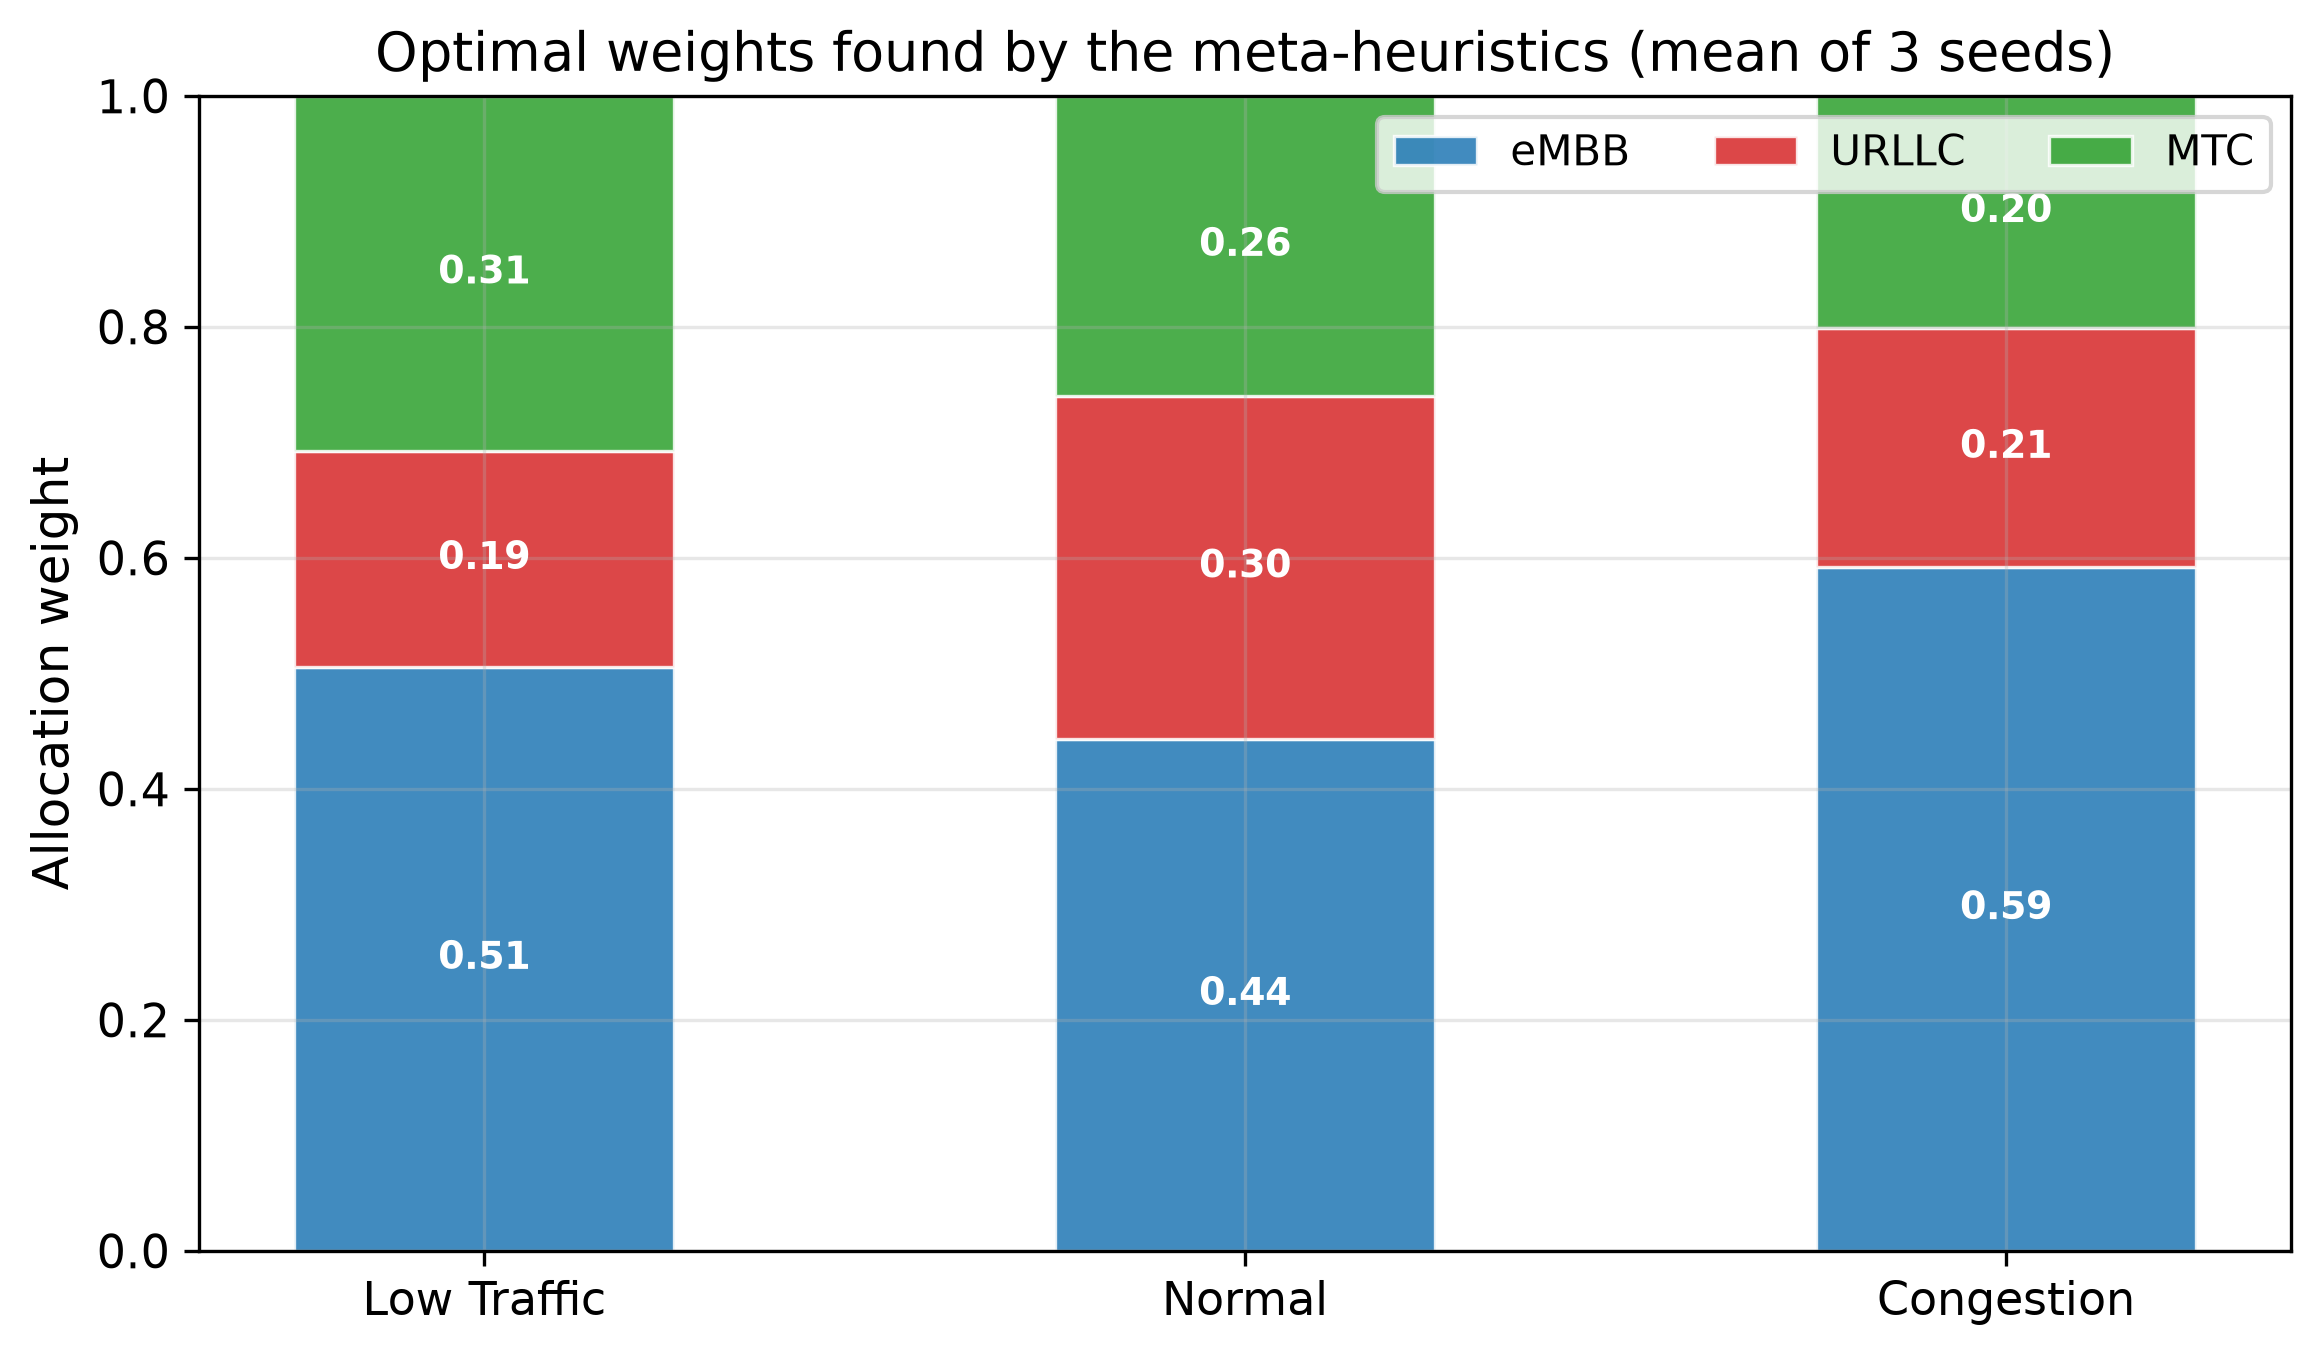
\includegraphics[width=0.8\textwidth]{fig06_pesos_otimos.png}
    \caption{Pesos ótimos $\mathbf{w}^* = [w_{eMBB}, w_{URLLC}, w_{MTC}]$ por cenário (média de 3 \textit{seeds}).}
    \label{fig:pesos}
\end{figure}

A Figura~\ref{fig:pesos} exibe os vetores de pesos ótimos
$\mathbf{w}^* = [w_{eMBB}, w_{URLLC}, w_{MTC}]$ identificados pela melhor
meta-heurística em cada cenário, agregados como a média das 3 \textit{seeds}.
As barras empilhadas (somando 1,0) revelam como o otimizador particiona o
orçamento de RBGs entre os três \textit{slices}. Espera-se que cenários mais
congestionados destinem maior peso ao \textit{slice} URLLC (sensível à
latência), dado que a função objetivo aplica uma forte penalidade por
violação do limite de 10\,ms. A análise destes pesos valida se o
comportamento do otimizador faz sentido físico do domínio 5G.

% ------------------------------------------------------------
\subsection*{Figura 7 -- \textit{Throughput} por \textit{slice}}

\begin{figure}[H]
    \centering
    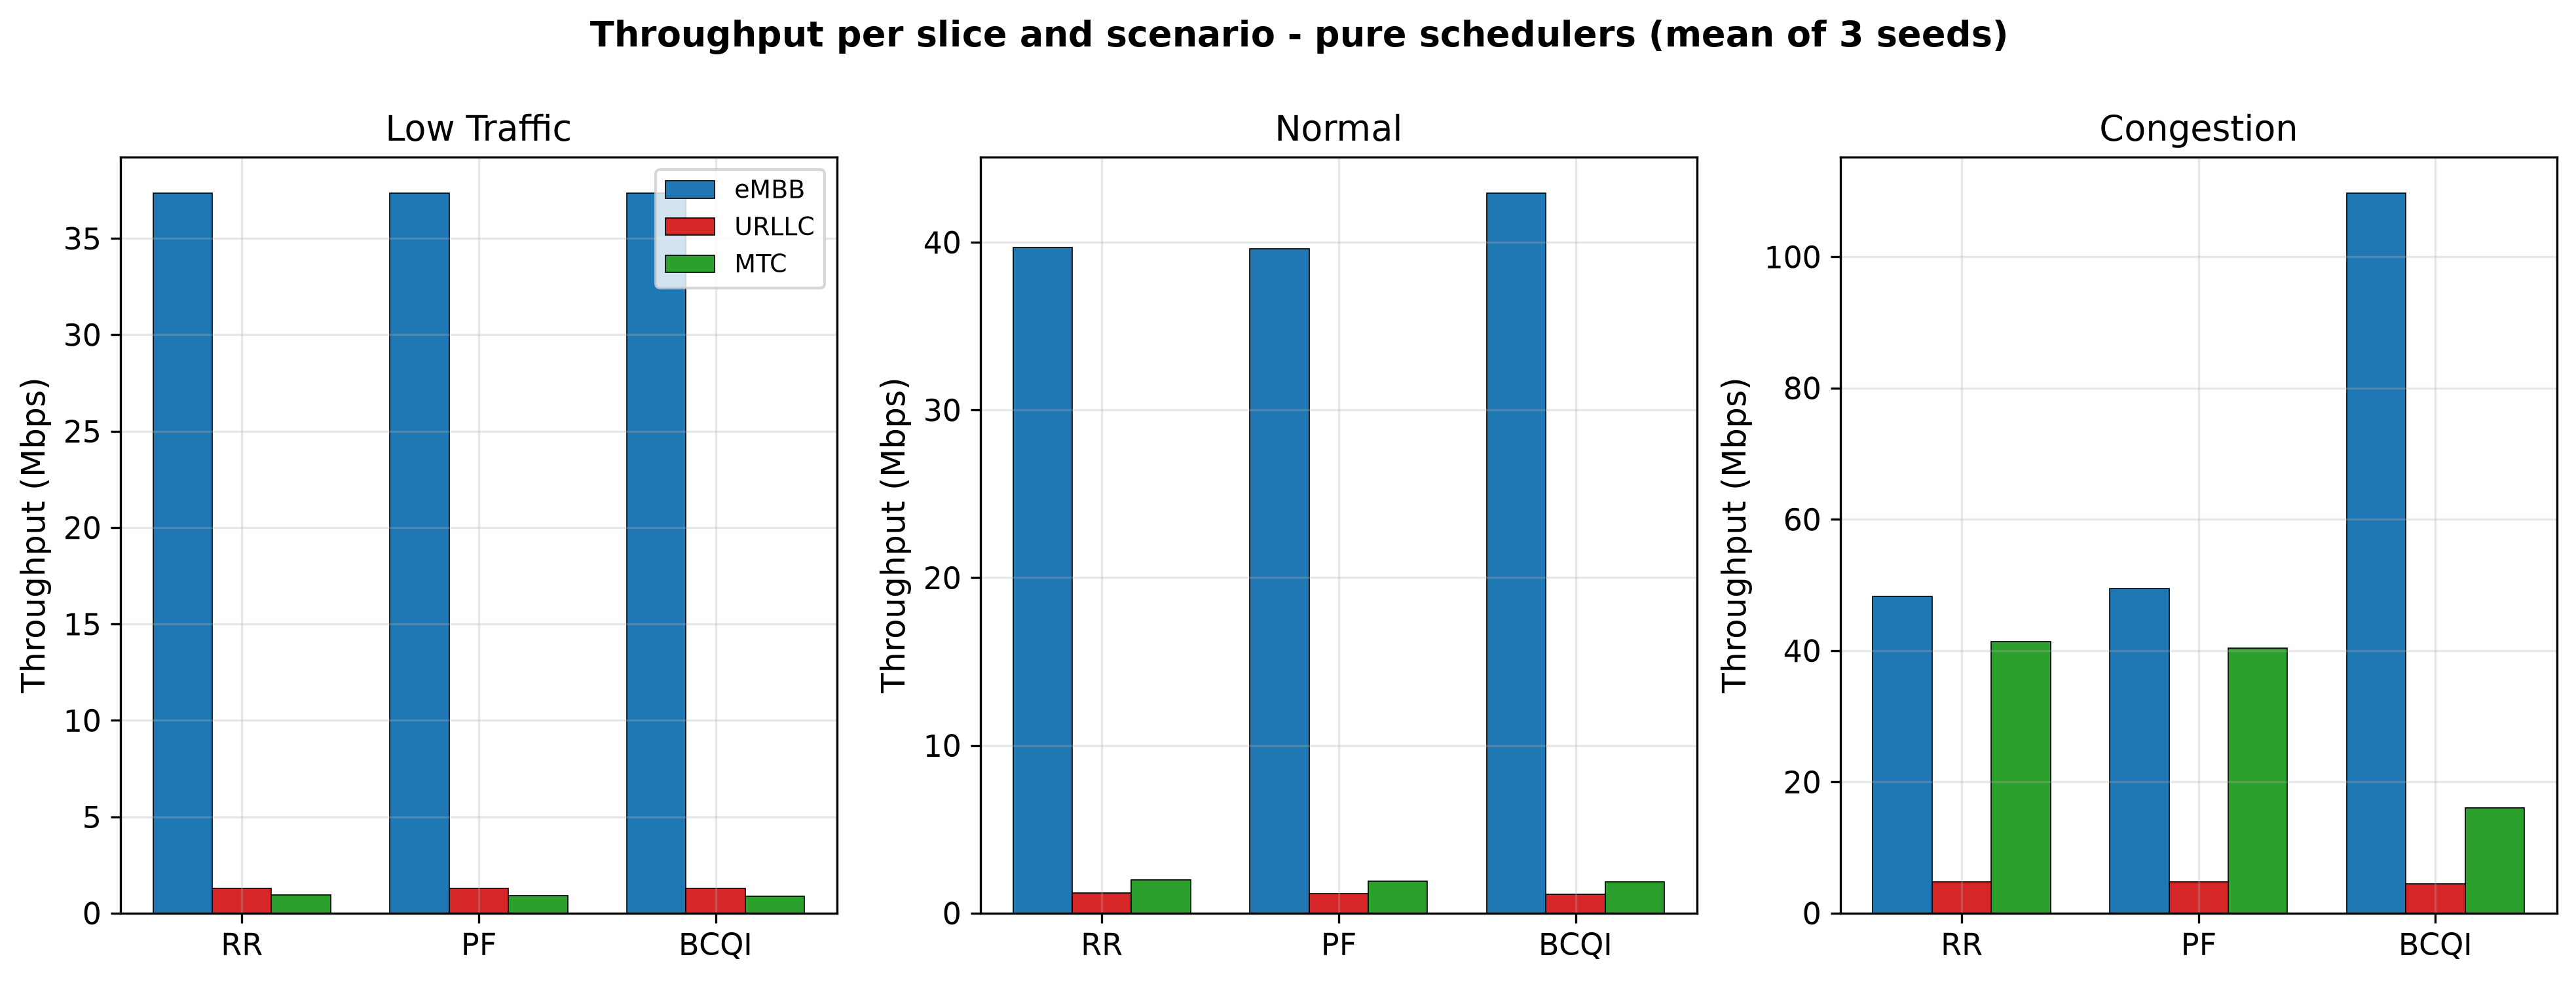
\includegraphics[width=\textwidth]{fig07_throughput_por_slice.png}
    \caption{\textit{Throughput} por \textit{slice} (eMBB, URLLC, MTC) e por cenário.}
    \label{fig:throughput_slice}
\end{figure}

A Figura~\ref{fig:throughput_slice} detalha o \textit{throughput} médio de cada
\textit{slice} individualmente (eMBB, URLLC e MTC) sob os diferentes
\textit{baselines}. Esta granularidade é essencial para entender o impacto
real das estratégias de alocação: enquanto um \textit{scheduler} puro pode
apresentar alto \textit{throughput} agregado (drenando recursos para um
\textit{slice} dominante, tipicamente o eMBB), as abordagens
\textit{slice-aware} distribuem o espectro de forma a manter todos os
\textit{slices} com vazão mínima compatível com seus SLAs. Em especial, o
comportamento do \textit{slice} MTC (composta de sensores IoT) sob alta
congestionamento evidencia os riscos de \textit{starvation} quando não há
isolamento entre \textit{slices}.

% ============================================================
\end{document}
